\documentclass[12pt]{report}
\usepackage[hidelinks]{hyperref}
\usepackage[T1]{fontenc}
\usepackage[utf8]{inputenc}
\usepackage[turkish,english,shorthands=:!]{babel}
\usepackage{apacite}
\usepackage[a4paper,width=155mm,top=25mm,bottom=25mm]{geometry}
\usepackage{epigraph}
\usepackage{graphicx}
%\graphicspath{ {graphics/} }
\usepackage{float}
\usepackage{caption}
\usepackage{subcaption}
\usepackage{wrapfig}
\usepackage[usenames,dvipsnames]{color}
\usepackage[titletoc]{appendix}
\usepackage[colorinlistoftodos]{todonotes}

%\usepackage{chngcntr}
%\counterwithout{figure}{chapter}

%\usepackage{setspace}
%\doublespacing

\setlength{\epigraphwidth}{.6\textwidth}
\setlength{\epigraphrule}{0pt}

\hypersetup{
    pdftitle			= {Thesis Draft},
    pdfauthor			= {Mustafa ilhan},
    pdfsubject			= {Trash, Art},
    pdfkeywords			= {mfa thesis, trash, art},
    colorlinks			= false,
    pdfborder			= {0 0 0},
    pdfpagemode			= UseOutlines
}

\providecommand{\quotes}[1]{``#1''}
\providecommand{\singlequotes}[1]{`#1'}
\providecommand{\comment}[1]{\textcolor{cyan}{#1}}
\providecommand{\paraphrase}[1]{\textcolor{magenta}{\quotes{#1}}}
\renewcommand*\bibname{Bibliography}


%****************************************
% Title Ideas for Thesis 
% - Trash as an Artistic Medium
% - Notebooks from Trash: Trash in the Context of Art
% - Notebooks from Trash: Exploring the potential of trash through art practice
% - Transforming Trash as an Artistic Act
% - Act of Transforming Trash in the Context of Art
%........................................


\begin{document}
\selectlanguage{english}
\begin{titlepage}
    \begin{center}
        
        \Huge
        Transforming Trash as an Artistic Act
        
        \vfill
        \Large
        A Master’s Thesis\\
        by\\
        Mustafa İlhan
        
        \vfill
        Department of\\
        Communication and Design\\
        İhsan Doğramacı Bilkent University\\
        Ankara\\
        \today
        
    \end{center}
\end{titlepage}

\pagenumbering{roman}


%****************************************
% ENGLISH
\begin{abstract}
The purpose of this study is to discuss transformation of trash in the context of (art and) artistic act. Approach and methodologies of artists who uses discarded materials in their works are explored. It is questioned that why and how they use discarded materials. How can artworks be understood in terms of theoretical and cultural aspects?

\comment{The purpose of this thesis is to explore the transformation of discarded items through the artistic methodologies (or in the context of art). It is questioned that the role of art in transformation of discarded items. This thesis follows the discussions of what is waste and the states of waste or meaning of waste. Within this thesis the project transformed the collected discarded items and then later spreads them to the community again.}

Artists has used trash to reproduce artwork since the first ready-made introduced. \comment{first examples are not actually made of trash. not considered as trash, but entering non-art object traced back to beginning of 20th century.}

\comment{First ready-made (or using non-art) object in the art making has extended the language of art and opened new playground for artist.}

Within this framework, thesis project argues that it is possible to see the process of collecting, transforming and placing trash as an artistic act. Notebooks are made from trash/discarded papers by the help of people. Process and notebooks are recorded on a website. Notebooks are distributed in different locations. 

In the project it is questioned that \ldots \todo{what is questioned in the project.}

\comment{Usage of discarded materials in the artwork by the contemporary artist is investigated through their works. Further benefited from historical developments.}

\vfill\noindent\textbf{Keywords:} Transformation of Trash, Trash in Art, Rubbish Theory?, Throw Away Culture?, Handmade Notebooks.
\end{abstract}
%........................................


\selectlanguage{turkish}
%****************************************
% TURKISH
\begin{abstract}
\comment{Sanatta çöpün yeri incelenip, çöpü dönüştürmenin bir sanatsal eylem olduğu iddia edilmektedir. Ya da en azından proje kapsamında üretilen işin. Ya da bu bağlamda ele alınabileceği iddia edilmektedir.}

Bu çalışmanın amacı çöpü dönüştürmenin sanat ve sanatsal eylem bağlamında tartışmaktır. Çöpün kültürel ve kuramsal olarak nasıl ele alındığı(alınabileceği) araştırılmıştır. Çöpü dönüştürmenin nasıl ve ne şekilde mümkün olduğu incelenmiştir. Sanatsal üretim yöntemi olarak çöpü (tercih eden)/(kullanan) sanatçıların yaklaşımları ele alınmıştır. Neden ve nasıl atıkları sanat işlerinde ve eylemlerinde kullandıkları sorgulanmıştır ve bunun toplumsal ve teorik olarak nereye oturduğu/ne anlama geldiği/nasıl anlaşılabileceği incelenmiştir.

\comment{Tez dahilinde geliştirilen proje ile çöpten dönüştürülerek üretilen defterler ile çöpe bakış açısının dönüştürülmesi amaçlanmıştır. Farklı zaman ve mekanlardan toplanan kağıtlar birbirinden farklı kompozisyonlar oluşturmakta ve endüstriyel defterlere alternatif oluşturmaktadır. Bu defter hakim sistemin dışındaki mekanlarda konulmuştur. (kamusal ortak alan)}

\comment{Sanat dışı objelerin sanata malzeme olması sanatın dilinde genişlemere olanak vermiştir (ve çöpün sanat işlerinden kullanılması bu bağlamda incelenebilmektedir.). Beraberinde pek çok akım ve üretim biçimini tetiklemiştir. Hem sanatın dili genişledi hem de objeler sanat için farklı anlamlarda ve amaçlarla kullanılmaya başladı. Bu çalışmda çöpün sanatsal bağlamda ele alınması yapılacaktır. Çöpün nasıl sanatta yer bulduğu incelenmiştir.}

Çöp ve sanatsal eylem birlikte alınarak incelenmiştir. Çöp olgusu ve sanat dışı malzemelerin sanatta kullanılması sorgulanmıştır. Teoriler ve methodlar ele alınmıştır. Çöpün ne olduğu sorgulanmaktadır ve çöpe yeni bir bakış açısı kazandırmak amaçlanmaktadır.

Tez dahilinde geliştirilen proje için insanlar örgütlenerek farklı mekanlardan farklı tiplerde atık kağıtlar toplanmıştır. Bu atık maddeler dönüştürülerek defter yapılmıştır. Renk, doku, biçim ve üretim yöntemi ile endüstriyel defterlere alternatif bir yaklaşım olması amaçlanmıştır. Bu defterler insanların ulaşabileceği belirli mekanlara dağıtılmıştır (yerleştirilmiştir). Mekanlar da aynı şekilde eleştirel bakış açısına açık yerler arasından seçilmiştir. Alternatif bir ortam sunan mekanlar seçilmiştir. Defterlerin mekanla belirli bir anlamsal ilişki içine girmesi amaçlanmıştır. Bu proje sonunda dönüştürülen şeylerin aynı zamanda dönüşütüğü şeyi de başka bir şeye dönüştürdüğü anlaşılmaktadır. Çöpe olan bakış açısının dönüştürülmesi amaç edilmiştir.

\vfill\noindent\textbf{Anahtar Kelimeler:} Çöpün Dönüştürülmesi, Sanatta Çöp.
\end{abstract}
%........................................
\selectlanguage{english}


\setcounter{secnumdepth}{3}
\setcounter{tocdepth}{3}
\tableofcontents

\listoffigures
%{%
%\let\oldnumberline\numberline%
%\renewcommand{\numberline}{\figurename~\oldnumberline}%
%\listoffigures%
%}

%\listoftables
\listoftodos

\pagenumbering{arabic}
\chapter{INTRODUCTION}




% Epigraph
\begin{singlespace}
\epigraph{One can even shout out through refuse \ldots}{\hfill---Kurt Schwitters, \textit{Kurt Schwitters}, 1985}
\end{singlespace}





%
%
%\summary{Trash exists in every age and every society} 
Refuse is part of people's daily consumption practices. It is a very common concept from developed cities to rural areas, from modern societies to ancient ones \citep[33]{rathje1992rubbish}. 
%\todo{more ref.} 
For archaeologist dumps are one of the significant places to figure out what people consume in the ancient times \citep{rathje1992rubbish}.
%\summary{Global}
%It is not limited with geography, ethnicity, gender, nationality. The process of retrieving and transforming a consumer package or product that someone else has thrown away is a phenomenon that is taking place in the largest metropolises of urban America as well as the remotest corners of the world.
Trash is everywhere and, produced every time. \quotes{Every day, [people] put unwanted material in toilets and garbage bins, regularly flushing it away or taking it out in bags to be transported far away from our homes} \citep{zimring2012encyclopedia}. Various activities of our life such as eating, drinking, working, traveling leave behind wastes. People are surrounded by all kinds of goods and they are consuming everywhere while walking, working and traveling. The pattern is spread to all day and different places. It is hard to say that any place is waste free. Nearly every place people require waste bin. If people do not find a waste bin, they often leave their trash to the ground. Production of trash never stops. It is inseparable from people's activities.
%\summary{Trash is everywhere} 
Trash is in the streets, in your home, in the sea that you swim, rotating around the globe \footnote{Satellite discards are disposed to the atmosphere and they rotate around the globe like satellites.}. Even if trash is tried to be moved away from people life, it is as close as nearest waste bin.





%
% FROM Trash as Treasure BY WILLIAM L. FASH AND E. WYLLYS ANDREWS, ReVista
%\summary{Facts}
\begin{quote}
The World Bank estimates that the amount of solid waste generated in cities is growing faster than the rate of urbanization. The higher the income level and the rate of urbanization, the greater the amount of solid waste produced. OECD\footnote{OECD (Organization for Economic Co-operation and Development) is an international economic organization of 34 countries. Turkey is a member of this organization.} countries produce almost half of the world’s waste. Africa and South Asia produce the least waste. High-income countries have the highest collection rates and are most likely to dispose of waste to landfills or incinerators. Low-income countries have the lowest collection rates and are most likely to dispose of their waste in open dumps. However, low-income countries also have the largest numbers of informal waste pickers who collect, sort, and reclaim recyclables---thus reducing costs to the city and to the environment \citep{fash2015trash}.
\end{quote}

% Üstteki kısmı neden diyorsun? Teze nasıl bir katkı sağlıyor? Throw away culture a taşınabilir.
% From recycled book.
Similar to these as stated by \cite{cerny1996recycled} \quotes{a person's wealth has become measured not only in how much he or she can afford to consume, but in how much he or she can afford to throw away.}





%
%
%\summary{Moves} 
The vast amount of discarded items spread through the landfills to oceans. As commodities spread to the every corner of the world, trash do also. It moves from homes to garbage trucks, from streets to landfills and also from waste bins to sculptures. Various people including garbage collectors and artist touches to trash. It is not static, not fixed, not totally isolated from us.


People do not think what happens after they throw trash away.  It exits from people's life but not from the world. It is stacked to another place. A project conducted by MIT in America explores the journey of trash by placing trackers onto the trash \citep{chen2009mit}. According to their results trash spreads away across the country and this journey takes month. Further it is not limited with the border of America because they are exported to the other countries. In other words American's trash is not only their trash. 

%\comment{What happens when it is traveled to the other countries, how do people approach these items? They find new uses and meanings on them because their understanding of that items is different.} \todo{Bu soru daha sonraki bölümde sorulabilir.}





%
%
%\summary{Common}
In the dictionary, 
%\todo{Which dictionary?}
trash means anything useless, worthless or discarded. In parallel to this definition, the common perception is to get rid of them as soon as possible. People tend to think that trash is valueless because it is no longer needed or not wanted anymore. People want to get rid of them not thinking any alternative. \quotes{They forget about it and don’t think about all the time and energy and money put into disposing of it} \citep{navarro2015followingtrash}. However to establish a solid understanding of trash and the action of trashing, we have to give attention to the trash. To move the beyond common perception we have to ask is it possible to do something other than refusing them? %\comment{Instead of creating new usages, combinations or alternatives, common approach is to ignore all the possibilities embedded to the trash. People do not see beyond the primary function.}





%
%
%\summary{Aspects and Approaches}
In this thesis study to understand the different aspects of trash is a key element. Sometimes it is accepted as a problem (because of accepted as dirty, smelly) that needs to be carefully and seriously managed. On the other hand it is accepted as a source of diversity by the artists. For the recyclers it is a source of income. The economical aspect of trash can not ignored. There are people who collects plastics, scraps and papers from waste bins and landfills. By collecting and selling them they endure their life. 

As it can be seen clearly there are different aspects and approaches to the trash. For some people, it is disgusting thing and moved away from living space and for the others source (or treasure) of their life. It is noted that \quotes{perceptions of waste and the value of material are neither static nor universally shared} \citep{zimring2012encyclopedia}.

%\summary{Relative}
As stated by the editor of Garbage issue of ReVista, Christmas decorations at Chocó, a poor region on Colombia’s Pacific Coast, are \quotes{all crafted from used tin cans, old newspapers, discarded textiles and found wood objects} \citep{erlick2015editorsletter}. She realized that any of them called the practice as recycling. For them using trash again and again is very natural and it is part of their life. On the contrary for the developed countries trash considered as a thing that must be avoided. There is no place for trash in their life. It can be understood from this anectode that approaches to the garbage are not same for all regions of the world.







%
%
%\summary{Parts of us}
\begin{quote}
Our trash is a testament; what we throw away says much about our values, our habits, and our lives. ... Our trash is part of us, whether or not we choose to acknowledge it. ... The absence of a waste stream aroused suspicion, just as the presence of particular items tell us about the habits of the consumers who generate a waste stream. \citep{zimring2012encyclopedia}
\end{quote}




% TODO Summarize
% FROM Book: Trash Culture
%\summary{Change in the production and consumption practices}
\quotes{Over the course of the twentieth century, the twin developments of mass production and mass media in the capitalist economies of the Western Countries completed a total transformation of everyday life, reorienting almost every activity toward consumption. Things once locally produced and often handmade were now mass produced and commodified, turning local, artisanal producers into deskilled laborers serving the assembly line} \citep{pye2010trashculture}. As the result of it amount of goods boost and the cost of them significantly reduced. Things once reused again and again, now thrown away because it is more affordable to replace with new one. As the production increased its by-product material waste is also increased. \quotes{The phenomenon of waste comes clearly into focus not merely as a by-product of manufacturing processes, but rather as an integral element in cycles of production and consumption} \citep{pye2010trashculture}.
%\todo{summarize}





%
%
%\summary{Current} 
During the last decades much attention has been devoted to the waste. In particularly environmental considerations dominates the perceptions of waste. \cite{ibarra2015beautiful} writes that \quotes{despite a relatively increased awareness about consumption and its consequences, the pace at which we also acquire and dispose of material objects is exploding}.





%
%
%\summary{Art}
As noted by \cite{pye2010trashculture} \quotes{at least since the early twentieth century, the concern with discarded things and materials has been a recurring theme in art}. Using non art objects in the art opened new dimensions for the language of art and practice (act) of art. In the beginning of the 20th century non-art objects 
%\todo{non-art objecti aç} 
enter the scope of art making. This is a revolutionary change in the practice of art making. Production of art and the approach to the art changed dramatically. 
%This changes actually started at the end of the 19th century with impressionist. 
Picasso is the first artist that used non-art object in his works. Later many of artists such as Kurt Schwitters and Joseph Cornell  followed him with their collages and assemblages. Later Duchamp challenged the nature (or language) of art by using, non-unique, fabricated object to express his ideas. His work changed the way of perceiving art dramatically. With these developments trash has found a place in the art and contemporary artists become interested in trash. They use trash for different purposes (and these are explored in detail in the following chapters.). Trash find places in many mediums such as sculptures, paintings, assemblages and photographs. Artist express themselves through trash. Portraits build from trash. Consumption habits of society are criticized through trash.





%
%****************************************
\section{Purpose of the Study}

% Bu tezde sorulan sorulardan birisi Çöpe daha farklı nasıl yaklaşılabilir... sanatçılardan örnekler verilerek bu açıklanmıştır.

% Some of the artist also interested in others trash. Why people are interested in rubbish?

% In this thesis (re-)usage of discarded materials in the process of art making and the artwork itself is explored.

The aim of this study is to explore the theories and methods of transformation of trash in the context of art and artistic act. 
% FROM Beautiful Trash Art and Transformation BY PAOLA IBARRA, ReVista
\quotes{Particularly in the connection between trash and the arts, this thesis is interested in two issues. First, the issue of recycling as a general practice in the arts; and secondly, in the whole issue of representation---that is, representation of waste as subject, and representation (of waste or others subjects) through waste as artistic material} \citep{ibarra2015beautiful}.
Why and how is trash used by the artist? Are there any differences with the original (or untouched, or blank) items compared to discarded (or used) items? Has using discarded material or trash have specific (or special) meaning and message? Questioned that how do artists reflect trash and what are their tactics?

%\paraphrase{Trash have influenced, and are also influenced by, cultural products such as films, visual art, museum exhibits and literature \citep{pye2010trashculture}.}

% \paraphrase{This thesis seeks to answer the following questions: How did art and literature respond to this age of consumption? What do the productions and practices of artists and writers reveal about the meaning of mass production, consumption, reification (depersonalization), mechanical reproduction, and meaning? (FROM Collage Culture)}

%Do people want to take back (or revisit) the trash once thrown away
In my project, the purpose is to transform trash and make it worth to reconsider. 





%
%
%\summary{Different types of trash, narrowing down scope} 
There are different types of trashes result of different production and consumption practices. For example radioactive waste is usually a by-product of nuclear power generation and other applications of nuclear fission or nuclear technology. Electronic waste (e-waste), construction and demolition waste, medical waste are some of them. As it can be seen that there are lots of different types and as various as activities of human. In this scope of thesis focused on disposable items and specifically paper trash.





%
%
%\summary{Different disciplines of trash, narrowing down scope}
Trash attract the attention of different peoples and disciplines \quotes{ranging from economics to environmental studies, but most particularly by those studying consumerism or material culture} \citep{emgin2012trashion}. Technological perspectives are one of them. Trash is seen as a design and technological problem \citep{mcdonough2010cradle}.  
% Developed technologies and societies generates lots of trash, so this situation cause to inquiry that are they really developed? Developed in what sense? What are the criterion (foundation, measure) of technology? Technology is interested in which problems?)

% Management of it (handled by the municipals generally). Removal from the life spaces of human.

% FROM Recycled, Re-Seen: Folk Art from the Global Scrap Heap
In addition to these
\begin{quote}
%\vspace{-\baselineskip}
the process of [transformation] is not to be confused with the kind of industrial recycling to which we in the West are most accustomed. When we think of recycling in industrialized nations we imagine an automated sequence beginning with the curbside disposal of aluminum cans, plastic bottles, and old newspapers with the aim of returning them to the industrial process \citep{cerny1996recycled}. 
%\vspace{-\baselineskip}
\end{quote}

% TODO Relocate and contextualize
% Solid waste management, global greening, and ecological awareness are the buzzwords that guide and motivate consumers and industries to engage in this process of secondary and post consumer waste recycling.

Many people are inside the business of transforming trash through recycling and reusing. People on the streets looking for aluminum cans, glass bottles, plastic. They collect and sell them to survive. There are companies that are collect waste materials to regain them to the industry. In thesis they are not in the scope. Artist that give attention to the trash and transform them is in the scope of this thesis.

% TODO Relocate, summarize and contextualize
%\summary{Waste and technology relationship} 
%\paraphrase{We live in a badly engineered world, because the vast amounts of waste (both material and energetic) are needless; and that waste could be virtually eliminated through better design \citep{mcdonough2010cradle}.} \todo{can be moved to zizek part.} In other words, the problem is our technology (or design, or both) which is not perfect and causes mountains of rubbish. It is questionable that at some point, technology will reach to a level when there is no trash generated.

% TODO Relocate, summarize and contextualize
%\comment{Technical problem, need to managed, recycling (capitalism), upcycling} 
%\paraphrase{With respect to the issue of disposability, waste was handled merely “as a technical problem, something to be administered by the most efficient and rational technologies of removal.” Only through the rise of environmental movements in the 1960s did the disposal of waste come to be loaded with negative meanings and iewed through a moral framework. The enormous quantities of waste accumulating in urban centers, Hawkins writes in “Plastic Bags,” were not only taken as a threat to the environment, but also as a sign of an individualistic, insensitive, and hedonistic consumer society. Waste now became evil. If the environment is to be saved from our destructive power, then waste should be “managed,” Hawkins asserts. Consequently, recycling gained its contemporary prominence “as virtue-added disposal\ldots disposal in which the self is morally purified, disposal as an act of redemption.” Disposal in the form of recycling is now a moralistic attitude through which we pay the debt we owe to the world. Upcycling... On the other side of the coin is the business stemming from these practices; recyclers not only ease their conscience through recycling; they also make a profit. Recycling, as “the huge tertiary sector devoted to getting rid of things, is central to the maintenance of capitalism; it doesn’t just allow economies to function by removing excess and waste—it is an economy, realizing commercial value in what’s discarded,” Hawkins and Muecke write in Culture and Waste. In the same manner, upcycling has already been turned into a business: Certain designers labeled eco-friendly are earning money through upcycling, competitions are organized around trashion, numerous websites are devoted to promoting and selling upcycled objects, and online and print resources explain how to upcycle at home. In short, there is a whole sector of upcycling now.} \todo{reference, (Trashion: The Return of the Disposed by Bahar Emgin)}

% TODO relocation.
% MOVE TO Conclusion of art chapter, discussion of transformation.
%\comment{Design, alternative discipline} \paraphrase{Design, as a conduit of disposal, reintroduces rubbish as objects of distinction, invaluable and potentially priceless. People are often eager to see objects that were once considered useless and tasteless when they have been invigorated with new life.} \todo[inline]{reference, (Trashion: The Return of the Disposed by Bahar Emgin)}





%
%****************************************
\section{Structure of the Study}
Theory and artworks are not strictly separated from each other in this thesis. Artworks are explained with the help of theories. This study is structured by many examples of artworks in different part of the thesis. When an argument is presented, immediately an examplory artwork is given and how artists respond this issue is illustrated. Thereby artworks are examined in the theoretical and cultural context. Artworks are used as supportive elements for the stated arguments. However, artworks are discussed with all of their aspects. Only basic information is given and how it is related with this topic explained. By the way, it is better to keep in mind that all works can be analyzed in different contexts in more detail fashion.


Following chapter, Trash in Culture and Theory, explores the place of trash in the cultural life and theoretical approaches on trash. The aim is to understand the trash in cultural and theoretical aspects. Purpose is to establish better realization the notion of trash. This chapter provides theoretical and cultural background of the project. It is explored the trash is being worked is whose trash and what type of society generate this type of trash. What type of approach generate it and what are the dynamics of it? What type of trash we are talking about? It is understood through the patters of consumption patterns. And to reflect this cultural phenomena what philosophers and scholars say. Artist how they are reflected this notion.and also looked how scholars are conceptualized trash and its movement on the different values system. How can the transient nature of trash be explained?

In the third chapter, Trash (in) Art, seeks the root of usin discarded materials in the artworks and analyses the sample artworks and artists. As already artworks are mentioned in the different part of the thesis, in this chapter some of them analyzed deeply. Artists' methods and approaches to the subject are stated.

Fourth chapter consists of the overview of the project. In this chapter, my aim is to state the approach to subject clearly. The development process of the work is also presented in detail. Finally I put the factors, decisions and considerations that shaped the work.

The last chapter is reserved for an overall conclusion of this thesis and further suggestions on the subject and the project.





%
%****************************************
\section{A Note on Terminology}
Many scholars and authors have used different words (or terminology) to define trash. Garbage, trash, rubbish, debris, detritus, waste, scrap, junk, refuse, discard, disposal, litter are some of them. Although there are slight differences between these words, sometimes they are used to signify same concept (or used with the same purposes). It signifies that the topic is so broad and there is no consensus on terminology. Words are used interchangeably. The book \quotes{Rubbish: the Archeology of Garbage} gives clearer definition of some these words:

%\comment{What were people throwing out when these words were coined?}

% FROM Rubbish! The Archaeology of Garbage, p.9, rathje1992rubbish
\begin{quote}
Several words for the things we throw away---"garbage", "trash", "refuse", "rubbish"--- are used synonymously in causal speech but in fact have different meanings. \textit{Trash} refers specifically to discards that are at least theoretically "dry"---newspapers, boxes, cans, and so on. \textit{Garbage} refers technically to wet discards--- food remains, yard waste, and offal. Refuse is an inclusive term for both the wet discards and the dry. Rubbish is even more inclusive: It refers to all refuse plus construction and demolition debris. The distinction between wet and dry garbage was important in the days when cities slopped garbage to pigs, and needed to have the wet material separated from the dry; it eventually became irrelevant, but may see a revival if the idea of composting food and yard waste catches on. We will frequently use "garbage" in this book to refer to the totality of human discards because it is the word used naturally in ordinary speech. The word is etymologically obscure, though it probably derives from Anglo-French, and its earliest associations have to do with working in the kitchen. \citep[9]{rathje1992rubbish}
\end{quote}

%From another book (Trash Culture):
%\paraphrase{Literature of trash feature a broad range of terms, reflecting the multifaceted and conceptually complex nature of the issue at hand. Many of these terms --- such as ‘trash’, ‘garbage’ and ‘rubbish’ --- are frequently used interchangeably. This is not least because the variety of terms reflects the variations in English and US vocabulary and thus all usages are retained as individual authors intended in order to reflect the international nature of this volume. Other related terms, such as ‘ruins’, ‘obsolete’, ‘waste’, ‘discards’ are used in a variety of contexts in each chapter.}

In addition to these there is also confusion of the terms: reuse and recycling which are the (general) methods of transforming trash to the another object. Both of them are used widely by scholars. 

According to the dictionary, the word “reuse” means “to employ for some purpose” or “to put into service.” Reusing involves usage of the same product unchanged in form. Reusing lengthens the life of the item or material. The main purpose is to make the item last as long as it can. To reuse is to use something again instead of throwing it away. 

%Why throw something away when you can give it another life? Using something multiple times -- like using a disposable container more than once -- is not the only way to reuse; you can also give old items a new purpose. In this thesis, it is explored through the work of the artist.

% Reusing is possible with re-seeing (and re-thinking). Using creativity and personal approach can change objects functions. It is possible to use objects for different purposes.

% TODO Summarize
According to the dictionary, “recycle” means “to treat or process (used or waste materials) so as to make suitable for reuse.” In recycling an item, it is processed into a totally new product. For example, if we put some plastic bottles, paper, or aluminum items in a recycling bin, these materials may be recycled into a totally different thing as clothing items, fabric, or maybe a quilt. Recycling occurs when waste in an unchanged chemical form is used in the same process that created the original product. Examples are crushed glass containers used to make new glass containers, and scrap metal used in foundries.

Recycling is very similar the rotting (decaying), and reuse is something like dry tree branches used by birds for their nest. These are two agents of nature to regain their resources.

Recycling can be viewed as down-cycling. The object smashed to the small particles to be used later in the production of something else. Although reuse can be viewed as up-cycling that gives another (or more) value to the discarded products. Down-cycling does not generates new meanings it tries to convert the product to already known state to process. 

Some of the scholar uses recycling \citep{cerny1996recycled,herman1998trashformations} for the recreation and transformation of it.  Many scholar used the word recycling when mentioning works use trash and the concept of it. However they are not mentioning the meaning that is decomposing things to the their particles. What they is actually is reusing and combining things, concepts, creating new mixtures. It is hard to say that they use it wrongly, but what they refer is actually upcycling. Creative reuse, inventing new things from discard. Upcycling is a term used by architect and designer William McDonaugh and chemist Michael Braungart and refers to “the process of converting an industrial nutrient (material) into something of similar or greater value, in its second life.” It is argued that art, in this instance, acts as a tool of transformation and reintroduces into certain orders what was once deemed waste. This theory counters the argument that an object is dead once it is disposed of \citep{emgin2012trashion}. Some of the scholars and artist uses upcycling for their process. This thesis project is about those objects that are recreated from trash through the process of upcycling.

% FROM Susan Strasser
% According to the Oxford English Dictionary, recycling originated in the oil industry during the 1920s, describing partially refined petroleum sent through the refining cycle again to reduce waste. Its use broadened during the 1960s, designating all kinds of reuse and reclamation, and the world became familiar during the early 1970s, as the burgeoning environmental movement promoted the separate collection of certain kinds of trash to promote their reuse in manufacturing.







% RUBBISH NEWSPAPER

% All these variety of words forms her research and rubbish newspaper.

% these all words commonly used to refer is a subject of Alice Bradshaw's thesis and work. She analyzes each word in her rubbish newspaper. Figure X shows newspaper cover photo.

% The Museum of Contemporary Rubbish continues a tradition of celebrating and reversing the status of low culture objects within the ‘high status’ gallery space. Bradshaw reflects on this connection between rubbish and contemporary artistic practice in the Rubbish newspaper which is given away to visitors at the show. A large body of research is disseminated and contextualised in this throwaway (often unwanted) medium of the free newspaper. The subject of rubbish is broken down into its taxonomic elements (eg detritus, rejects, litter), these sub-categories become collections in themselves, of theories and works that have now been transformed through the disposable nature of the newspaper as medium. The paper communicates this research in a way which reflects on the content: through quotations, references and Bradshaw’s charmingly simplistic renderings of the artworks she cites, each section is made up of remains. Here, Bradshaw has linked a review of discarded waste with contemporary practice, and, even further, she adapts Walter Benjamin’s method in the paper made up of quotations, and an exhibition consisting of elements found whilst wandering the urban space. Connecting the writer’s earlier comparison of the poet and rag picker, here the artist becomes the collector and hoarder of waste.

% Her works shows us that the increasing interests on the subject starting from the beginning of the 20th century.





% use it "brings to mind"
\chapter{Trash in Culture and Theory}





% FROM Uncle Fernando’s Garbage Triptych, http://alphabet-city.org/issues/trash/articles/uncle-fernando-s-garbage-triptych, http://priscilauppal.ca/books/alphabet-city/
\epigraph{Anger is nothing compared to garbage:\\ Garbage eats anger for breakfast.\\ It eats all of us in the end.}{\hfill---Priscilla Uppal, \quotes{Uncle Fernando’s Garbage Triptych}}





%
%
In this chapter trash and the practice of transforming it is examined in theoretical and conceptual aspect. Referred to the ideas and work of philosophers and anthropologists to establish a better understanding of trash beyond common perception and dictionary meaning of it. 

Firstly, focused on the disposable items that are designed to be ended up in waste bin after a single use. Their usage and place are examined in the society and how other artists used and transformed them is analyzed. Further, disposable items are one of the key material used in the thesis project. Therefore, they need to be discussed in detail.

Secondly, looked through the Zizek's comments on ecological perspectives that dominate the approaches on rubbish.

Lastly, through "Rubbish Theory" transformation of trash and its various status as an object category that is not static is examined.  





%
%
\section{Throw away culture}





% Life Magazine, 1955, "Throwaway Living", p43
\summary{Throwaway Society} 
Life magazine published an article titled \quotes{Throwaway Living} and proclaimed the arrival of the \quotes{throwaway society} in 1955 \todo{ref}. It is described as behavioral consumption pattern of society based on throwing away objects after use. The article addresses the question of 
% https://nerc.org/news-and-updates/blog/nerc-blog/2014/01/14/throw-away-society
\quotes{why [to] spend valuable time washing and reusing household objects like plates and silverware when they can be inexpensively made of plastic and disposed of after use? \todo{cite}} In fact, the term  \quotes{throwaway society} is a critic of it by mentioning its wastefulness and has a slightly negative connotation. 

According to findings of archaeologist Daniel Ingersoll the age of the throwaway world began not in the twentieth century but during the nineteenth. \todo{ref. rathje1992rubbish p41}

On the other hand, scholars have criticized the notion of \quotes{throwaway society} as being insufficient and over generalization of consumer behavior \cite{gregson2007identity}. According to the result of their qualitative research on consumers over two-year people are not as wasteful as claimed when considering household possessions such as television, furniture and toys. However, their research did not include disposable packaging and bottles. Therefore, the act of throwing away can be narrowed down the specific goods.

In this thesis dealt specifically with industrially produced consumer discards and their subsequent transformation. This thesis is necessarily situated at a particular time, place, and sensibility: the consumer culture of the late twentieth century. In its most basic form, consumer culture can be explained, as "the activities and ethics of a society are determined by patterns of consumption" rather than production \todo{ref. Mamiya 1992, 2}.





% TODO 
% Disposable items are first introduced X and their usage accelerated after Y. There are Z factors that give rise to usage of single-use items excessively \todo{Bu cümleyi doğru düzgün kurmak gerekli.}.





%
%
\summary{Disposable Items}
Disposable items are made to be thrown away after used once or only a few times. They are not permanent or durable and not designed to reuse again. Packages of beverages, paper cups and tissues are some of them. They are used very short-time. Their lifetime can be measured in minutes in terms of usage. However, their usage duration is very short, they continue to exist in nature.

Many products that are delivered in these days are not designed to last for a long time. As a result, this encourages people to continue throwing goods away instead of repairing and reusing. 

% FROM Trashion: The Return of the Disposed by Bahar Emgin
\summary{Life of an Object} 
One could claim that the end of the life of an object corresponds to the moment when it is refused. This action might take place in different forms and for various reasons; however, in the most literal and common sense, the life of an object ends in a trash can in the form of waste. At this moment, the object is left valueless in all the possible meanings of the term value: It can no more serve a function, it can on no account be exchanged for anything else, and it can by no means engage in the processes of signification to connote and endow its user with specific social values. \todo{ref. emgin2012trashion p.63}

% FROM Trashion: The Return of the Disposed by Bahar Emgin
\summary{not only consumerism, mass production plays significant role. In fact mass production promote consumerism.} 
\paraphrase{Referring to the work of Susan Strasser, Hawkins argues that disposal was central to the logic of mass production and hence should not be assessed as only particular to consumerism in the twentieth century: “Mass production of objects and their consumption depends on widespread acceptance of, even pleasure in, exchangeability; replacing the old, the broken, the out of fashion with the new. The capacity for serial replacement is also the capacity to throw away without concern.”} \todo{ref. hawkins2001plastic p.9, emgin2012trashion p.64}

% TODO Waste and Want disposibility p9

\summary{Capitalism, market, encouragement} 
\paraphrase{The remarkable thing about many of these objects - especially those produced in the last of the twentieth century - is that they were specifically designed to end up on the garbage heap. They were designed to decrease in value over time - to be used one, or twice and then to be thrown away. This applies not only applies packing - designed containers that protect and promote products - but to an ever expanding list of products.} \todo{ref. cerny1996recycled}

\summary{Initial function} 
\paraphrase{When an object is discarded, it is perceived as being no longer of value to the person or society that once possessed it. Once a newspaper is read, or a bottle of coca cola consumed, its basic function is fulfilled, and it is intended to be thrown out as trash.} \todo{ref. cerny1996recycled}

\summary{Being wasteful}
As stated, being wasteful in the ways we live is encouraged, expected and in many instances impossible to avoid \todo{ref, hawkins2005ethics p.viii} because the cost of repairing objects sometimes is higher than the original one or very close to it. On the other side, it is refused to use because of they are old fashioned even if they are perfectly fine.





%
%
\summary{Factors that cause over-consumption habits}
Technological advancements can be one of them. Disposable items with the help of industrialization can be produced easily. Mass production. Disposable items reduce the labor and human resources as compared to the traditional ways (Consider napkin(tissue, towel) vs. wipes, glass vs. paper cup). Another point is that they are more affordable regarding supply chain and cost. In other words, people can put new one easily. Therefore, there is no need to save the old one. The last but not least increasing attention of hygiene is contributed to the extension of disposables in the market highly. \paraphrase{The commodities of food and drink must be safe, sterile and private \cite{kennedy2007ontologyh}.}

% hygiene and cleanliness (Shove, 2003, Comfort, Cleanliness and Convenience) 

\paraphrase{The germ theory proscribes companionship. The Latin root for this word, cum pani, literally means to share bread. However, insofar as each eater harbors untold numbers of hazardous germs, it is safest to keep one’s food strictly to one’s self. Safety in a world of bacteria implies isolation. Packaging successfully isolates both food and consumer within a structure of sterile control. In essence, it encloses the commons. Susan Strasser narrates part of the history of this enclosure through the career of the disposable drinking cup, which appeared in the early years of the twentieth century.} \todo{ref. ontology of trash}

% toilet paper comes here. Factors related with disposable items.

\begin{quote}
While the sanitary advantages of toilet paper might have been obvious, those of the paper cup required a belief in germs. The widespread use of paper cups was a direct result of a public health crusade educating people about the invisible organisms spread by the common drinking cups once standard in public places, especially trains and railroad stations. Manufacturers of paper cups teamed up with public health authorities to campaign for federal and state regulations banning common drinking cups from use in interstate traffic. Succeeding in 1912, they competed for the business of the railroads and train stations\ldots
Disposable paper cups met significant resistance. Most public places offered them in coin-operated dispensers, and some people were not willing to pay for what had once been free. Respectable travelers carried their own cups, available in metal and celluloid in a variety of collapsable and folding designs. Others reused paper cups from the trash or drank out of the public tanks, putting their lips to the faucet or using the cover of the tank as a cup. Some people protested against the vending machines: soldiers smashed paper cup dispensers in Washington’s Union Station during President Wilson’s inauguration in 1913. And some public places installed drinking fountains instead of paper cups dispensers, although at first these, too, were attacked as unsanitary because people could touch the nozzle with their lips.
\end{quote}

\summary{Dark side} 
Usage of disposable items in the society is very widespread. For same cases it is inevitable. Beyond the advantages of disposable items, there are side effects of consuming them excessively. They result in mountains of garbage.

Handling of mountains of garbage is another subject and will not be discussed in this thesis. It is not claimed that whether usage of disposals is supported or not. It might be subject to another thesis. What is important here understanding the place of garbage for the people and the reflection (approach) of the artist. 


% TODO need relocation.
% FROM Garbage in Modern Thought, Encyclopedia
%\comment{THROW AWAY CULTURE.} 
%\paraphrase{Philosophers and intellectuals have expressed the need to focus on the centrality of garbage, but for everyday individuals, the understanding of garbage is often as something “out of sight, out of mind.” "Modern humans, as part of their penchant for consumption and unsustainable living, often think very little about the waste that they produce." "Like many aspects of capitalist living, the person throwing away a piece of trash does not connect the various levels of production, consumption, and post-consumption involved in the trash. It becomes a secondary matter---an afterthought." "Martin O’Brien, among many thinkers, argues that the understanding of garbage should be a central concept, especially since garbage typically correlates with social change, social roles, and institutions. Thus, beyond the level of individuals and their relationship to garbage, there is an interest in understanding the central role that garbage plays in all of society’s roles, institutions, and forms of change." "Garbage is excess--- it is a part of society that society no longer desires." \cite{lukas2012garbage}}





%
%
\summary{Art}
There are some artists whose works are related to the phenomena expressed above. (Some of the works of the artist can be examined in this phenomena.) Not every person throw away disposable objects, some of them save them and use for their purposes. They establish some methods to reflect the throwaway culture and its consumption and trash generated patterns. 

% ARTWORK
% Portraits of Global Mass culture
\begin{figure}[h!]
\centering
\begin{subfigure}{.47\textwidth}
  \centering
  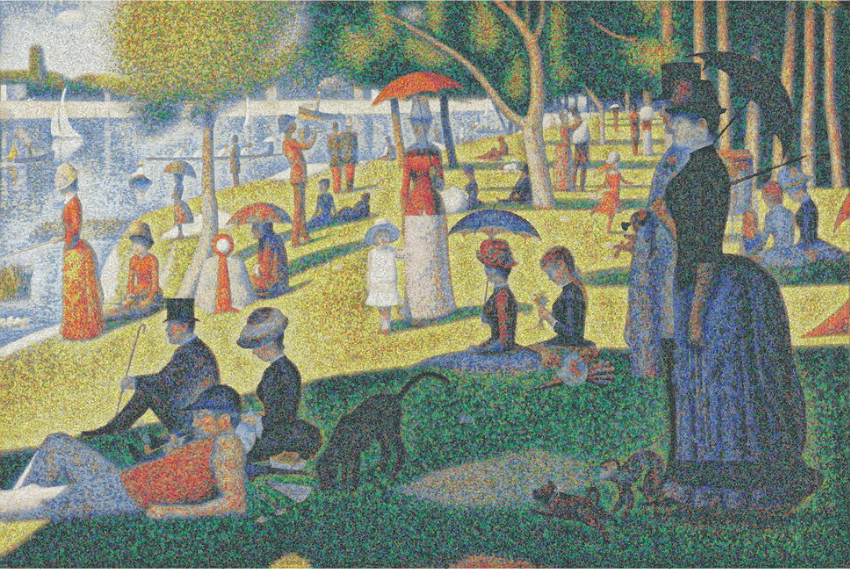
\includegraphics[width=\linewidth]{graphics/ChrisJordan_Numbers_OriginalView.jpg}
  \caption{Original view}
  \label{fig:ChrisJordan_Numbers_CloseView}
\end{subfigure}
\hfill
\begin{subfigure}{.47\textwidth}
  \centering
  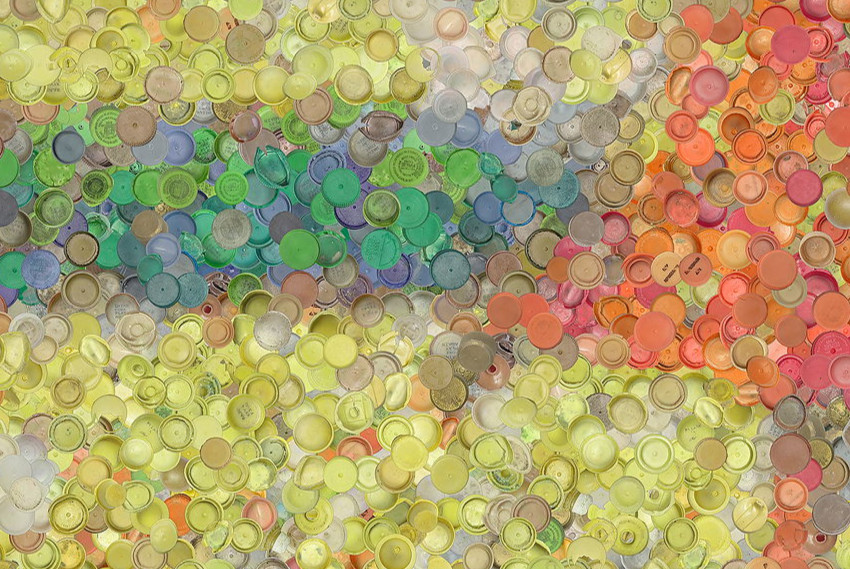
\includegraphics[width=\linewidth]{graphics/ChrisJordan_Numbers_CloseView.jpg}
  \caption{Close view}
  \label{fig:ChrisJordan_Numbers_OriginalView}
\end{subfigure}
\caption{Chris Jordan, Caps Seurat, 2011, 60x90" in one panel, and 88x132" in 3 panels}
\label{fig:ChrisJordan_Numbers_CapsSeurat}
\end{figure}

Chris Jordan creates digital photographic series that turns numbers to visuals. He provides a different way to understand the statistics and the missed reality of consumerism. He creates gigantic prints to express the numbers in a visual manner. He draws attention the global consumerism. The work reveals the reality that is hard to capture because of widespread of subject to the community and time.

\paraphrase{Caps Seurat depicts 400,000 plastic bottle caps, equal to the average number of plastic bottles consumed in the United States every minute. It is one of the pieces of Portraits of Global Mass Culture by Chris Jordan is a series of work. In this series, he revisits the statistics of modern societies.  In Running the Numbers, photographer Chris Jordan attempts to convey the vastness of modern consumption by breaking down annual statistics into more graspable quantities depicted by clever visualizations made of individual objects or groups of objects that he photographs. “There’s a disconnect that happens when we assume we know what we’re talking about when we talk about hundreds of millions of plastic bottles,” Jordan says. “I’m trying to translate these numbers from the deadening language of statistics into a visual language that allows some kind of comprehension.” Many of Jordan's works are created from photographs of garbage and mass consumption Jordan uses everyday commonalities such as a plastic cup and defines the blind unawareness involved in American consumerism. His work, while often unsettling, is a bold message about unconscious behaviors in our everyday lives, leaving it to the viewer to draw conclusions about the inevitable consequences which will arise from our habits. He recreates the most remarkable artworks with combining bits of trashes as a mosaic. Here he draw attention to the our consumerism and express them numbers that are very big to understand. All the material that we have is trash to create this pictures.}

\summary{Analysis}
In fact, the work of Chris Jordan is a reproduction of A Sunday Afternoon on the Island of La Grande Jatte which is one of the most notable works of Georges Seurat who was acknowledged as the painter of a post form of Impressionism called Neo-Impressionism. The work accepted as a well-known example of pointilizm that is a technique of painting in which little, individual dots of color are applied in patterns to form an image. This method shows similarities with mosaics of ancient times and pixels of modern times. To make an work from bottle cups with different colors can be related to painting millions of small dots on a canvas. The shape of plastics cups similar to the dots painted onto the canvas so that there could not be a better example of reproduction.

Seurat spent over two years painting A Sunday Afternoon, focusing meticulously on the landscape of the park. However, in our age, it takes only one minute to create the bottle caps that form this painting. In this respect, it reveals the point where society reached.

Visuals of Chris Jordan are like modern versions of mosaics. In the age of mass production and consumption, the most readily available material is trash. It is free and available everywhere, produced every time. Trash has different colors, sizes, and shapes. Therefore, it is a perfect material to build sculptures from them. There is a great diversity of rubbish and offers new alternatives. Nothing is missing with the physical attributes of trash to create visual work.

% Here, sculptures from trash can be added.

% ARTWORK
% TEA BAGS
% FROM https://instagram.com/silvirub/, http://www.rubysilvious.com/363-days-of-tea
\begin{figure}[h!]
  \centering
  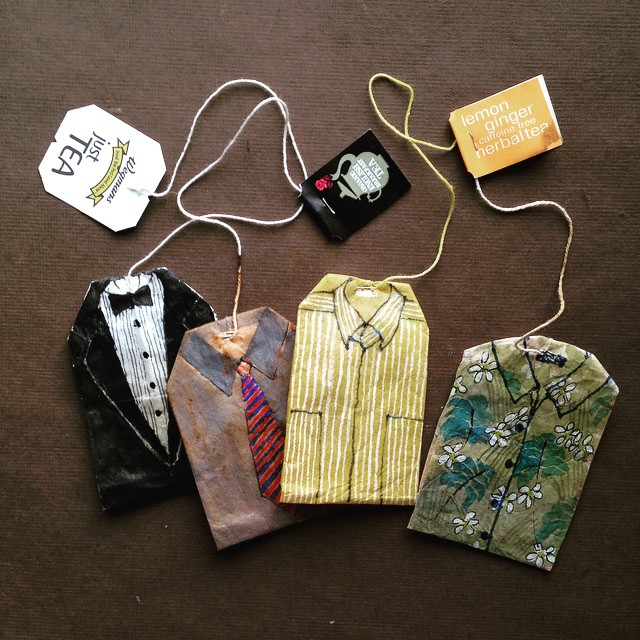
\includegraphics[height=6cm]{graphics/rubysilvious-teabag-Day169.jpg}
  \caption{Ruby Silvious, Day 169, 363 Days of Tea, 2015, Mixed media on upcycled paper tea bags, Dimensions variable}
  \label{fig:RubySilvious_TeaBag}
\end{figure}
  
\paraphrase{Visual artist and graphic designer Ruby Silvious embarked on a quirky, personal experiment, set to last for 363 days. She decided to repurpose soggy and stained tea bags as unconventional, blank canvases, just waiting to be filled with her artistic expression. The project, entitled 363 Days of Tea, allows Silvious to challenge herself by transforming the recycled material with her intricate illustrations. The artist draws, paints, and forms collages on the salvaged tea bags. This project serves as Silvious’ daily journal, allowing her to record her thoughts and feelings by creating wonderful moody and whimsical designs on little teabag papers. Every day she creates a new piece that reflects her impressions in that moment. Endeavour of re-purposing recycled and found materials.} \todo{cite website}

\summary{Analysis}
This work is for fathers day. Works of Silvious catch the important moments of days and can be as a diary (or a record of that moment and day). Trashes transformed to diaries. Trash is everywhere, already at hand. Small pieces of paper or packages are used as a canvas. 

% ARTWORK
% COFFEE CUP
% FROM http://www.gwynethleech.com/
\begin{figure}[h!]
\centering
\begin{subfigure}{.47\textwidth}
  \centering
  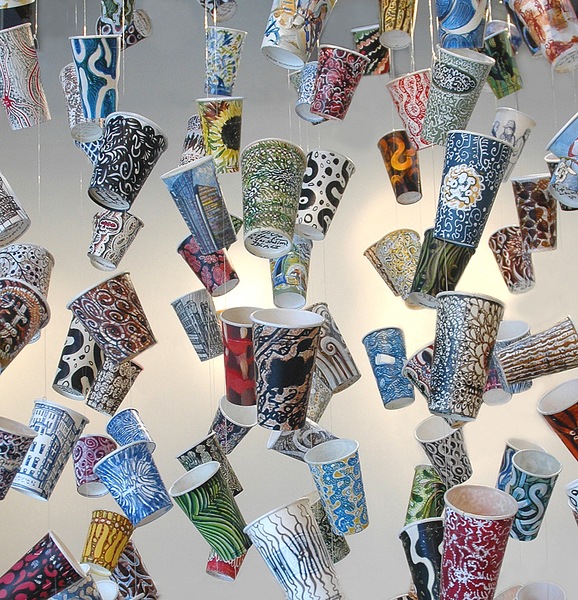
\includegraphics[width=\linewidth]{graphics/Gwyneth-Leech-cup5.jpg}
  \caption{Installation view}
  \label{fig:GwynethLeech_Installation}
\end{subfigure}
\hfill
\begin{subfigure}{.47\textwidth}
  \centering
  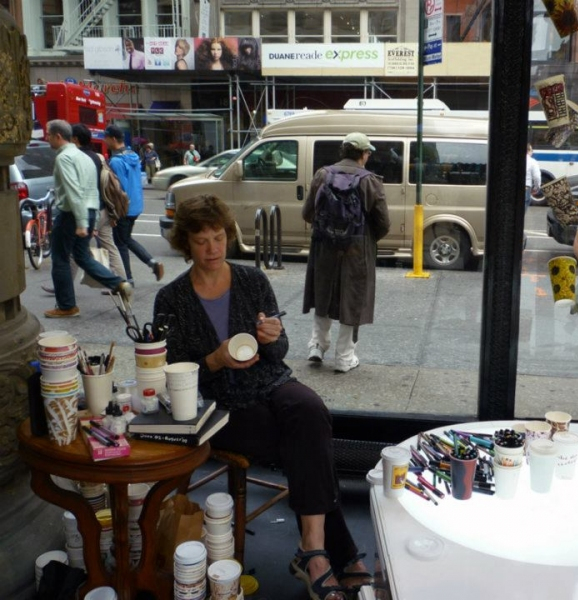
\includegraphics[width=\linewidth]{graphics/Gwyneth-Leech-cup3.jpg}
  \caption{Painting in the public}
  \label{fig:GwynethLeech_Public}
\end{subfigure}
\caption{Gwyneth Leech, 365 A Year in Cups, 2013, Mixed media on upcycled paper coffee cups, Dimensions variable}
\label{fig:GwynethLeech_CoffeeCups}
\end{figure}

\paraphrase{I began to save all of my coffee cups to use as "canvases" for making art. Transforms coffee cups that are no longer trash but a vehicle for art, ideas, conversation, and memories of a social moment upcycled from the detritus of our throwaway caffeine culture. I like my coffee or tea in a paper take-out cup. Even better than the contents, I like the used cup as a surface on which to draw and paint. Moreover, on the bottom of each one, I write the date, location, occasion and beverage consumed so that every hand-made cup artwork becomes the record of a social moment. Each cup is representing a daily caffeine break. The installation makes visible largely unconscious patterns of consumption; this is what one simple take-away purchase looks like over the course of three years, this is what would usually be thrown away. It can be seen as a measure of time gone by, of money spent, of space to be taken up in a landfill. However, as I upcycle each used cup into an artwork, it becomes the measure of other things as well: an artist's regular habit of generating new ideas, a diary of time spent with friends and colleagues, and the cumulative positive effect of doing something small and manageable every day. There are different versions of it. Paintings on paper coffee cups displayed in open window spaces. She publicly draws their cups (the cup art window installation and public drawing project were on view repeated showed at many places and date. During public drawing projects, she draws with other people. Moreover, so. Buying a beverage is a daily event for Leech (and also many people. These coffee shops all around the world. As she drinks her coffee in the public, she also publicly transforms its cup.} \todo{cite her website}

\summary{Analysis}
She is inside of glass window not white, isolated cube. Glass window provide her to be close to public space. As she drinks her coffee publicly, also paints them publicly. \todo{related with Liz Parson's argument: practice of trash to durable.} There is no difference between them, and also they should not be separated (Why? Trash, production of it, coffee cups are all experienced widespread.). By showing her practice publicly, she encourages other people in order to reconsider trash as a resource to make something. Further she is not only transforming her trash, it is everybody's trash because of everyone uses it.

These three artists mentioned here use disposable items to make their art. Their approach bring another dimension to criticize (or see) the disposable items. New things can be built from them. They can be used for new purposes.

Throwaway culture is a way of producing trash. It is a behavioral pattern, an approach to objects and commodities. Some artists develop different approaches to them. In this type of culture or behavior throwing them is a natural act and promoted. Consumption and wasting things are encouraged. On the other hand, there are examples of saving everything instead of wasting. In the work of Song Dong, "Waste Not" thousands of domestic objects are exhibited. They are owned by his mother and saved for later use. His mother lived a great depression in China, suffered from poorness. She developed the habit of saving things. After died of her husband this habit reached to extreme levels. She saves every tiny little thing. For her trash becomes an essential part of her life. In fact, it not is hard to say that preserved these things are not useless or worthless. She establishes a different relationship with these used objects.





%
%
Trash is much more than what people want to discard. Characteristic of people and societies can be understood from their produced trash.


\summary{TRASH and POTRAIT OF PEOPLE} 
Trash is a reminder of consumption and production activities. In other words, trash is bound to them, and every different of them leaves a diverse range of trash that exposes its type of action. Trash tells about societies choices. What is being left is one of the key things to realize what kind of people, society, action produce it. At one side trash is a produced thing and  What people consume is tells many things about them (their choices, possessions, etc.) \todo{ref.}. As scholars mentioned that throughout the discards of someone else many things can be understood. They are end product of people activities, and it can be traced through the discard and garbage. It is a great example of the approach to the trash is relative and changes from people to people.

\begin{figure}[h!]
  \centering
  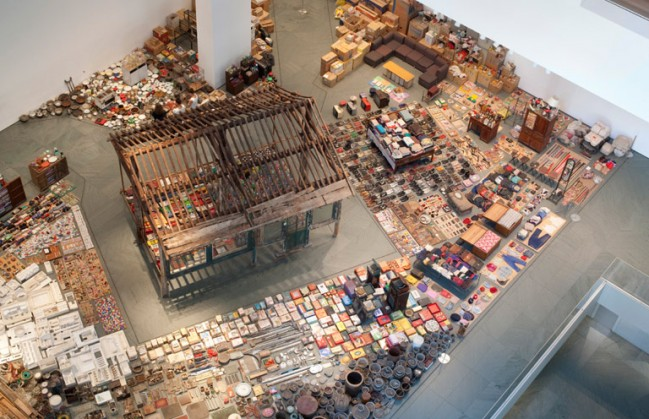
\includegraphics[height=6cm]{graphics/SongDong_WasteNot.jpg}
  \caption{Song Dong, Waste Not, 1990}
  \label{fig:SongDong_WasteNot}
\end{figure}

"Waste Not" is an exhibit by Chinese artist Song Dong that displays over 10,000 domestic objects formerly owned by his late mother, who refused to throw anything away if she could possibly reuse it. 

Song’s mother, Zhao Xiangyuan (1938–2009), was typical of the generation of Chinese who lived through the hardships of the Cultural Revolution in the 1960s and 1970s abiding by the dictum "wu jin qi yong" (waste not). As a result, all commodities owned or collected stockpiled and preserved as protection against future hardship, even in the face of improving economic conditions.

Waste Not is an installation exhibited different locations of the world. This work is a collaboration with the artist’s mother.

\paraphrase{Like many other Chinese at the time, Zhao adopted the habits of frugality and thrift in order to make the best of what little she had. Song recalls that when he was a child, "my mother always brought scraps of fabric to make clothes, because they didn't need to be purchased with the government-distributed clothing coupons." She continued to collect them even in better times because she feared that the shortages might some day return, seeing the habit of "waste not" as a fabao – literally a "magic weapon" to guard against a return to poverty.}

\paraphrase{When Song's father died suddenly in 2002 his mother suffered an emotional breakdown and her habit of holding on to things was taken to extremes, with every possible space of her tiny house crammed with thousands of domestic odds and ends. Song Dong and his sister Song Hui attempted to tidy up for her, but this led to conflict, as Zhao opposed their efforts to dispose of things that she saw as potentially useful. Song eventually came to understand that, as he puts it:}

\begin{quote}
My mother's need to fill space with daily-life objects resulted from a need to fill the emptiness after my father's death. I recognised that in this era of transition, a person could live through several different lives in just one lifetime. In the wink of an eye, one's life could undergo great changes causing deep divisions between old and young.
\end{quote}

Everything that are exhibited here is different than presented on supermarkets. They are not new and not for sale. They represents a way of life. It is common that the exhibition (museum) of famous people's possessions but this work is separated from them as showing ordinary people's objects

For most of people living in western modern societies it is unimaginable to live with all of these items together. However, for Chinese who are faced with same struggles share the emotion and  comment as "It's not [only] your home, it's my home."

Jane Alison, senior curator at the Barbican, said that Waste Not helps us to understand the reality of Chinese history and culture in the 20th century in a way that newspapers can't.

% TODO need relocation
% FROM Culture, Values, and Garbage, Encyclopedia 
%\comment{INTERACTION WITH GARBAGE. VALUE SYSTEM, DECIDING TO GARBAGE.}
%\paraphrase{"The Trash Talk project emphasizes the complex, yet overlooked, relationships that garbage and people share. In terms of their relationship to garbage, all people interact with it on two levels. One is a material connection, indicative of the physical and sensory contacts that people have with garbage. In some households, this connection begins with an individual removing an item from packaging, disposing of that item in the kitchen receptacle, placing that item and others into a larger bin, taking that bin to the curbside, and then the material connection ends. Others, including workers in sanitation plants and recycling centers, then continue a material connection with the garbage, but the material connection of the consumer and the garbage ends with the bin on the curbside. The second connection that people maintain with garbage is an ideational one. Unlike the material one, which is manifested in things that can be touched, moved, and sensed, the ideational connection operates on the level of cognition. The differentiation of an item of value from an item of trash, for example, has nothing to do with the material principles of the object. Instead, humans determine whether the object is of value or whether it is considered trash. The decision of whether an individual decides to dispose of a broken radio or to consider it an heirloom to be kept is highly subjective and rooted in the value systems of a culture." "After the item is eaten, the individual has to decide what to do with the remainder, such as the leftover package. The package might be reused, re-purposed, or recycled but, most likely, will be disposed of in the trash." \cite{lukas2012culture}}



% TODO need relocation.
% FROM Garbage in Modern Thought, Encyclopedia
%\comment{CATEGORIZATION.} \paraphrase{"Garbage is categorization, according to Susan Strasser." "In recycling programs and in places of refuse disposal, items of trash are categorized depending on their potential value, possible environmental harm, or time of decay. Consumers have become accustomed to the categories that are often applied to garbage. Many cities require people to dispose of their garbage in an orderly fashion---perhaps separating wet household waste from dry---and recycling programs ask individuals to divide their recyclable items into sets (such as plastic, glass, aluminum, and paper). Garbage is an illustration of how humans use mental categories to order the material world." \cite{lukas2012garbage}}

% TODO need relocation.
% Garbage is universal.
%\comment{NO VALUE, UNIVERSAL} \paraphrase{"According to John Scanlon, garbage is indicative of a separation of the world---the desirable from the unwanted. Michael Thompson uses the riddle of the rich and poor person’s approach to snot (one keeps his in a handkerchief, the other disposes of it with a tissue) to underscore the curious ways in which garbage is connected to the issue of value. While garbage is universal---all societies, extinct and extant, have produced or produce garbage--- the conditions under which garbage is understood are culturally determined. Many non-Western societies attach a much greater value to items after they are discarded. In the United States and many other nations, garbage often results not because something no longer has utilitarian value but because the item in question is defined as something of no value. Thus, garbage is not only an objective condition of material culture, but also a subjective one of mentalist culture. People define what is trash and what is valuable." \cite{lukas2012garbage}}





%
%
\summary{Garbology}
Garbology is a study of waste as a social science. Applying methodologies of archeology to the human debris. 

\paraphrase{Weberman infamously used techniques of what he deemed garbology to uncover what he saw as the essential nature of people. He once said, perhaps indirectly referencing Jean Brillat-Savarin’s quote about food, \quotes{You are what you throw away.}" \cite{lukas2012garbage}}

% Garbology, from Encyclopedia, Abhijit Roy
\paraphrase{The field of garbology involves the study of refuse and waste. It enables researchers to document information on the nature and changing patterns of modern refuse, hence assisting in the study of contemporary human society or culture. According to the Oxford English Dictionary, the term was first used by waste collectors in the 1960s. Weberman popularized the term in describing his study of Bob Dylan’s garbage in 1970. It was pioneered as an academic discipline by William Rathje at the University of Arizona in 1973.}\todo{ref.}

\paraphrase{The work of archaeologists such as William Rathje and Cullen Murphy has offered significant insights into the relationship between archaeological artifacts and garbage, exploring the function of trash as a resource for understanding the cultural and social practice. At the same time, thinkers such as Zygmunt Bauman and Giorgio Agamben have shed light on the fate of the human being as a wasted or discarded element in discourses of socio-political hygiene. (from Trash Culture)}

\todo{transition required.} With the help of mentioned understanding of trash, what can we see the work of arts?

\begin{figure}[h!]
  \centering
  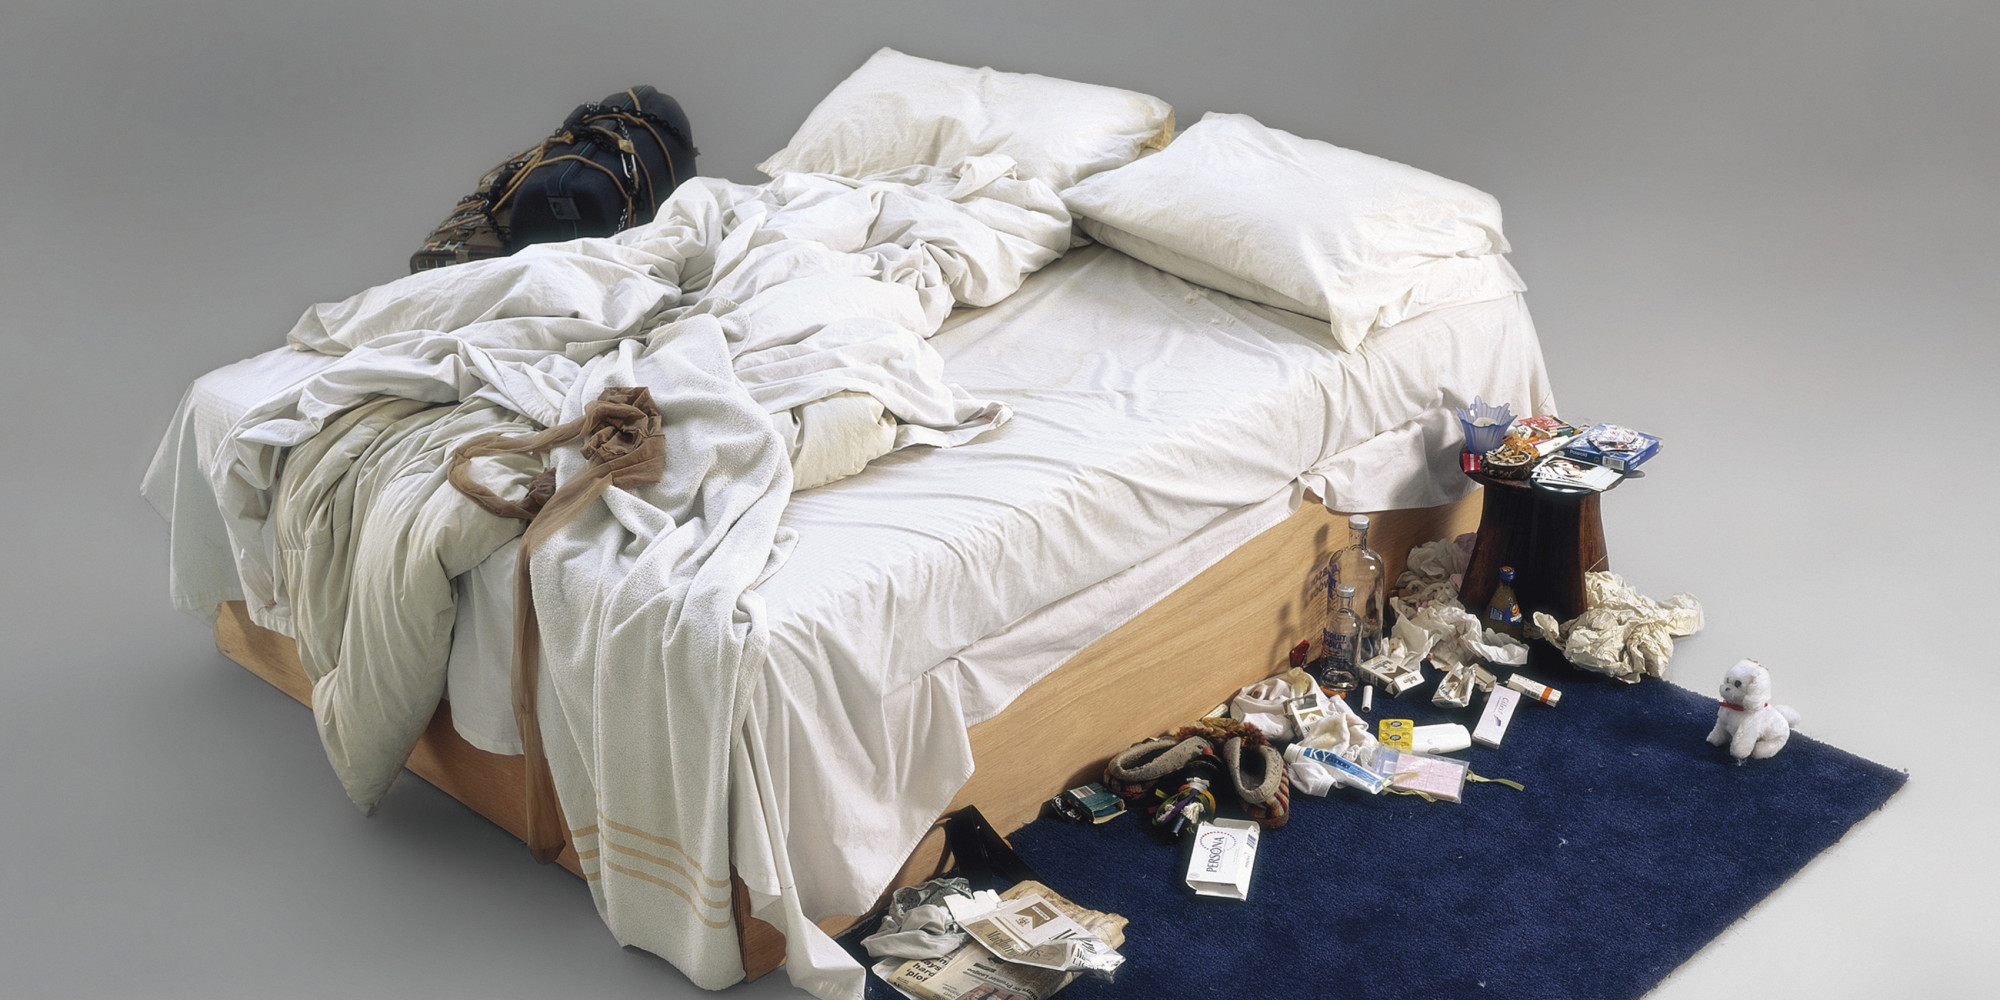
\includegraphics[height=6cm]{graphics/tracey-emin-my-bed.jpg}
  \caption{Tracey Emin, My Bed, 1998}
  \label{fig:TraceyEmin_MyBed}
\end{figure}

Tracey Emin puts her private life to the public. The work, which Emin now describes as a portrait of a young woman. Around her, there are pieces of junks speared all over the room. We can understand from her junk what type of life she has. We enter the world of the artist through her trashes.

% From wiki
Every detail of her private life is presented through her bed. The idea for The Bed was inspired by a depressive phase in the artist’s life when she had remained in bed for several days without eating or drinking anything but alcohol. The sensation of depression leading to disarray and detritus is not wholly unfamiliar to many people, and The Bed therefore enforces the communicative power that Tracey Emin seeks with her work. The artwork generated considerable media furor, particularly over the fact that the bed sheets were stained with bodily secretions and the floor had items from the artist's room, such as condoms, underwear with menstrual blood stains, other detritus, and functional, everyday objects, including a pair of slippers. The bed was presented in the state that Emin claimed it had been after languishing in it for several days; at the time she was suffering suicidal depression brought on by relationship difficulties.

It is a realization what she did during her depression time. It perfectly represents her condition during days. It can be understood that trash is part of our life. Things that are exhibited in this work are part of her action. She created them and later through them in the mind of people the condition and life of Tracey Emin are recreated. 

% Independent http://www.independent.co.uk/arts-entertainment/art/reviews/tracey-emins-my-bed-at-tate-britain-review-in-the-flesh-its-frankness-is-still-arresting-10144882.html
You can interpret it as an uncompromising self-portrait of a woman at a time of emotional trauma – or as a turbulent still life – but it is still a bed and all that a bed symbolizes and encompasses: sleep, sleeplessness, sex in all its manifestations, birth, death and dreams.

Beds meaning also are not same for everyone. It is not just for sleep. Especially for the ones that have small rooms and spaces bed becomes a life space. I have also experienced such a thing at boarding school and university dormitory for total my eight years. Having tight space sometimes bed becomes a place for studying and reading. Sometimes it was used to dry the clothes. It is more than sleeping and provide place for other activities.

% Aslan yattigi yerden belli olur.





%
%
\section{Zizek's Approach to Rubbish}
Last decades there is an increasing attention the ecology and rubbish. Global warming is one of them, plastic pollution on the oceans also is part of it. These types of news and talks increasingly find a place on media more and more. At this stage, Zizek comments on ecology and trash conversely.

\paraphrase{In the late twentieth century, in the context of increasing environmental awareness, this consciousness has altered yet again, and waste has ‘been revalued and recoded from rubbish to recyclable resource, it has moved from the bin to the compost heap, it has insinuated itself into our lives in different ways and with different effects’ (Hawkins 2006: 5).}

In the documentary film Examined-life Zizek dressed as a sanitation man discusses ecology in the middle of a dump in London. His part starts with these sentence: \quotes{This [dump] is where we should start feeling at home}. The place where he talks is a site for depositing people's excess and unwanted material. It is a place of out of sight.

He draws attention that the thrown out garbage only disappears from people's living environment. Particularly discarding it is an action of escape from the unwanted. However, it still exists in reality and waits at somewhere else. In other words, it does not disappear, moves away.

According to Zizek, the way of approaching ecology is problematic in current societies because of accepting nature as a balanced, and harmonious. He claims that it is ideological in the sense that "wrong way of thinking and perceiving reality". The meaning of ideology is here mystification of real problems. He claims that one of the key mechanism of ideology is temptation of meaning. In other words, people search for meaning when a terrible event happens in order to make it easier to accept. He opposed the notion of the existing world is in the best possible state and that humans disturb nature. According to him, nature is not an organism in balance that humans exploit, but rather a series of "unimaginable catastrophes" by asking the question what type of disasters would happened on the earth to compose oil that is a significant source of energy. Zizek asserts that ecology will slowly turn to a conservative ideology that is a kind of an unquestionable highest authority. Its voice is like "Do not mess with D.N.A. Do not mess with nature". In the light of these arguments instead of talking from an authoritarian high ground, he suggests that to find poetry and spirituality in the dimension of rubbish people create. He thinks that that is the true love of the world by asserting that "love is not idealization." Therefore, that is the reason why he thinks that a dump is a place that people should accept it as a home. 

In the light of Zizek's arguments ecology is not an appropriate point (or enough) to approach trash. He points out the need for the new approach to trash. This new approach should not idealize it. At this point where the practices of art gains importance to establish new understanding of trash.

Not every act of transforming trash is not related to ecological concerns. Artists are not trying to save the planet earth. Beyond ecological concerns, they are attempting to find new ways to look and live with trash. 

Some artists turned to trash into site-specific sculptures that are more than trash heap after their intervention. Not discarding but bracing our attitudes turned them to a something that worth it to watch and think about it. (Converting what we create harmonious with the existing system. Because it is not possible to think that nature will live harmoniously with what we created. The more reasonable idea will be we will live harmoniously with what we create.) Turning trash to things that can be lived together.

Beyond the ecological problem, there are different sides of it. Different readings can be added to the topic. Adding spirituality and new aesthetics dimension to the topic. 

The idealization of nature is problematic. Loving nature is loving trash. Live with trash. Do not see it as trash. Then the question is How to love trash? How to live with trash? Think beyond the common perception. Do not consider it as abject, disgust. Can live with our trash enrich (our perceptions, abilities)? How not to see them as trash and useless? Can it be possible with art?





%
%
\section{Rubbish Theory}
Objects have a lifetime similar to humans, and they do not remain same through that time. They move around, and their value, usage, location change constantly. During their lifetime objects may circulate different markets and values systems such as economic, social and aesthetic. Especially these cycles have picked up speed with the advent of consumer culture. For instance, most recent technological gadgets become obsolete within two or three years. Firsthand, secondhand and even trash is exchanged among not only people but also countries. People from other cultures and understanding interpret objects differently. They often are not aware of their initial and intended usage. They find new original purposes and meanings. Therefore, objects turn different items in their hand. Anthropologist Sidney Mintz (as cited in Susan Strasser) writes that "I have seen automobile bearings fashioned into portable vulcanizing kits; bits of toothbrush handles used as 'jewels' for rings, and ordinary tin cans turned into simple kerosene lamps." As it can be understood that objects function and value are transformed by relocation and revaluation of objects from one place to the other or one discipline to another. 

In ‘The Social Life of Things’ Appadurai (1986: 3) highlights that "commodities, like persons, have social lives." As such, Kopytoff wrote, the biography of an object was considerably similar to that of a person: occupying different positions, leading diverse careers in the course of different periods between a beginning and an end, being defined by different regimes of value that are both economically and culturally inscribed. Appadurai focuses on the "commodity potential" of things and asserts that "things can move in and out of the commodity state, that such movements can be slow or fast, reversible or terminal, normative or deviant" (1986: 13). However, one can ask that what are these commodity states and does anything exist between them? Thompson’s Rubbish Theory fills this gap.

Thompson observes the creation and destruction of value in man-made objects, cultural artifacts, and ideas. He notes how an object’s economic and cultural value diminishes over time rendering the objects worthless or redundant and how others value increases overtime. In his notable Rubbish Theory, he declares three object states; transient (normal state, decreasing value, circulating), durable (permanent, increasing value, removed from circulation) and rubbish (zero value, will be destroyed or reinvested for economic and social value). The transient represents the common state of objects that are lessening in value and have limited life period. A used car can be an example of transient state. On the contrary, the durable objects increase in value over time and have (ideally) infinite life spans. Antiques and objects in museums can be an example of durable. This theory gives rubbish a key role between transient and durable. 

% TODO Bu nereden
Rubbish is, by definition, an object that is not or is no longer, owned by anyone, which falls outside all categories of economics, culture, and social control. As one of many things on the garbage heap, a discarded object even tends to take on a negative value as something unsanitary, dangerous. The socially constructed value of the object has shifted over time from its finite life span of usefulness and meaning to a timeless and valueless of socially sanctioned rubbish. 

The potential of the discarded thing also relies on its status as a thing approaching a zero point of value. In other words, it has reached a point in transition between the world of the functioning, the useful and visible, and the realm of the invisible, the non-functioning and empty. As Michael Thompson’s Rubbish Theory suggests that rubbish is both ready for the disappearance and yet ripe for reinvestment, reinterpretation or revaluing. Trash as a state of being flexible is ready to transformation.

Similar to Žižek's claim that is "trash does not disappear", Thompson notes that "in reality ... [trash] just continues to exist in a timeless and valueless limbo, where, at some later date (if it has not by that time turned, or been made, into dust) it has the chance of being discovered."

Thompson argues that rubbish represents an important possible ‘in-between’ category in a ‘region of flexibility’ which is not subject to the same control mechanisms of the valuable and socially significant categories of transient and durable. Therefore it ‘is able to provide the path for the seemingly impossible transfer of an object from transience to durability’ (1979: 9) he further suggests that ‘a transient object gradually declining in value and in expected life span may slide across into rubbish’ (1979: 9) where it has the chance of being re-discovered, brought to light or cherished once gain. Figure X demonstrates the possible paths an object may take (from transient to rubbish and from rubbish to durable).

\begin{figure}[h!]
  \centering
  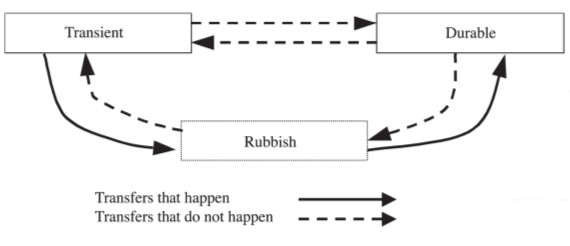
\includegraphics[height=4cm]{graphics/rubbish_theory.jpg}
  \caption{Thompson’s Rubbish Theory}
  \label{fig:rubish_theory}
\end{figure}

The transitions between these states defined as follows: from transient to rubbish (transient -> rubbish) and from rubbish to durable (rubbish -> durable). 

To illustrate rubbish theory the series of compression by French sculpture César can be analyzed in the context of it. His early work is composed of soldered and welded metal as well as junk materials. In 1960, Caesar discovered the hydraulic press that is capable of compacting scrap metal (especially car bodies) during on a visit to a scrap merchant in search of metal. He admired from the hydraulic crushing machine in operation and started to experiment with it in his sculptures. The machine is used to compress the metal items in order to gain from space. His first three automobile compression exhibited at Salon de Mai in 1960 and bring him a supportive fame. Later Viscountess Marie-Laure de Noailles who is important figure of these ages, gave him her Zim model car to compress. It is 
% http://www.sothebys.com/en/auctions/ecatalogue/2015/art-contemporain-pf1515/lot.6.html
"a revolutionary artistic gesture then, but also a strong political gesture, right in the middle of the Cold War; César having chosen to lash out against a Zim, a jewel of the Soviet automobile industry commissioned by Khrushchev at the beginning of the 1950s to compete with the Cadillac." Additionally car was one of the most desired possessions of people in 20th century. Through the eyes of rubbish theory it is a transient object and after the intervention of artist, it is transformed into an artwork that preserved in the collection of Museum. In other words, it switched to durable category by interestingly trashing it. 

\begin{figure}[h!]
  \centering
  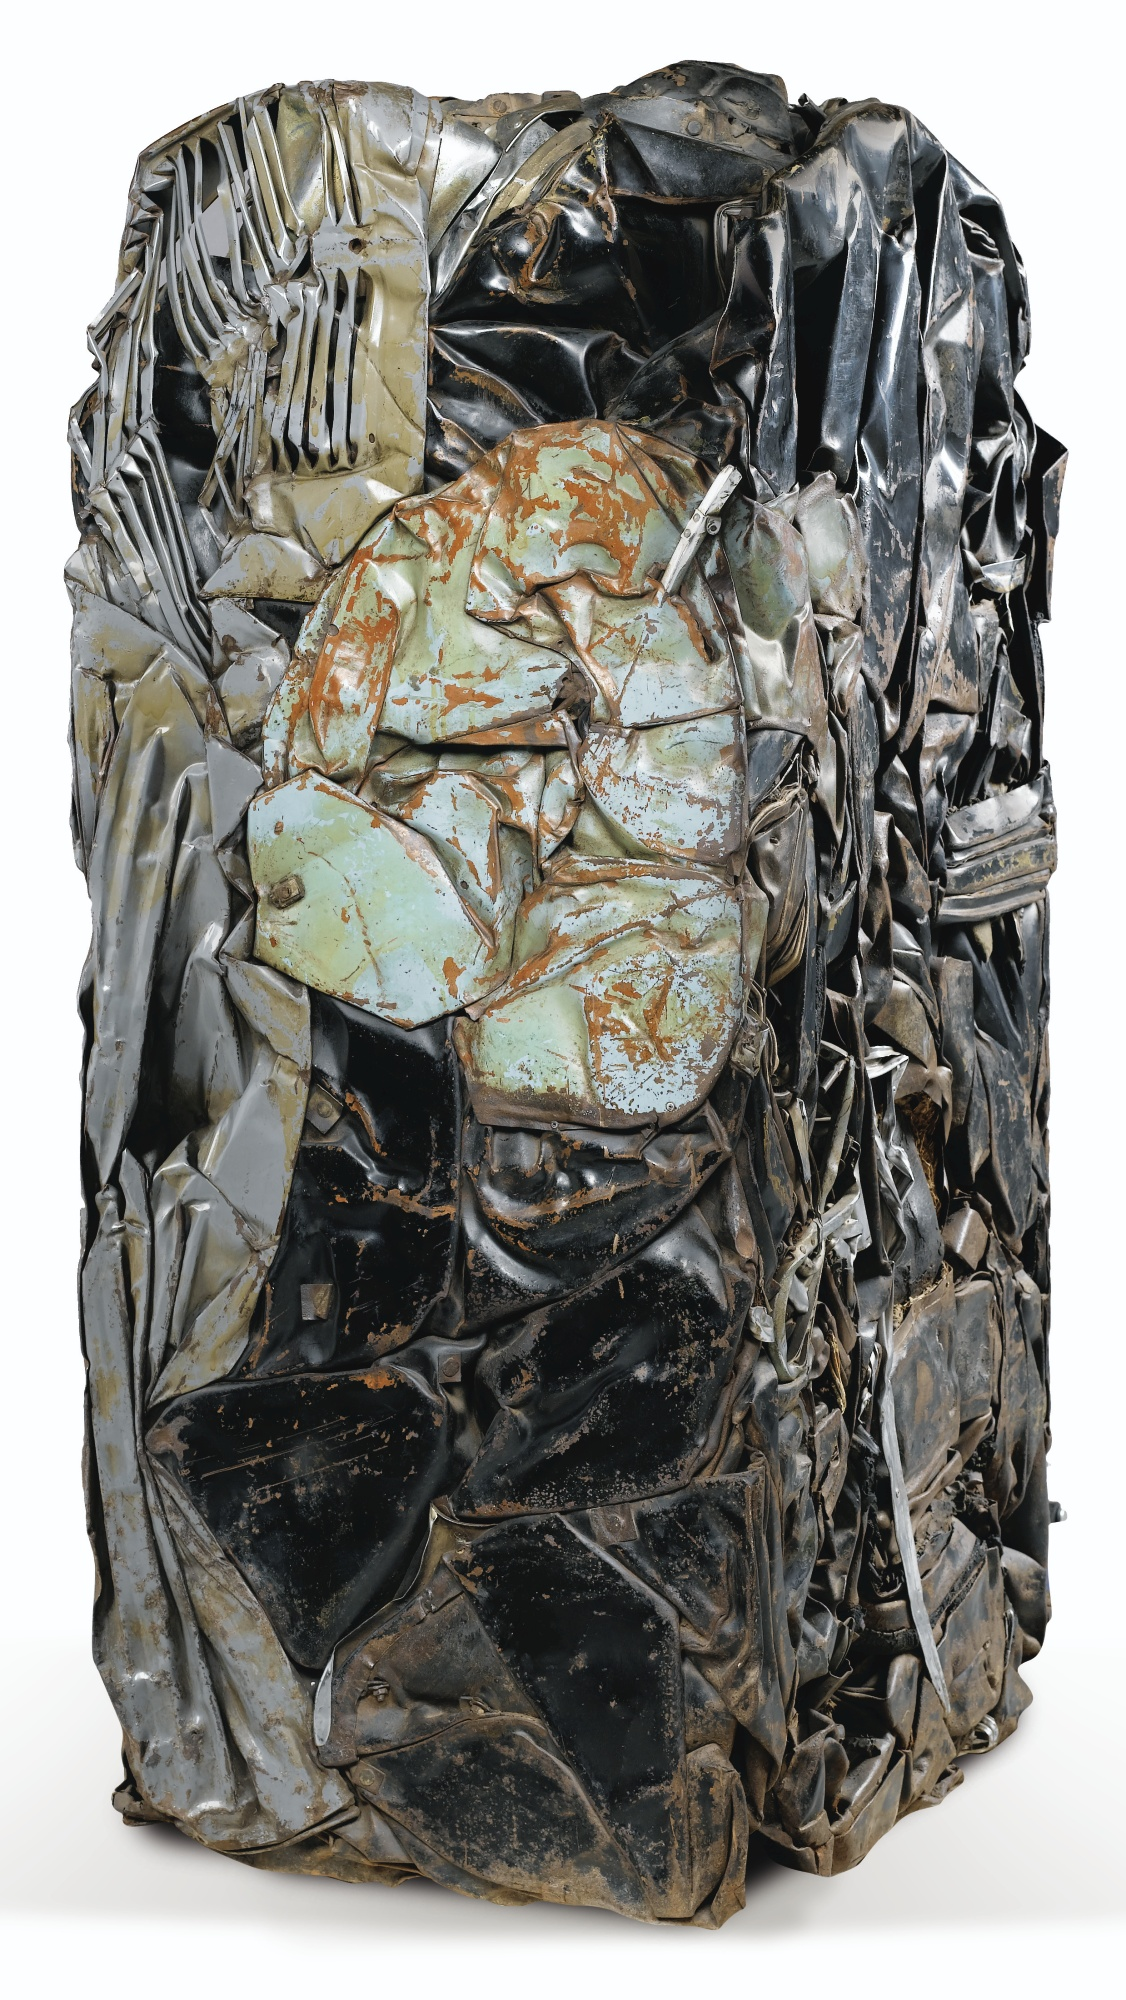
\includegraphics[height=6cm]{graphics/Cesar_Zim.jpg}
  \caption{César, Compression Zim, 1960-1961, 157 x 82 x 64 cm}
  \label{fig:Cesar_Zim}
\end{figure}

Although Thompson is quite successful describing states of objects, claimed transitions between states in the theory have some problems. Thompson label some transitions as possible and the others as impossible. He only allows movement of goods from transient to rubbish, and from rubbish to durable. Movement in the other directions, from durable to either transient or rubbish, does not exist in this system. However, Duchamp's notable ready-made "Fountain" is one of the examples outside of the defined transitions.

\begin{figure}[h!]
  \centering
  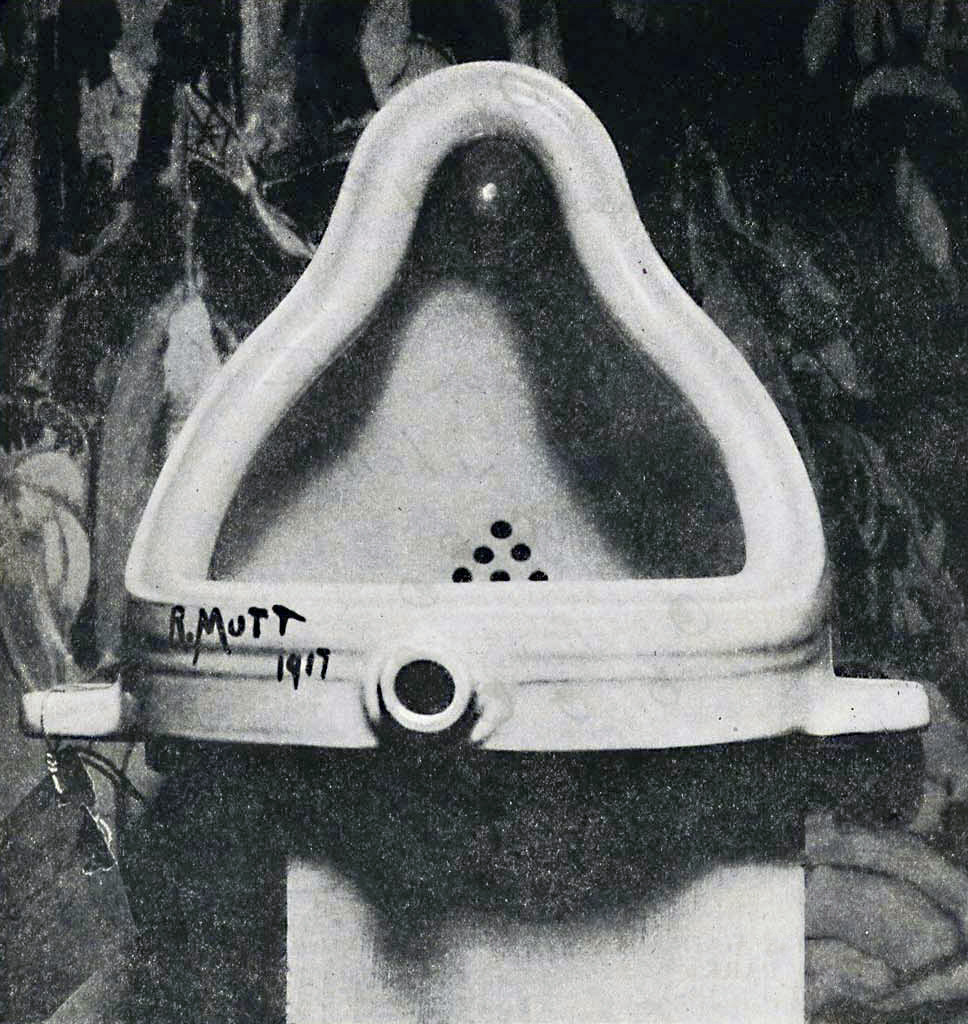
\includegraphics[height=6cm]{graphics/Duchamp_Fountaine.jpg}
  \caption{Marcel Duchamp, Fountain, 1917}
  \label{fig:Duchamp_Fountaine}
\end{figure}

Fountain is a 1917 work produced by Marcel Duchamp, who is notable member of provocative Dada movement. The piece was an industrial porcelain urinal, which was signed "R.Mutt". Submitted for the exhibition of the Society of Independent Artists, in 1917, Fountain was rejected by the committee, even though the rules stated that all works would be accepted from artists who paid the fee. It is considered one of the major artworks of the 20th century because of challenging the existing understanding of art. Duchamp used already existing fabricated ordinary urinal to express his ideas by challenging existing way of art making which requires efforts of the artist. It forces to the limits of the language of art and perception the art. To understand his works requires shift inside of the peoples mind. For him, the idea is important rather than the object. He also criticized the position of artist by signing urinal as "R.Mutt" who is actually not exist. In the editorial The Blind Man summarized this work as follows: "Whether Mr. Mutt with his own hands made the fountain or not has no importance. He CHOSE it. He took an ordinary article of life, placed it so that its useful significance disappeared under the new title and point of view – created a new thought for that object.\todo{ref}" To debate all the aspects of this work is not possible with the scope of this thesis. However when it is analyzed through the frame of rubbish theory, urinal a transient object turned to durable objects that are exhibited by the intervention of artist. Urine titled as "fountain" is still functional and have a place in the market. In another word, it is not rubbish.

\todo{bir conslusion lazım buraya.}

% TODO move to conclusion.
%Rubbish theory suggests that value emerges through people ways of seeing, and their category membership determines the way people act towards them. Similar to X (as indicating that scholars agree on this argument.) 

% TODO move to conclusion.
% \paraphrase{Michael Thompson’s study Rubbish Theory elaborated an understanding of rubbish as part of a flexible and shifting system of value construction, underlying notions of innovation, creativity, and social status.} \todo{ref. from Trash Culture} \paraphrase{It is clear that one man's rubbish can be another man's desirable object; that rubbish, like beauty, is in the eye of the beholder \cite[97]{thompson1979rubbish}.}





% TODO relocate
% From "Trash Moves On Landfills, Urban Litter and Art" by Maite Zubiaurre
%\summary{Moves} 
%\paraphrase{Below part explains journey of trash in different steps/stages. Object moves and trash also moves. How is it life of trash? This part explains life of trash. How does it intersect with other people in which places? This part also can be understand by pointing out different part of it with detailed explanation. For example an artist collect from trash from streets and the other one goes to the (For example Vik Muniz) landfill. In other words there are different places to touch on trash. Every place generates different story? Or to understand it more deeply it covers different part of it. Or provides ideas about it. Lots of people touches it from philosophers to artist. Also in the later parts it draws attention to them.}

% TODO relocate
%\summary{Moves}
%\paraphrase{Trash moves, all the time. It becomes a steadily growing heap of clutter behind closed walls, accumulates and festers under tight lids, travels from a small trash can in the kitchen to a large one on the curbside, joins other people’s rubbish when the garbage truck arrives, drives to the transfer station, where it circles around on conveyer belts, bids farewell to recyclable or composable goods, is loaded (if declared useless: the ultimate trash) into yet another garbage truck, or barge, or even train, until it arrives at its final destination: a sanitary landfill. Even in the landfill, it does not remain still. Monster "waste handling dozers" move rubbish around, compact it and press it against the soil. More importantly, they incessantly “sculpt” refuse with their huge shovels and caterpillar wheels, making sure the garbage mound does not tip over to create a fetid avalanche. When night falls, and the trash load of the day finally disappears under a thick layer of mud, detritus still moves: once underground, it settles differently, and decomposes at a different speed, thus continuously altering landfill topography: where there was an even plateau, now there is an abruptly descending slope, and a valley; and where there was a perfectly smooth road, now there are deep crevices in the pavement. This is how trash moves. But\ldots who moves on trash? In the United States, it is mostly big-wheeled machines, an industrious army of giant yellow insects busying themselves on a heap of rubbish. In Latin America, it is mostly people. People who hand-pick garbage, who build their shacks on densely compacted trash layers, and who, day in and day out, eagerly throw themselves into the boisterous cascades of fresh debris falling from garbage trucks. In many of the garbage dumps around the world, scavenging becomes a steady job. \quotes{Garbage properly \quotes{stored} and put away brings peace of mind, as do corpses boxed and buried, or criminals confined to a cell.} And thanks to Art: for Art shows how trash--even the one that stops moving, and particularly the one that lies squished, squashed, and weathered, almost fossilized, on the ground---has the potential to move: to move us, that is. (through the works of Filomena Cruz's photographic series “Road Kill”)}

% TODO relocate
%\summary{Categorization of waste} 
%\paraphrase{Douglas argues that our classification of dirt lies not with what objects are but where those objects are. (Think that the transformation process. Previous argument support that the transformation of trash is possible by changing the place of them. In other words removing them from landfill and waste bins to the book selves accomplish to transform trash.) ‘Dirt’, writes Douglas, ‘is the by-product of a systematic ordering and classification of matter, in so far as ordering involves rejecting inappropriate elements’. For Douglas dirt is a spatial problem, a question of not what stuff is but where it is.} \todo{Reference, (Waste by William Viney).} 

% TODO relocate
%\paraphrase{“Dirt”, writes Douglas, “is the by-product of a systematic ordering and classification of matter, in so far as ordering involves rejecting inappropriate elements.” Dirt is only dirty in certain places, when it is out of its correct position. Just as faces, for example, is considered dirty when it is in our kitchens but not when it is in our bodies, so it is that our classification of waste depends on the location of objects.}  \todo{Reference, (Waste by William Viney).}

% TODO relocate
%\paraphrase{Waste is “matter is out place”, a definition first given by Lord Palmerston in the mid-nineteenth century and incubated by the British anthropologist Mary Douglas, in her book Purity and Danger.}

% TODO relocate
%Trash is something that is out of sight, out of mind. Paid little attention to them and only catches attention when it is in wrong place. It is an unexpected object for people. Therefore transformation of it can create powerful and suprising effect onto the people. 

% TODO relocate
%\paraphrase{Thompson comments that we only notice rubbish when it is in the wrong place, and highlights the embarrassment and anxiety that mis-placed rubbish, or rubbish which has found its way in to the wrong place can cause ‘Something which has been discarded, but never threatens to intrude, does not worry us at all.’ (1979: 92) but rubbish in the wrong place is ‘emphatically visible and extremely embarrassing’ (1972: 92). (Further there is similar analogy at Waste and Want. The author give the example of shoe and claim that thrash is relative. The shoe on the dinner table is something disgusting but in the foots is not at like that.) Rubbish objects are things that are no longer used or loved or cared for and often no longer seen. Rubbish objects linger on the periphery of our lives, in the back of the drawer, bottom of the wardrobe or cupboard, corner of the garage or garden shed gathering dust. (Summary From Liz Parsons.)} 









%
% TODO move it to the art chapter and discuss it with the found photos.
%\subsection{Rubbish Theory in Practice: From Rubbish to Durable}
%\paraphrase{In rubbish theory beyond the objects states how it happens transition of objects in practice is missing and Parsons fills this gap by claiming that transition from rubbish to durable are possible with finding objects, displaying objects, re-using objects \cite{parsons2008thompsons}.} (finding paper, transforming to notebooks and giving away them to create an opportunity to be displayed different location and times.) 

%Three such sets of practices are explored below, they include: finding objects, displaying objects and transforming and re-using objects. It is argued that each of these sets of practices changes the way we view an object moving it from being seen as a ‘rubbish object’ of no value to a ‘durable object’ of increasing value.

%\textbf{Finding Objects:} One key way in which objects may slide from the category of rubbish to durable is through the act of finding. Indeed, Gabriel and Lang (1995) include the ‘Consumer as Explorer’ as one of many possible consumer identities. What, then might one mean by ‘the find’? Ultimately the find relates to discovery, and suggests that something has been otherwise overlooked, ignored or hidden away. The find may not involve objects which are new to us, it is possible to find some of ones own items if they have been hidden away long enough in an attic and thus made strange to us. The concept of the find also suggests that the found object has some qualities that others (or indeed ourselves) have in the past overlooked, as such it is closely related to ‘bringing to light’. The find may be extended to embrace features of objects as well as objects themselves. This directs us to their ‘potentialities’, objects may have been there all along but we’ve suddenly found them to be useful, likeable or beautiful. It might be that some aspect of them has simply been brought to our attention. Equally, as discussed below in relation to transforming objects, we may make alterations to objects which bring out their potential. The transition from thing of little or no value (rubbish), to thing of value (durable) can result form a relatively minor shift in the way we see something.





%****************************************
% Theoretical Analysis of Found Object
% (Summary From Paul M Camic.)
%\summary{Theoretical Analysis of Found Object}
%\paraphrase{As a species Homo sapiens has been gathering and collecting objects for thousands of years. Food, clothing, weapons, fuel, animals, and plants are the more obvious items, but visually pleasing objects, things that arouse curiosity, and shapes that stimulate the imagination have also been sought. The search for “things,” collecting them (Humphrey, 1979), and the need to embellish and make the ordinary special (Dissanayake, 1988) have been essential parts of the evolutionary process of human development (Bettinger, 1991; Dissanayake, 1992). For example, many early cave drawings occur around a natural feature within the cave such as a projection or indentation (Bahn, 1998; Lewis-Williams, 2004), making these natural features potentially comparable to found objects in modern and contemporary art (Read, 1930). When early prehistoric eople recognized a cave’s natural feature as a “found object” and incorporated it in a picture, it is possible that the natural feature took on a higher value than if left alone, thus adding to the value of the object on the cave wall. Once found and incorporated in paintings and drawings on a cave wall, it is possible that these protrusions and indentations became objects that functioned symbolically.}

%\paraphrase{In contemporary societies, people seek objects to adorn bodies, decorate homes and gardens, and personalize places of work (Menzel, 1994). Seeking and finding objects, whether in vast Asian cities, remote African villages, or the high streets of Europe and North America, have become part of daily life for millions of people. Although most of these objects are purchased new in shops or online, many others are preused items, castoffs, or trash found in back alleys and country lanes, dumpsters, and rubbish bins or purchased cheaply in flea markets, garage and boot sales, and in shops catering in previously owned goods. Some individuals have chosen to salvage objects out of economic necessity, as depicted in Jean-Francois Millet’s 1857 painting The Gleaners and by Agne`s Verga’s 2002 documentary film Les Glaneurs et la glaneuse, whereas others have done it for a range of other reasons, including a desire to rescue them (Belk, Wallendorf, \& Sherry, 1989). These “other reasons” pose an opportunity for researchers to better understand why people voluntarily seek society’s discarded material objects and how they make use of them. A form of cultural reuse, the process of salvaging and using found and second-hand objects has potential implications for \ldots}
%........................................





%\textbf{Displaying Objects:} by displaying objects in home, fashion etc. (This is not a strong category.) Maybe publicly exhibiting them. 

%\textbf{Transforming and Re-using Objects:} These transformations may involve creating new uses for old things to fit in with contemporary lifestyles. Transformations may also involve the modification or updating of objects through painting, alteration or repair. Transformations may not only be based around creating new uses but also creating new looks. The re-use of objects also creates value for things that otherwise would be allowed to slip away (or slide terminally into the rubbish category).





%
% TODO Move to Conclusion.
%Trash has archaeological value. It reflects our habits. It is like a mirror. Can not be sepereted from their producers.

%Ecological perceptions have problems. In modern socities trash seen as an ecological problem. 

%Moving nature of trash/objects. Objects value/state is not static open to intervantion, has potential to be reconsidered. Their place shift in the society. Classification is the main key, being trash is not related with the object property. It is about perception the trash.

%First part analysis trash of disposable items and the works of art that looks differently to these trash. Whose trash? Which trash? Answers these questions. It displays common approach to the trash. Artist reflection to them. When we look at personal level (previous one is general one) discards tells us about our activities, possessions, preferences etc. They can be viewed as portrait of artist and us.

%Firstly trash is created (by the throw away culture). Even if there is counter argument about it, the focus is disposable items and their amount is very high. After generating mountains of garbage the approach of zizek introduced. What to do this garbage see. He claims that we need to find a way to handle it. Find aesthetics and other things. Learn to live with the trash.

%Zizek points out wrong opinion about ecology among the society. Stacking trash outside of living space is not the solution.

%Later rubbish theory and relative approach to the trash. Trash is not static. Objects are not static. It related with the perception.

%Thompson thinks that the switch only occurs when all the value to the given object is removed. To gain a new value, meaning and purpose it must be exit from previous system.  Changing the context can only be possible first rubbishing them or loosing all value.

%Thompson and Zubiaurre say trash moves amoung various range of value systems. 

%Zizek says you must find a way of loving your trash, or a way of living with trash instead of idealization of nature and waste. Purification is not suggested by him.

\chapter{TRASH (IN) ART}




% Epigraph
\begin{singlespace}
\epigraph{One day, in a rubbish heap, I found an old bicycle seat lying beside a rusted handlebar, and my mind instantly linked them together. I assembled these two objects, which everyone then recognized as a bull’s head. The metamorphosis was accomplished, and I wish another metamorphosis would occur in the reverse sense. If my bull’s head were thrown in a junk heap, perhaps one day some boy would say, \quotes{Here’s something that would make a good handlebar for my bicycle!}}{\hfill ---Pablo Picasso, \textit{Trashformations}, 1998}
\end{singlespace}





In this chapter, I question the purpose and meaning of using trash as a medium in the artworks. The reasons and motivations of artists who use trash will be elaborated. The artists who use discarded items in their work will be analyzed in the light of arguments discussed in the previous chapter. Here, the main question is why artists select to use society's debris rather than fresh items. Hence, my research will focus on the place of trash in the world of art by looking at different methods and approaches. The scope of this research is Started from masterpieces and founding works, and continued with recent examples of artworks.  

% Çöpün sanatta kullanılmasının temelleri arastirilmakta.

% Ben bölümde aslında çöpün sanatta nasıl yer aldığına bakıyor olacağım. İlk kim kullanmış nasıl kullanmış. Sonrasında hangi anlamlarda kullanılmış. 

Firstly I look at how artist started using objects that are not produced by herself/himself and with the purpose of making art. Early works are notable and founding ones that open new dimensions to reconsider objects and their meaning. Further, they extended the ways of art making and the language of art. Therefore, it is important and necessarry to analyze them. In other words, I first look at the foundation of using non-art objects in the art making. Early examples are analyzed and how they evolved over time is explored. I try to find out how they affected successor artist.

Secondly looked at some examples of contemporary works (or works from recent history). In particular, I try to capture the current approaches on trash. Several methods and genres are explored.  Lastly focused on the inspiring documentary of Agnes Varda, The Gleaners and I which provides a general picture of the subject.





%
%
\section{Root in the Art History}
Using trashed objects in making art can be examined with the use of non-art objects in modern art. In other words, some artist started using objects in different scope beyond their intended purpose or intended meaning and function in their modern artworks. They develop their artworks by using paper and other stuff by pasting (or juxtaposing) them together. 

%Indeed, using object apart from their proposed meaning is not a new thing, through the ages people used objects and tools for different purposes. However, it is not discussed in the context of fine art and not accepted method for art making.

% Resim için konu denince hep bildik tanıdık nesneler, belli bir düzenleme anlayışı (Natürmort) ya da idealize edilmiş konular, temalar akla gelir.

From the beginning of 20th-century non-art objects draw the attention of the artist. Development of art in this century evolved through this non-art objects (or these objects play significant role development of art trough time). Usage of these objects dramatically changed the way how people look at art. In short, they introduced a new way of making art.

One of the remarkable change in the 20th-century art is the use of unconventional materials in the making of paintings and sculptures, rather than the conventional materials produced with the purpose of art. These objects are not normally considered as art often because they already have a non-art function. Their place in the society and people's mind commonly have a different meaning. Beyond that, artists started to use them for their own purposes. Thus, objects gained different meanings and usages with the hands of artists. (It is explained in the previous chapter that objects are not static and absolute. Objects can be used for new purposes even if they lost their meaning and value in the conventional system.)

Modern artist questioned the way of traditional (conventional) way of art making in every dimension. Their approach out of the previous methods. They are looking for the beyond of painting. With using different objects they break the pureness of artwork. It is not pure anymore, fragmented. Boundaries are pushed. Using non-art objects in the production of art challenges existing conventions of painting. 

Using non-art object can be considered as moving away from the purification of art. It is a composition of different fragments and pieces. Rather than the traditional way of painting on canvas modern artists composed their work with the combination of various objects from different context. With this approach works can be examined in multi-dimensional context.

% (Peki neden sanatçılar bunu tercih ettiler, buhran neydi? Azıcık öncesindeki kıpırdanmaları anlatmak gerekli. Bu apayrı ve uzun bir konu. Ama değişmeler yavaş yavaş gelmeye başlamıştı. Neye karşıydı, ne getirdi. Sanatın var olan kalıplarını yıkıp yerine ne koydu? ronesanstan beri gercekligin temsili uzerine kurulan sanat ve estetik anlayis coktan sorgulanmaya baslamistir izlenimcilerle birlikte.)

In the 20th-century, modern artists experimented with new ways of seeing and with fresh ideas about the nature of materials and functions of art. Previously paintings are based on linear perspective and realistic style. Themes are often composed of religious and mythical narratives. After the second half of the 19th-century, they started to abandon these themes and painting methods. For instance, in the works of impressionist paint brushstrokes can be easily identified. In impressionist paintings, themes are composed of everyday scenes. With Cezanne, the linear perspective is questioned and later this questioning reached to its peak point with cubism. Cubism is developed with the collaboration of Picasso and Braque. Besides, these two artists experimented non-traditional materials in their works for the first time in the scope of fine art. They continuously produced works with using different objects. They support each others art. They showed that an endless potential lay there. They collaborated with each other on the development of cubism and collage.

One of the keys to understanding the importance of Cubism of Picasso and Braque, is to consider their actions and how unusual they were for the time. When Braque, and then Picasso placed industrially-produced objects into the realm of fine art they acted as artistic iconoclasts of their age. 
%\todo{ref}

% Sanat disi objenin kullanilmasi aslinda sanatin saflasmasininda disinda yer almaktadir. Saf oz bir sekilde kurulmasindan ziyade farkli seylerin parcalarin bir araya gelmesiyle birlikte kullanilmasi. Tabuların yıkılması. Sınırlarının aşılması. geleneksel anlamda tuvalin uzerine boya surmekten ziyade farkli teknikler denenmeye baslanmistir. 20yuzyilda geleneksel sanat tum boyutlariyla yeniden ele alinmistir. Resmin konusu, sergileme bicimleri, yenikikler gostermistir.

Collage originates from the French \textit{coller} is an artistic technique of applying manufactured, printed, or found materials, such as bits of newspaper, fabric, wallpaper, etc., to a panel or canvas, frequently in combination with painting. In about 1912–13 Pablo Picasso and Georges Braque extended this technique, combining fragments of paper, wood, linoleum, and newspapers with oil paint on canvas to form compositions. Pasting paper is not a new technique but using this it in the art making is a revolutionary movement in the  language of art \citep{waldman1992collage}. Collage was a major turning point in the evolution of Cubism, and therefore a major turning point in the whole evolution of modernist art in this century \citep{greenberg1984collage}. 

Similar to the collage, assamblage is produced by the incorporation of three-dimensional elements. In 1961, the exhibition "The Art of Assemblage" was featured at the New York Museum of Modern Art. William C Seitz, the curator of the exhibition, described assemblages as being made up of preformed natural or manufactured materials, objects, or fragments not intended as art materials. 
%\todo{ref.}

%Who invented collage--Braque or Picasso--and when is still not settled. because of most of their early works are undated and unsigned. the question of priority is less important rather than 

One of the earliest and notable examples of collage is Picasso’s \quotes{Still Life with Chair Caning} (1912), in which a piece of oilcloth which is used as tablecloth or self coverings with an imitation chair caning design was pasted onto the painting. This work of Picasso also can be considered as first example of assemblage because of a rope that was used to frame the picture. Picasso combined painting with already existing materials. As mentioned in the name of the work, Picasso give clues of the parts of it. For instance the oval canvas and the rope around it represent the table. Pasted chair caning signifies the chair within the table. On the table folded paper shadow represent newspaper. Further there is a cut out lemon painted onto the table. The three letters above the scrap of cloth, "JOU," can be understood as both the beginning of the word "JOURNAL," alluding to the customary newspaper lying across the café table, and as the French verb meaning "to play." The new technique of collage allowed new possibilities of playfulness. This was a new way of making art; instead of painting a thing, you could stick whatever it was right onto the canvas.

% Greenberg
% The abiding effect is of a constant shuttling between surface and depth, in which the depicted flatness is "infected" by the undepicted. Rather than being deceived, the eye is puzzled; instead of seeing objects in space, it sees nothing more than--a picture.

% \comment{\textbf{Pablo Picasso} first publicly utilized the idea when he pasted a printed image of chair caning onto his painting titled Still Life with Chair Caning (1912).} 

\begin{figure}[h!]
  \centering
  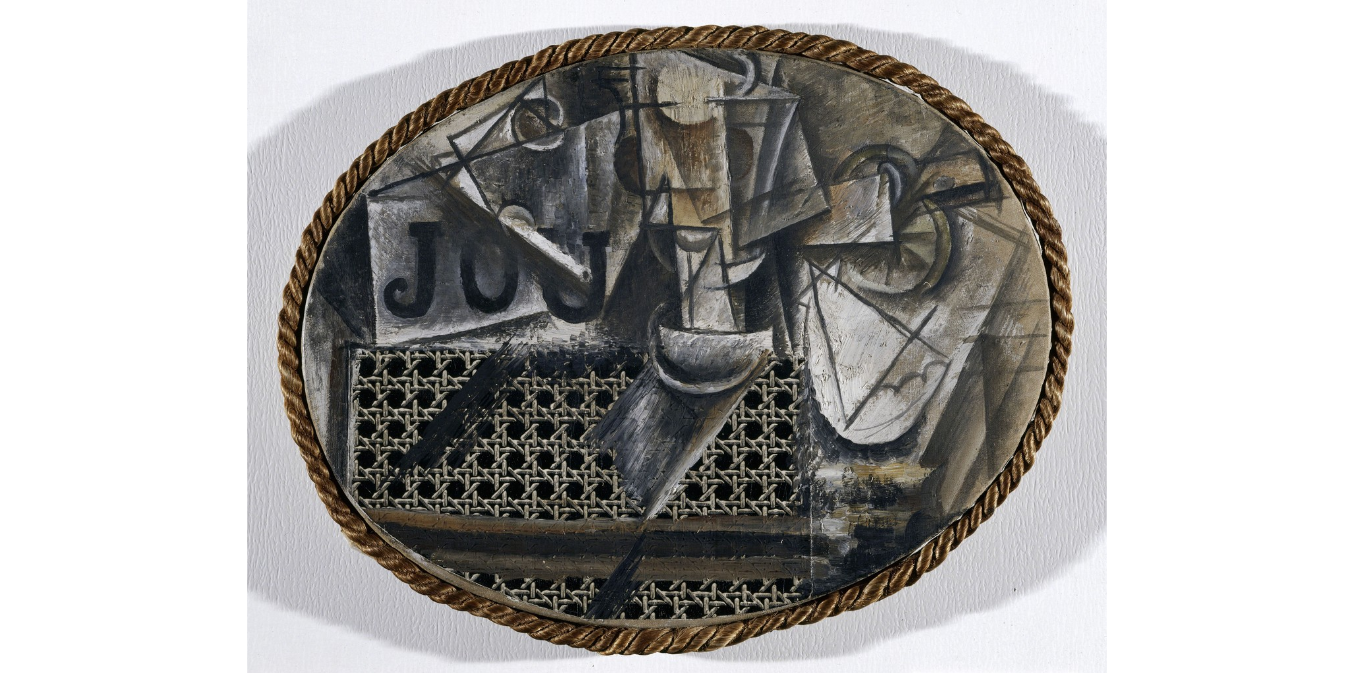
\includegraphics[height=6cm]{graphics/picasso_chair.png}
  \caption{Pablo Picasso, Still Life with Chair Caning, 1912, oil on oil-cloth over canvas edged with rope, 29 x 37 cm (Musée Picasso)}
  \label{fig:Picasso_Chair}
\end{figure}

Moreover, Braque and Picasso questioned the elitism of the art world, which had always dictated the separation of common, everyday experience from the  contemplative realm of artistic creation. Of equal importance, their work highlighted and separated the role of technical skill from art-making. Braque and Picasso introduced a “fake” element on purpose, not to mislead or fool their audience, but rather to force a discussion of art and craft, of unique and mass-produced objects. They ask: “Can this object still be art if I don’t actually render its forms myself, if the quality of the art is no longer directly tied to my technical skills or level of craftsmanship?"

% http://www.nybooks.com/articles/2010/12/09/artist-everything/
% http://www.artchive.com/artchive/S/schwitters.html
After Picasso and Baraque, many artists applied collage and assamblage techniques to their works. Dada artist Kurt Schwitters is one of the productive artists amoung them. In 1918 created his own form of Dada in Hanover called 'Merz', using rubbish materials such as labels, bus tickets and bits of broken wood in his collages and constructions. The nonsense word 'Merz' is generated from the name of the name of a bank: the Kommerz und Privatbank. Merz was soon to become a kind of brand name for almost all his activities and indeed, from 1922, he even began to refer to himself as Kurt Merz Schwitters or simply Merz.

\begin{quote}
The language of Merz now finds common acceptance and today there is scarcely an artist working with materials other than paint who does not refer to Schwitters in some way. In his bold and wide-ranging experiments he can be seen as the grandfather of Pop Art, Happenings, Concept Art, Fluxus, multimedia art and post-modernism...

Schwitters’ work inspired such post-war pioneers as Jasper Johns, Robert Rauschenberg and Joseph Beuys, and he is now seen as the grandfather of post-1945 art movements, from Pop Art to Fluxus, Conceptual Art to site-specific art, and the forerunner of present day artists such as Thomas Hirschhorn, Gregor Schneider and Rachel Whiteread. \citep{webster2011kurt}
\end{quote}

In 1937 after Merzbau had been included in the Degenerate Art Exhibition he fled from Germany to Norway. There he created a second Merzbau. In 1940 he found refuge in England where he started a third Merzbau at Ambleside in the Lake District. The first Merzbau was destroyed in the Second World War, the second by fire in 1951 and the third was left unfinished at his death in 1947. It is now preserved in the Hatton Gallery of the University of Newcastle upon Tyne.

% Yaptığı işte ısrarcı ve üretken. Sürekli inşa ettiği yapılar merzbaular aslında bitmiş bir izlenimi vermiyor. sürekli büyüyor değişiyor. sabit ve bitmiş bir yapısı bulunmamakta.

% FROM The Ruin and the Ruined in the Work of Kurt Schwitters by Gemma Carroll
\begin{quote}
The German avant-garde was working from ruins literally and metaphorically, and trash was both practically and freely available; to use it was an action that took the ruins of our society, its discarded, to question how meaning is constructed. Schwitters is able to use the ruined, the waste products, as an anthropological exploration of society from both its unpleasant outcomes and its decay. \ldots trash was both practically and freely available; to use it was an action that took the ruins of our society, its discarded, to question how meaning is constructed. As he wrote: ‘It grows more or less according to the principle of a metropolis.’ The Merzbau was itself a city; and just as Marx wrote that it was not the materiality of the object but the social relations that create value, the use of urban detritus in particular, the squalid results of mass-produced human relations, infuses the materiality of Schwitters’ work with an anthropological quality. Material has transformed into information, and ‘how’ has surpassed ‘what’ we see. The grottos in the Merzbau that still reveal this detritus most clearly could not be re-created in Bissegger’s reconstruction because, arguably, they are an exploration of absence, an exploration of ruin. \citep{carroll2011ruin}
\end{quote}

% Book: Recycled, Re-Seen: Folk Art from the Global Scrap Heap
Jacknis claims that \quotes{like collage in art or quotation in literature, the recycled object carries a kind of "memory" of its prior existence. Recycling always implies a stance toward time --- between the past and the present --- and often a perspective on cultures --- one's own and others} \citep[as cited in][]{cerny1996recycled}

Recycled object contains within it a reference to two or more distinct times. Whatever their ultimate design or destination, these recycled artifacts are, by definition, "impure", "inauthentic" products of past and present, here and there, "us" and "them". 
%\todo{ref}

% Book: Recycled, Re-Seen: Folk Art from the Global Scrap Heap 
It is claimed that the end result is a category of hybrid objects that bear the mark of at least two distinct domains, each with its won material, meaning, makers, and users \citep{cerny1996recycled} Whatever their ultimate function, each of these objects contains within itself a visual, material, and conceptual reference to multiple technologies, histories and temporalities.

Collages and assemblages can be composed of all types of objects such as trash and found object. The notion of found object is researched by many scholars 
%\todo{ref.}
, but usage in the art has gained new dimensions with the Duchamp's concept of readymade. Industrially manufactured or anything found  anymore can found a place in the art. The most famous example is Fountain (1917) (discussed in the previous chapter), a standard urinal purchased from a hardware store and displayed on a pedestal, resting on its side. Before that first one is Bicycle Wheel. He mounted the bicycle wheel upside down onto a stool. 
% http://www.moma.org/learn/moma_learning/marcel-duchamp-bicycle-wheel-new-york-1951-third-version-after-lost-original-of-1913
When Bicycle Wheel was first displayed, Duchamp encouraged viewers to spin the wheel. Although he claimed to select objects for his readymades without regard to beauty, he said, “To see that wheel turning was very soothing, very comforting\ldots I enjoyed looking at it, just as I enjoy looking at the flames dancing in a fireplace.”

\begin{figure}[h!]
  \centering
  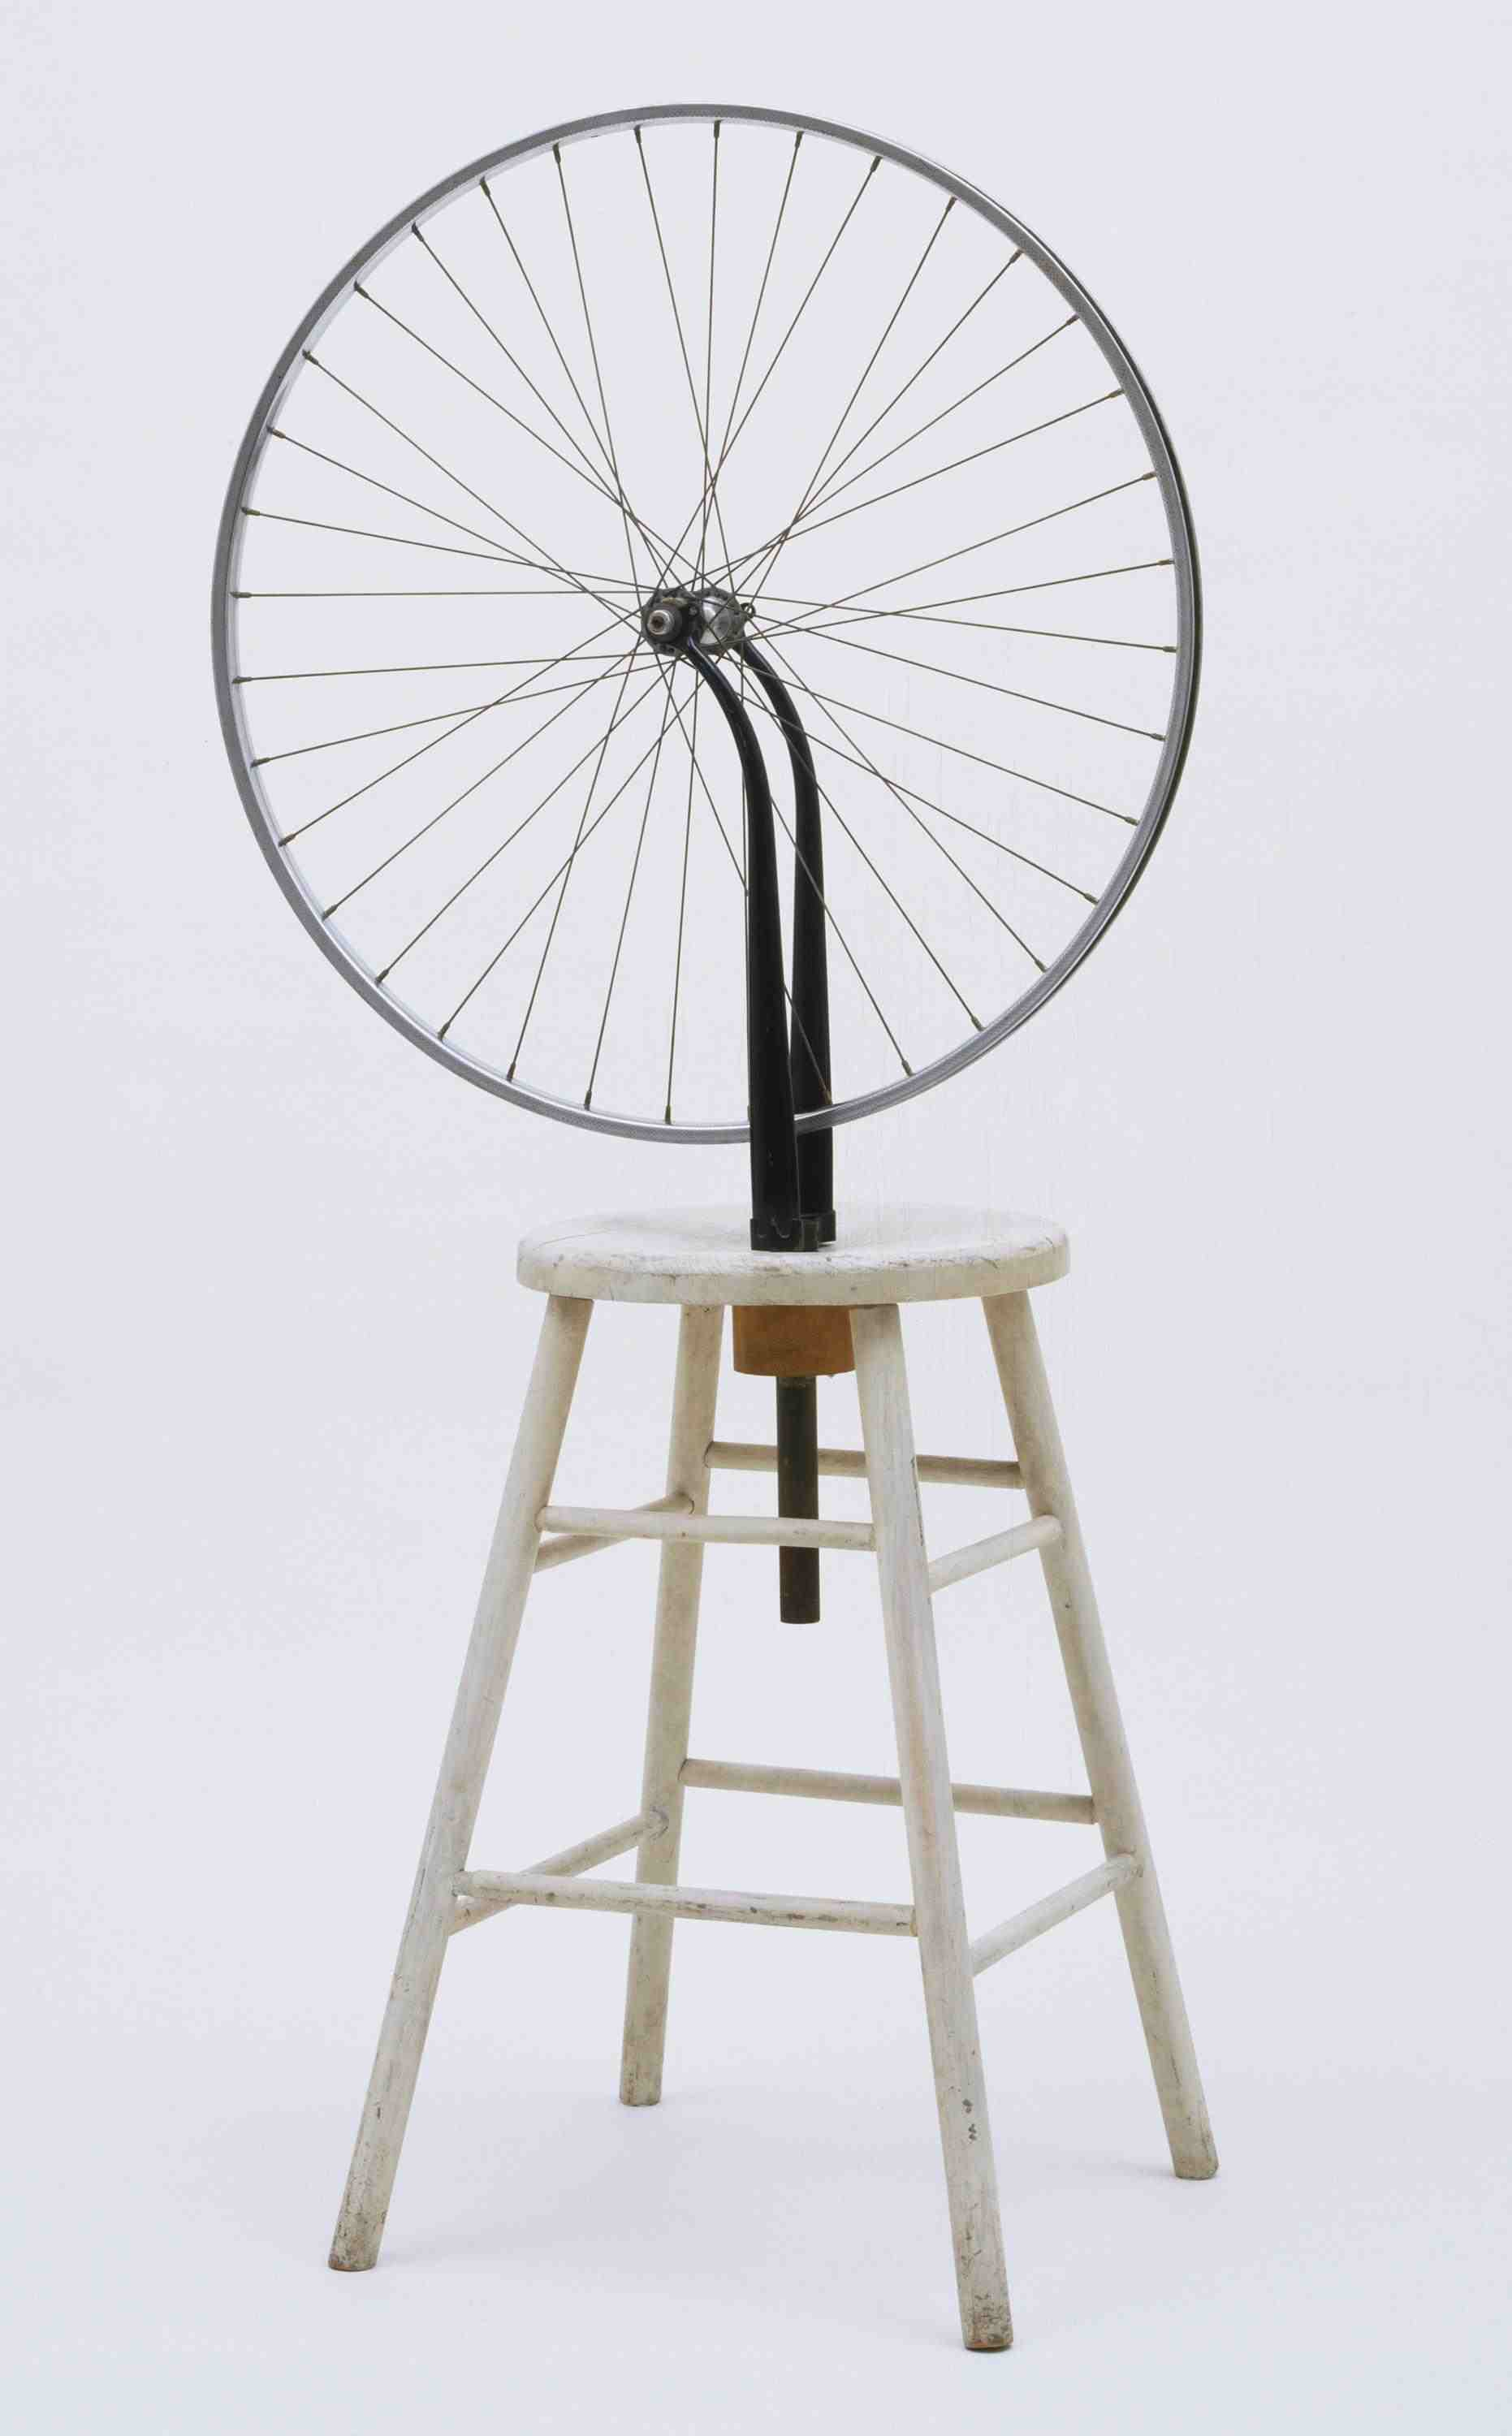
\includegraphics[height=6cm]{graphics/duchamp-bicycle-wheel-1913.jpg}
  \caption{Marcel Duchamp, Bicycle Wheel, 1913 (authorised reproduction 1951, original lost)}
  \label{fig:Duchamp_BicycleWheel}
\end{figure}





% TODO Bunu sadece referans olarak kullanabilirsin, çünkü zaten çok fazla tekrar var.
%\paraphrase{The use of trash as a fine art medium dates back at least to the work of early-20th-century artists such as Fortunato Depero and Kurt Schwitters. Use of found materials, including garbage, has been associated with assemblage art since the 1950s and has been practiced by other well-known artists, including graphic artist Christian Boltanski, sculptor Louise Bourgeois, and photographer Andres Serrano. Art made from garbage has since become much more common in fine arts venues such as museums, galleries, and high-profile installations, including H. A. Schuldt’s famous “Trash People,” which has traveled around the world since 1996 \cite{tauxe2012encyclopedia}.}

% TODO rubbish theoryinin başına konulabilir, referans olarak kullanılabilir.
% Book: Recycled, Re-Seen: Folk Art from the Global Scrap Heap
%\comment{Different meanings for everybody.} 
%\paraphrase{It is stated that same object can have one meaning for one community or culture and another meaning or series of meaning for another. Different objects have different life spans --- different degrees of permanence or disposability --- and that these life spans are socially constituted is also an integrated part of the story \ldots geographic and socioeconomic boundaries of class, caste and culture throughout the world. It is story of people --- the women, men, children etc. one person's trash into another's treasure.}

% TODO MOVE TO COMMON APPROACH
%\comment{Semiotic Context, juxtapositions} \paraphrase{"In popular writing (such as novels), in television, films, music, and other forms of mass expression, the term trash is used to signify work that is of especially low value." \cite{lukas2012garbage}}




%
%
%\summary{Found Object} 
Found object originates from the French \textit{objet trouvé}, describing art created from undisguised, but often modified, objects or products that are not normally considered art, often because they already have a non-art function.

% TODO will not be used. just for rerefence
% Book: Recycled, Re-Seen: Folk Art from the Global Scrap Heap
%\comment{GIFT FROM GOD, NOT KNOWING PREVIOUS STATE} They also states that the practice of tribal people artfully transform Coca-Cola bottle (given as example by the authors). From western trash to tribal treasure. \paraphrase{For the Kalahari Bushmen, the process appears to be one not so much of reusing but of creating anew; not so much transforming, a inventing (p.9).} It stated these found objects is accepted as a gift from gods. A disposable item becomes imminent desire and profound social consequence. (Intercultural recycling.) \paraphrase{Both presentations tell a story about an aesthetic and cross-cultural process --- as well as an economic and political one --- which is defined by the act of recovering and transforming the detritus of the industrial age into handmade objects of renewed meaning, utility, devotion, and sometimes arresting beauty (p.10).}

% TODO will not be used. just for reference
% Book: Recycled, Re-Seen: Folk Art from the Global Scrap Heap
%[Having different meanings] For the same people are not used the items that are scavenged by people who have little or no contact with those who first possessed them, and may neither know nor care about their originally intended function. It is case from the film and also the case depicted in the real life photographs taken by anthropologist michael leahy which document his first colonial contact with new guinean highlanders.

% TODO will not be used. just for reference
% Book: Recycled, Re-Seen: Folk Art from the Global Scrap Heap
%\todo{yerlinin fotoğrafı}
%\quotes{Renowned early-twentieth century anthropologist Michael Leahy encountered a Wabag man from Papua New Guinea wearing an aluminum whole wheat biscuit tin on his head. In the symbol system of this culture, large, bright, and shiny ornaments are connote health, well-being, sexual attractiveness, and the approval of the ancestors.} \todo{ref.}





%(Summary From Paul M Camic.) 
%The term found object, as used in this article, refers to an existing object or artifact that is picked up (found) and generally not bought or originally intended as art, yet it is also considered to have some value (e.g., aesthetic, novelty, remembrance) to the finder. It is during the locating and finding process that the value of the object, once considered to be junk or rubbish, changes. The junk object becomes transformed into the valued found object. Objet trouve, translated from the French as “object found,” appears to have been first used by Marcel Duchamp in 1913 in reference to objects he made use of in his “readymade” art (Richter, 1965). His earliest known application for an objet trouve was seen in his well-known piece Bicycle Wheel, “where he had simply upturned a wheel on a stool” (Gale, 1997, p. 97) and labeled it a work of art. A more public and controversial introduction of the readymade occurred in 1917 when Duchamp attempted but failed to exhibit the highly contentious piece The Fountain, where a single white urinal became a readymade piece of art (Tomkins, 1996). These pieces were the beginning of Duchamp’s shift from an art striving for beauty and possessing a higher complex or hidden meaning beyond what was seen to an art form that made use of, and occasionally celebrated, the common materials and objects found in everyday living.

Gascoygne (1936), writing about the artist’s use of “the strange medley of materials” (p. 169), referred to as objets trouve in Surrealist art, suggesting that the artist “discovers a hidden symbolic significance in the [found] object which is preserved when the object is ‘framed’ as art” (p. 170). The finder discovers an unrealised significance in the object. A new boundary is formed around the object by the finder through removing it from its found environment and placing it in a new one, thus empowering the finder in the role of creating a new reality for the object. He argued that the found object, before it is found, approximates a zero value aesthetically; the zero value increases for the finder---beholder on discovery of the object and increases further if the object is placed in another context. \ldots the meaning of material objects was derived from their symbolic relation to another (e.g., person, time, place, experience) rather than through their physical attributes (Causey, 2003; Csikszentmihalyi \& Rochberg-Halton, 1981). 
%\todo{parap. ref.}


%How a region of flexibility develops, what social factors are involved in taking innovative and creative responses toward rubbish, and how an individual changes (and enhances) his or her creative responses toward society’s detritus are areas that require additional examination. (Important points a gap in the literature. Although Parsons article analyze practices, it is not very broad and detailed. Further what is the importance of it is missing.)

%The importance and enjoyment of found objects to those who participated in this study, using them in various ways and for different reasons, were strongly evident. The interaction between finder and object is an attempt to make meaning of an object that has been found, and by being found and desired becomes transformed.

%Gascoygne (1936) recognized that finding an unrealized significance in a material (found) object was empowering partially because, through the creative agency of the finder, the object’s aesthetic value had increased from zero to something greater. The transformation of rubbish from a negative value to a positive value requires the finder to develop a symbolic meaning, and sometimes a functional use, for the object that goes beyond its present situation as culturally labeled detritus while simultaneously responding to its current physical and aesthetic elements. When the found object is seen by the finder as a symbol representing another entity (e.g., when an old blue bottle with foreign lettering comes to symbolize far away intrigue, mystery, and sophistication), support is given to what Dittmar (1992) described as socially constructing a material identity for the object. Expanding on Dittmar’s use of a social interactionist perspective, the results of the present study support the possibility that the entire found object process---finding, reclassifying, and reusing objects---becomes a symbol of identity for the finder. This supports Digby’s (2006) argument that individuals make use of salvaged objects as souvenirs, which are no longer part of the commodity cycle, to rework and construct individual and social identities.

%An important difference, however, which also appears to contribute to the aesthetic experience, takes place when discovering an object unexpectedly in a nonpredetermined place and time. Unlike appreciating art in a museum, which is a boundaried activity occurring at a scheduled time and place with the anticipation of finding and looking at art objects, finding discarded objects can occur anywhere at anytime and thus, according to participants, can “trigger” a burst of sensory attention and a “surge” of cognitive activity on the part of the finder. 

%Results of this study also support consideration of found objects as important artifacts that are signifier of cultural meaning.

% [TODO adapt for my case] Found objects first came to the attention of the general public through their use by artists in early part of the 20th century. To help contextualize the application of found objects, the following section provides an overview of their use by Western artists. This is followed by an examination of objects in human development and includes aspects of psychoanalytic theory, material objects and their relationship to identity, selected cognitive theories, and an outline of the social life of objects through rubbish theory.





%
%
\section{Examples from contemporary artists}
In the light of discussions at previous section, some of the main strategies and approaches of artist are analyzed. First one is related with found objects. In this section focus will be shifted to the examples from contemporary artists.

% Neden bu işler, neden bu sıra?

% Neden çöpü kullanıyorlar. Bunu belirmek gerekli. İlki sanata farklı bir obje sokarak saflığını bozma, hazır yapım ile geleneksel yöntemlere karşı çıkış, fikrin ön plana çıkması. Visual uniqueness, aesthetics dimension, Economic reasons

Photobooths are machines that place crowded places and with affordable cost people can get their photos. It is a pheonema that attract attention of artist and researchers such as Martin Parr and Gerry Badger who published history of them as two volume.

In the French film Amélie\footnote{Original title: Le fabuleux destin d'Amélie Poulain, in english: The Fabulous Destiny of Amélie Poulain} directed by Jean-Pierre Jeunet in 2001, young male character collects photos that are torn up and thrown away by their owner near photo booths spread through train and metro stations of Paris. He collects them and glue them together in a photo album. In the film photo booths and found photos are centrally catalytic. Amélie falls in love with him when she realize him searching for found photos. After his photo album passed to Amélie, she looks every page of photo album again and again. Through the images of unknown people, she establishes narratives that point out the significance of these images even if they are thrown away. The important part of the film, images of a man are generated who scanvage the photos of another people. There are a lot of artist who collects discarded items but their process is not well documented. Therefore we are not aware of the artistic process. 

\begin{figure}[h!]
  \centering
  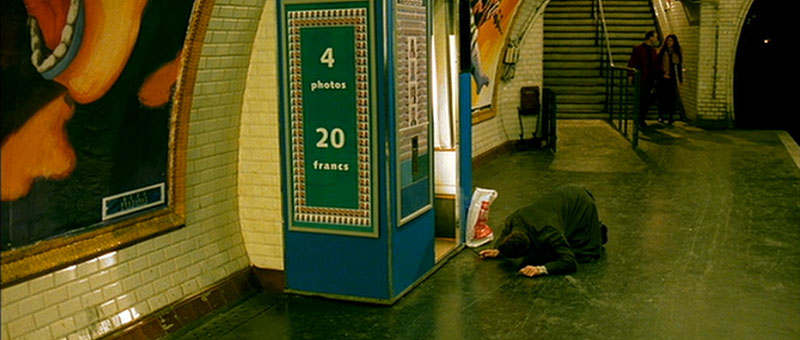
\includegraphics[height=6cm]{graphics/amelie_01.jpg}
  \caption{Still image from Amélie}
  \label{fig:Amelie}
\end{figure}

Prior to film Amélie, British artist Dick Jewell published a book in title of "Found Photos" in 1977. It is a collection of photobooth images that had been thrown away or torn up by the people in the photos. \cite{walker2010dick} comments on that it is "always a joy to look through." Images capture diverse range of activities and expressions of people using photo booth machine. They are scavenged by the artist from the photo booths of London. The reasons of why photos are rejected vary including technical problems like flash or posing time. On the other hand, some of them are very good condition, and it is a mystery that why they are rejected. Walker explains that the 

\begin{quote}
gap between our exterior perception of the image and what must have been the internal dissatisfaction of the original subject results in some of the effective moments in Found Photos, where the images are not only bizarre and wonderfully funny (as many of them are) but also profoundly moving.
\end{quote}

Walker argues that even if photo booths are mechanic and simple application of photography while capturing everyday life, leave behind such ambiguous and mysteries that some people trace them. "Dick Jewell’s approach with Found Photos was less interventionist, presenting the images themselves in the spirit of either an anthropologist showing his finds or a conceptual artist claiming bits of the real world as ‘readymades’." His mode of discovery includes climbing to look at the top of the box and looking for the nearest waste bin. Badger describes Found Photos as ‘both a conceptual artwork and a sociological footnote’.

\begin{figure}[h!]
  \centering
  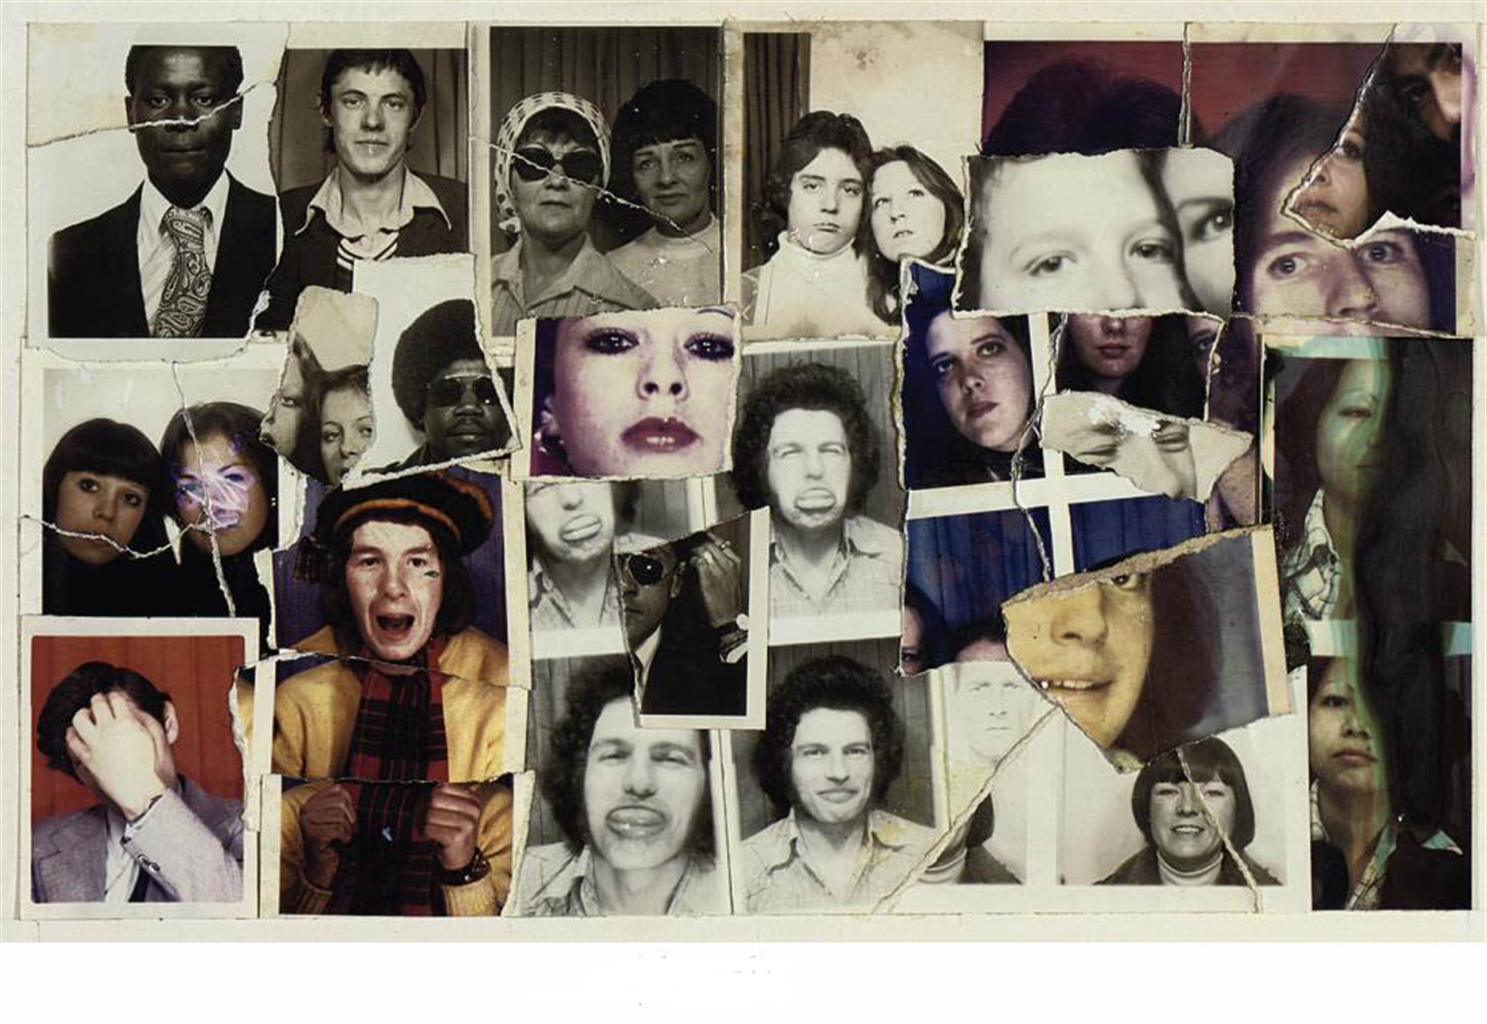
\includegraphics[height=6cm]{graphics/DickJewell_FoundPhotos.jpg}
  \caption{Dick Jewell, Found Photos, 1978}
  \label{fig:DickJewell_FoundPhotos}
\end{figure}

On the other side for another artist photographs serve a function to record his daily trash. Tim Gaudreau photographed every object that he threw away for one year. At the end around five thousand images are covered all the gallery and opened to visitors. He notes that it just started as a documentation of his discards, but later it became (part of his life and) an obsession that he can not able to easily quit off. He says that "this collection of images intimately displays what I do, what I consume. It reveals me." Like in the case of Tracey Emin trash turns to a medium that is used to express oneself. People are not only composed of the listed items in the CVs like in the film Fight Club Tyler Durden draws attention to the narrator by saying: "You are not your bank account". It is an effective way of looking things left behind rather that things put forward. Through this project, artist reached better understanding what he is and notes that this project changed his consumption choices and patterns.

\begin{figure}[h!]
  \centering
  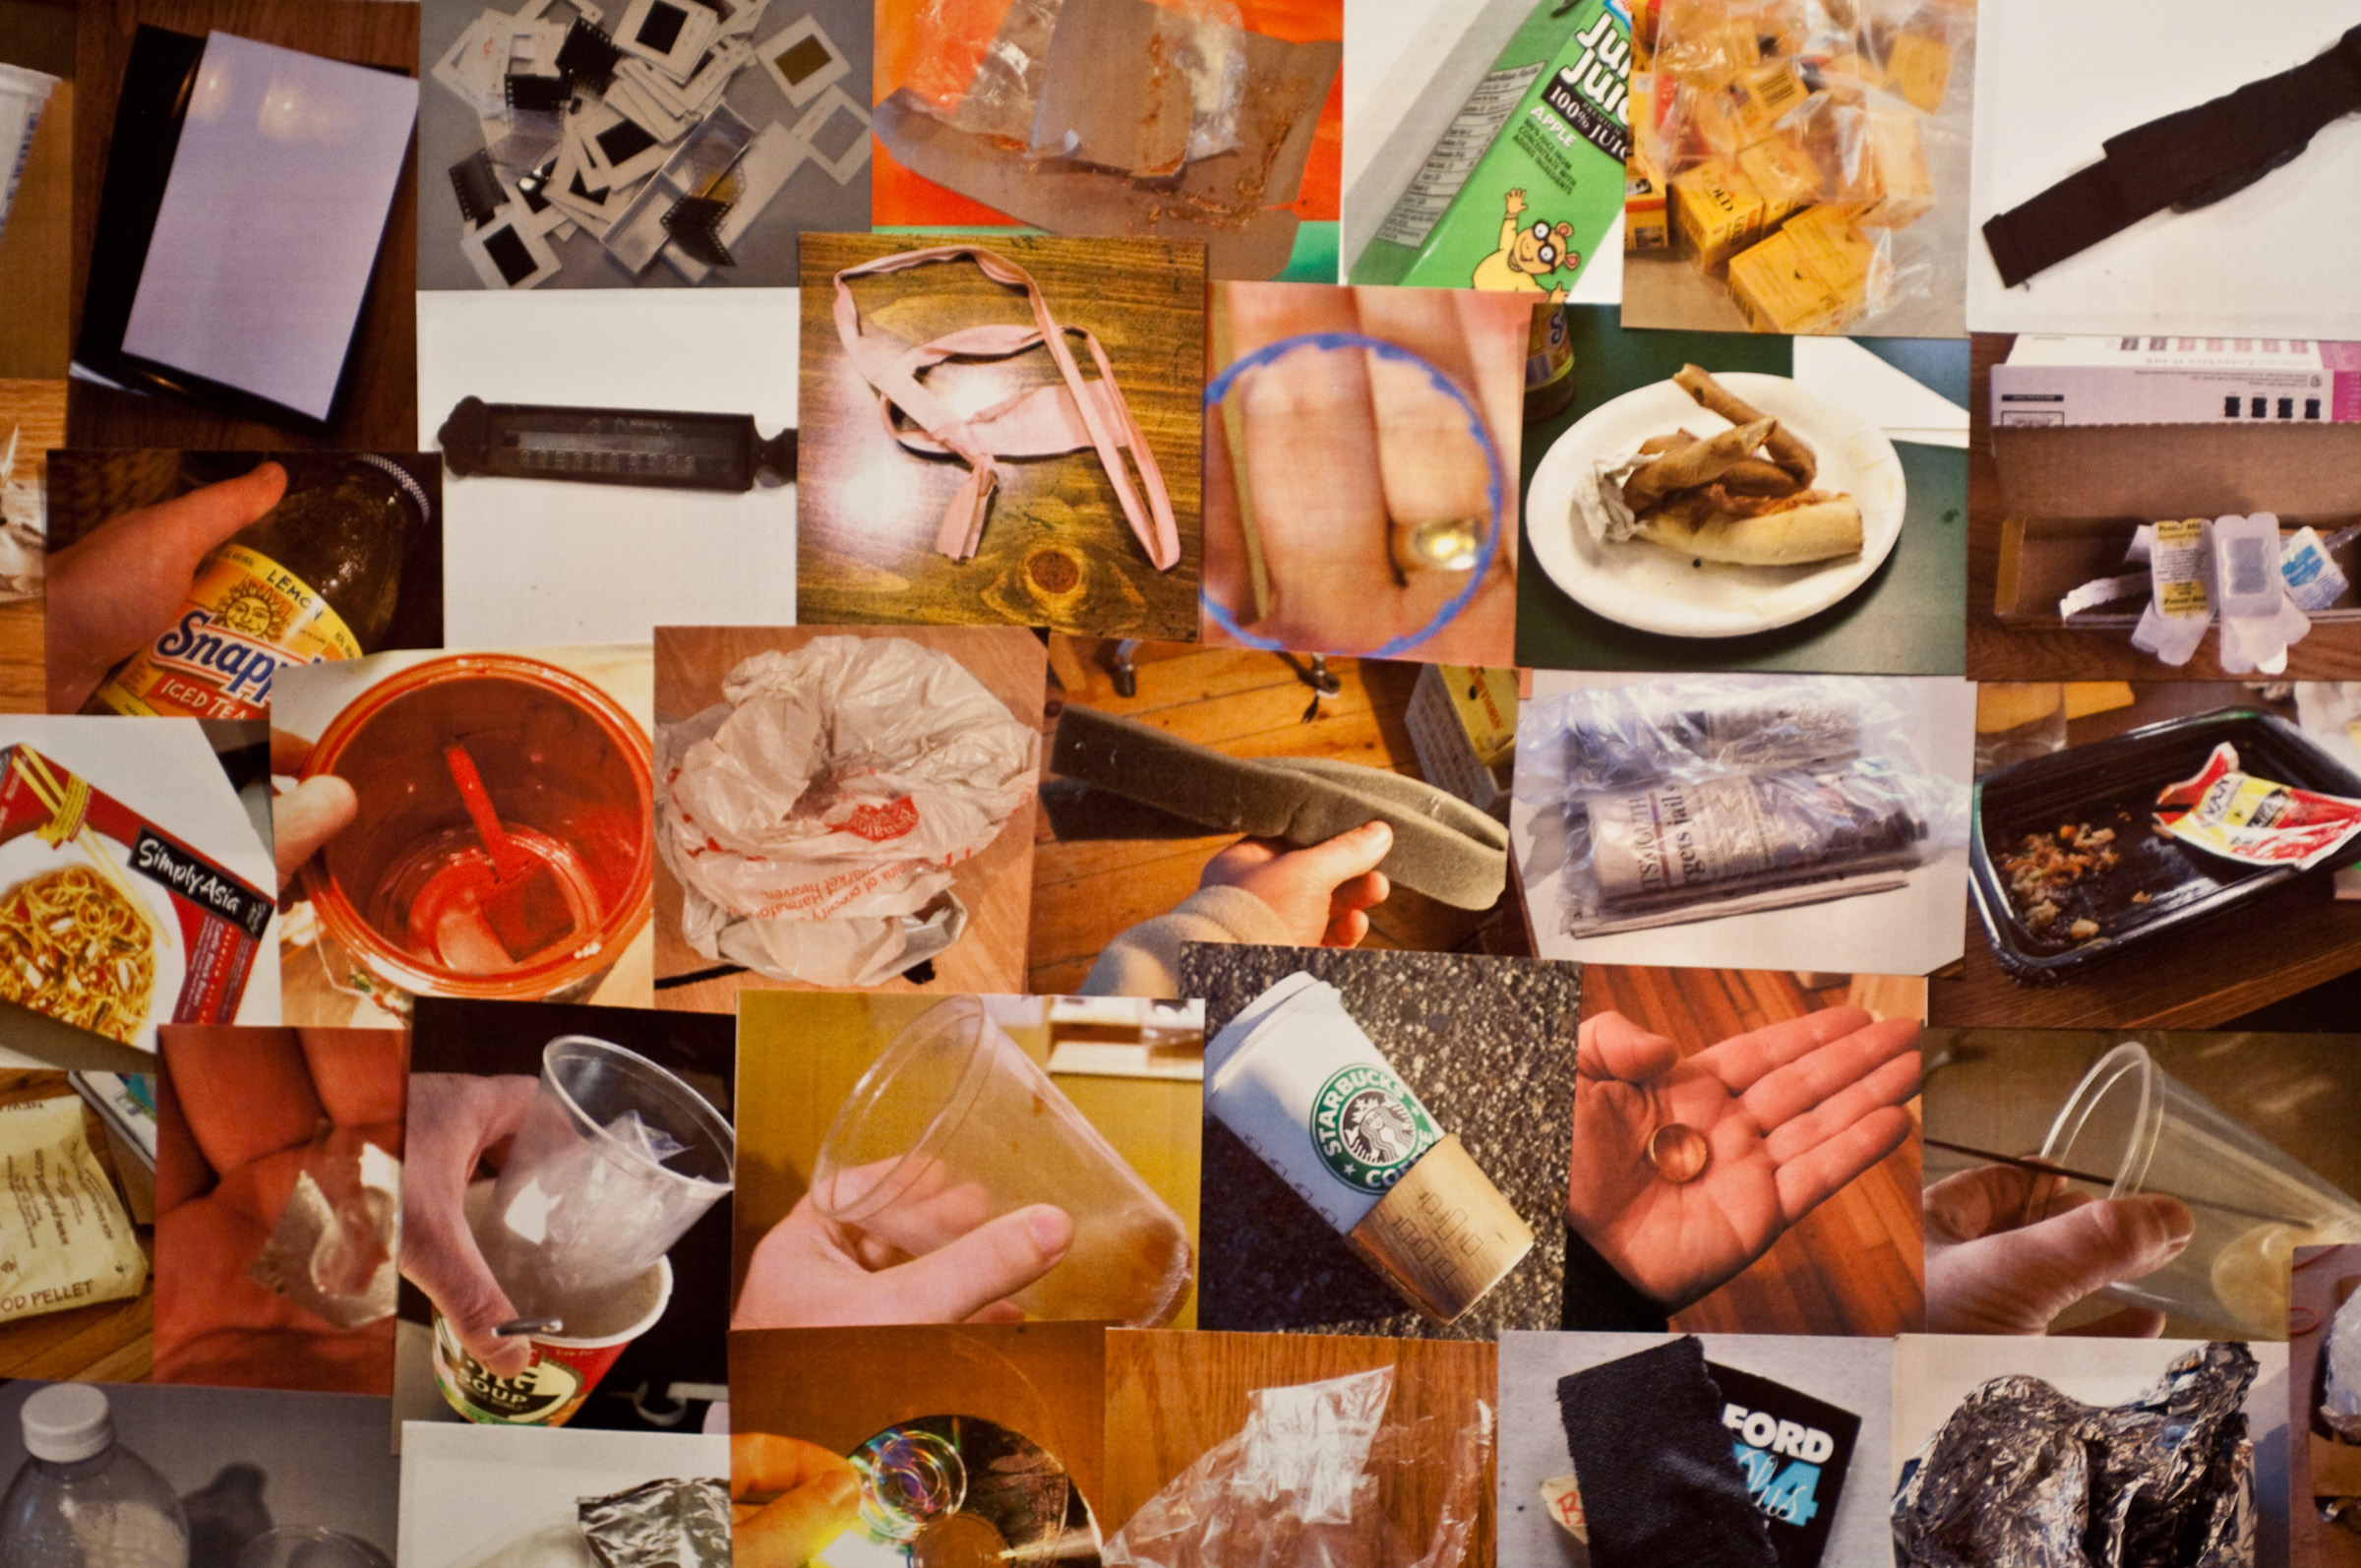
\includegraphics[height=6cm]{graphics/TimGaudreau_SelfPotraitRevealedByTrash.jpg}
  \caption{Tim Gaudreau, Self-Portrait as Revealed by Trash: 365 days of photographing everything I threw out – Variation I, 2006}
  \label{fig:TimGaudreau_SelfPotraitRevealedByTrash}
\end{figure}

Filomena Cruz turns her lens to the city and its trashes that are left behind, thrown away and squeezed on the sidewalk or pavement. In her photographic series "Road Kill", she captures tiny "trash corpses" that are generally ignored and out of sight. In other words, the skin of city revealed through her photos in micro scale. On the skin of city there are lots of trash including "a piece of chewing gum with an "engraved" leaf; a flattened-out tube; a corroding paper napkin with a still intact heart; or a frog-green Crayola melting in the heat, all speak the language of "worthlessness" suddenly becoming meaningful" as looked through the window of they capture the city life and skin of the city that we touched. She shows us tiny details of huge cities. (Somehow these trashes for all effort succeeded to stay in the towns.) These trashes can not be removed from the city but moved ones are stacked on landfill, and they are not tiny as they are.

\begin{figure}[h!]
  \centering
  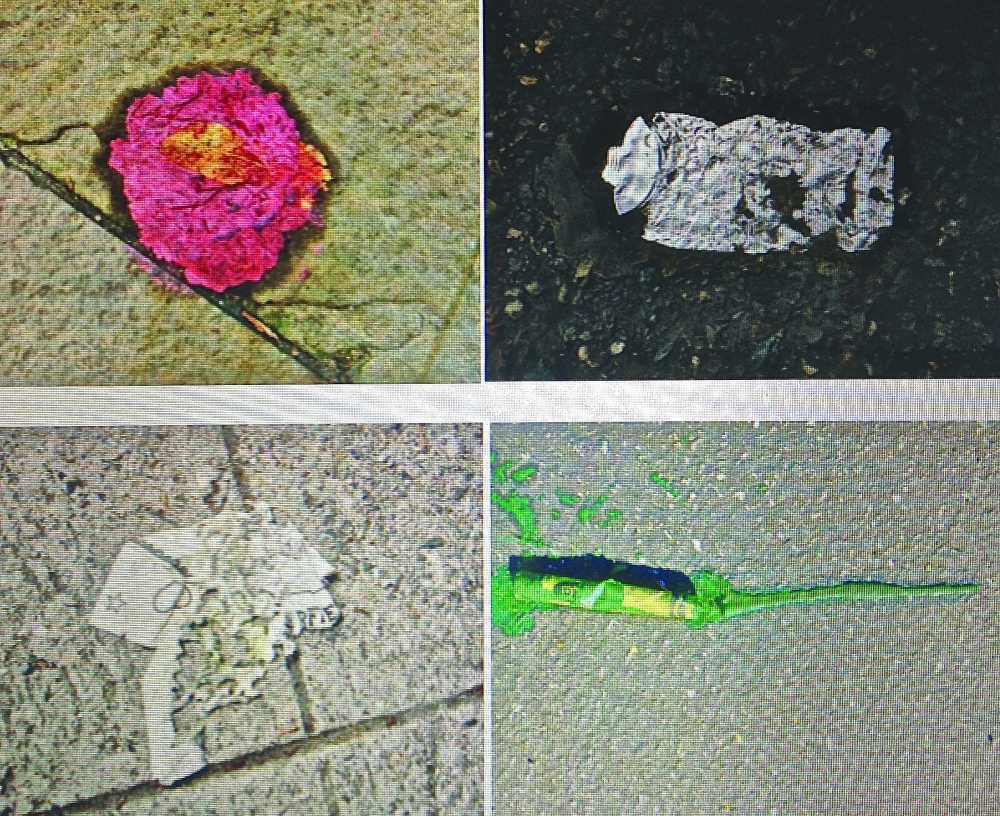
\includegraphics[height=6cm]{graphics/FilomenaCruz_RoadKill_ReVista.jpg}
  \caption{Filomena Cruz, Road Kill, 2014, Photography}
  \label{fig:FilomenaCruz_RoadKill_ReVista}
\end{figure}

In the documentary film, Waste Land, Vik Muniz frames portraits of \textit{catadores} who are pickers of recyclable materials on the dump. He visits them at one of the biggest open-air garbage dump outside of the Rio de Janeiro home of the millons of people. Film documents whole process of development and production of "Pictures of Garbage" made of collected trash from dump. He selects unusual materials and people for potraits rather than the powerful and notable people as commonly encountered at Renaissance. To create portraits of \textit{catadores} there is any other material than trash because of they are already build up their life in trash of city. [Also these image are sold an auction and earned money donated to the \textit{catadores}. The images of trash moved to beloved places such as homes and museums. As stated in the rubbish theory they transformed to a durable object.]

\begin{figure}[h!]
  \centering
  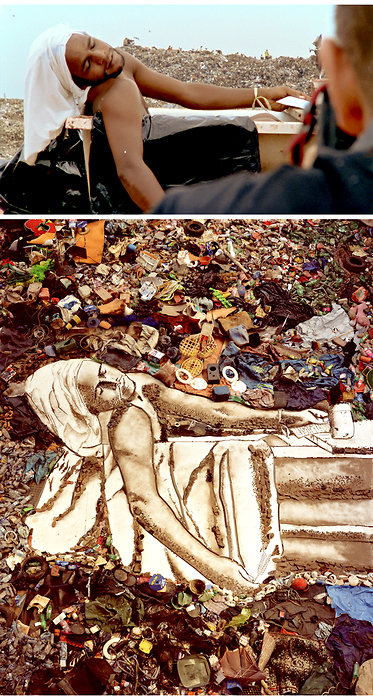
\includegraphics[height=10cm]{graphics/vik-muniz-picturesofgarbage0.jpg}
  \caption{Vic Muniz, Ironing Woman (Isis), 2008, mixed media, }
  \label{fig:VicMuniz_PicturesOfGarbage}
\end{figure}

Not only monumental portraits extracted from the dump but also an orchestra is grounded up from the dump of Paraguay pioneered by Favio Chávez and Nicolás Gómez. Favio Chávez is a music teacher, and Nicolás Gómez is a garbage picker. They live in Cateura at Paraguay. It is a one of the poorest villages where people live among the sea of garbage. "A violin is worth more than a house here," says Favio Chavez in documentary film. The orchestra's director and founder. Favio Chavez director and founder of the orchestra whose instruments such as violins, flutes and cellos are built from collected trash by Nicolás Gómez. Players of the orchestra are compiled from the children who are hopeless for their future. In the midst of such an existence, these musicians have created something both special and truly awe-inspiring. They are given birth to an orchestra that plays the masterpieces of classical music composed by Mozart, Beethoven, and Vivaldi. Trash turned to treasure and totally ironic that a signifiers of high culture like classical music can be even played with imperfect instruments. For them and also, most of the people it is not affordable to buy an instrument and get the education of classical music. What they create is actually not expected from them, and their success is not limited with their location. They have given concerts around the world. 

%"People realize that we shouldn't throw away trash carelessly," says Chavez at the end of the trailer. "Well, we shouldn't throw away people either." \quotes{The world send us garbage. We send back music}.

% Resistance to all hard conditions

\begin{figure}
    \centering
    \begin{subfigure}[b]{0.47\textwidth}
        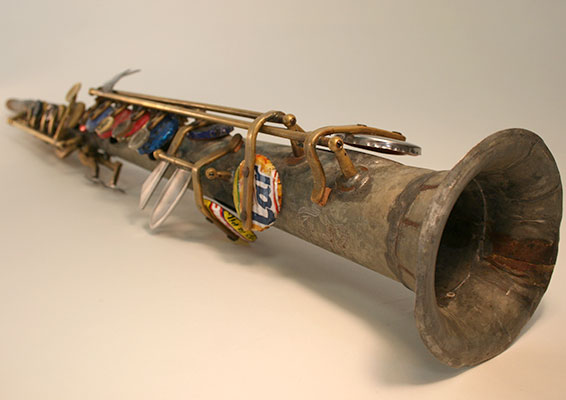
\includegraphics[width=\textwidth]{graphics/landfill_harmonic-sax.jpg}
        \caption{Sax}
        \label{fig:landfill_harmonic-sax}
    \end{subfigure}
    \begin{subfigure}[b]{0.47\textwidth}
        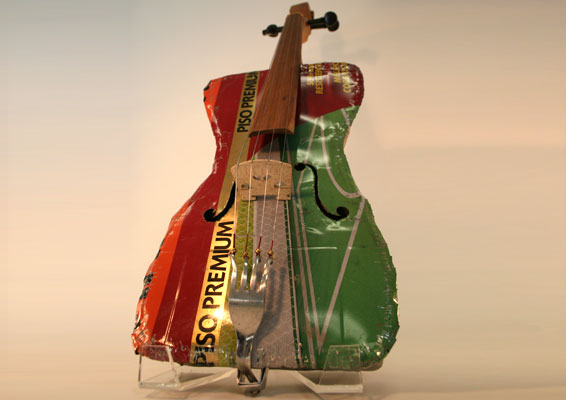
\includegraphics[width=\textwidth]{graphics/landfill_harmonic-violin.jpg}
        \caption{Violin}
        \label{fig:landfill_harmonic-violin}
    \end{subfigure}
    \caption{Instruments of Recycled Orchestra}\label{fig:animals}
\end{figure}

As noted that recycling as an economic strategy of survival in developing countries throughout the world. Creative production that is motivated, primarily, by adverse conditions of economic necessity. Economic survival and adaptation are influential factors for both the makers, who build an informal business on the making and selling of recycled goods and the local consumers, for whom the market for affordable, utilitarian goods is devised. (p25)

They build their musical instruments from what is available around. This project can be seen as a bricolage practice. Dictionary meaning; something constructed using whatever was available at the time. \quotes{Claude Levi-Strauss notes that the \textit{bricoleur} works not from the principle of making things only if natural resources are available but makes things according to those things at hand, making do with what is available. It is an expression that, like the natural cycles of the Earth, attempts to make something new from something old. \citep{levi1966savage}} The \textit{bricoleur} is \ldots someone who works with his [or her] hands and uses devious means compared to those of a craftsman \citep{levi1966savage}.

\quotes{\ldots someone that creates bricolage is described as a bricoleur, an odd-job man who works with his hands, employing the bricoles, the scraps or odds and ends.}

\begin{quote}
[He or she] is adept at performing a large number of diverse tasks; but, unlike the engineer, he [or she] does not subordinate each of them to the availability of raw materials and tools conceived and procured for the purpose of the project. His [or her] universe of instruments is closed and the rules of his [or her] game are always to make do with “whatever is at hand,” that is to say with a set of tools and materials which is always finite and is also heterogeneous because what it contains bears no relation to the current project, or indeed to any particular project, but is the contingent result of all the occasions there have been to renew or enrich the stock or to maintain it with the remains of previous constructions or destructions.\cite{levi1966savage}
\end{quote}

%\begin{quote}
%The bricoleur, says Levi-Strauss, is someone who uses 'the means at hand,' that is, the instruments he finds at his disposition around him, those which are already there, which had not been especially conceived with an eye to the operation for which they are to be used and to which one tries by trial and error to adapt them, not hesitating to change them whenever it appears necessary, or to try several of them at once, even if their form and their origin are heterogenous---and so forth. There is therefore a critique of language in the form of bricolage, and it has even been said that bricolage is critical language itself\ldots If one calls bricolage the necessity of borrowing one's concepts from the text of a heritage which is more or less coherent or ruined, it must be said that every discourse is bricoleur.\cite{derrida1993structure}
%\end{quote}

%\begin{quote}
%The engineer, whom Lévi-Strauss opposes to the bricoleur, should be the one to construct the totality of his language, syntax, and lexicon. In this sense the engineer is a myth. A subject who would supposedly be the absolute origin of his own discourse and would supposedly construct it 'out of nothing,' 'out of whole cloth,' would be the center of the verbe, the verbe itself. The notion of the engineer who had supposedly broken with all forms of bricolage is therefore a theological idea; and since Lévi-Strauss tells us elsewhere that bricolage is mythopoetic, the odds are that the engineer is a myth produced by the bricoleur.\cite{derrida1993structure}
%\end{quote}

% TODO Bunu bitirirken de bir şeyler demek gerekli.

In the scope of painting different than the works in the previous chapter (paintings on tea bags and coffee cups) historical potraits of notable people are painted onto the flattened aluminum drink cans which are disposable objects. The people in the figure X is General Jefferson C. Davis who was an officer at United States Army in 19th-century. Selected persons can be viewed as a member of the higher or ruling class of society. Therefore Kim Alsbrooks, painter of these works, might have thought that to make trash is more valuable, their face will be good. Or vice versa. She probably use trash to criticize social elite of that time. 

\begin{figure}[h!]
  \centering
  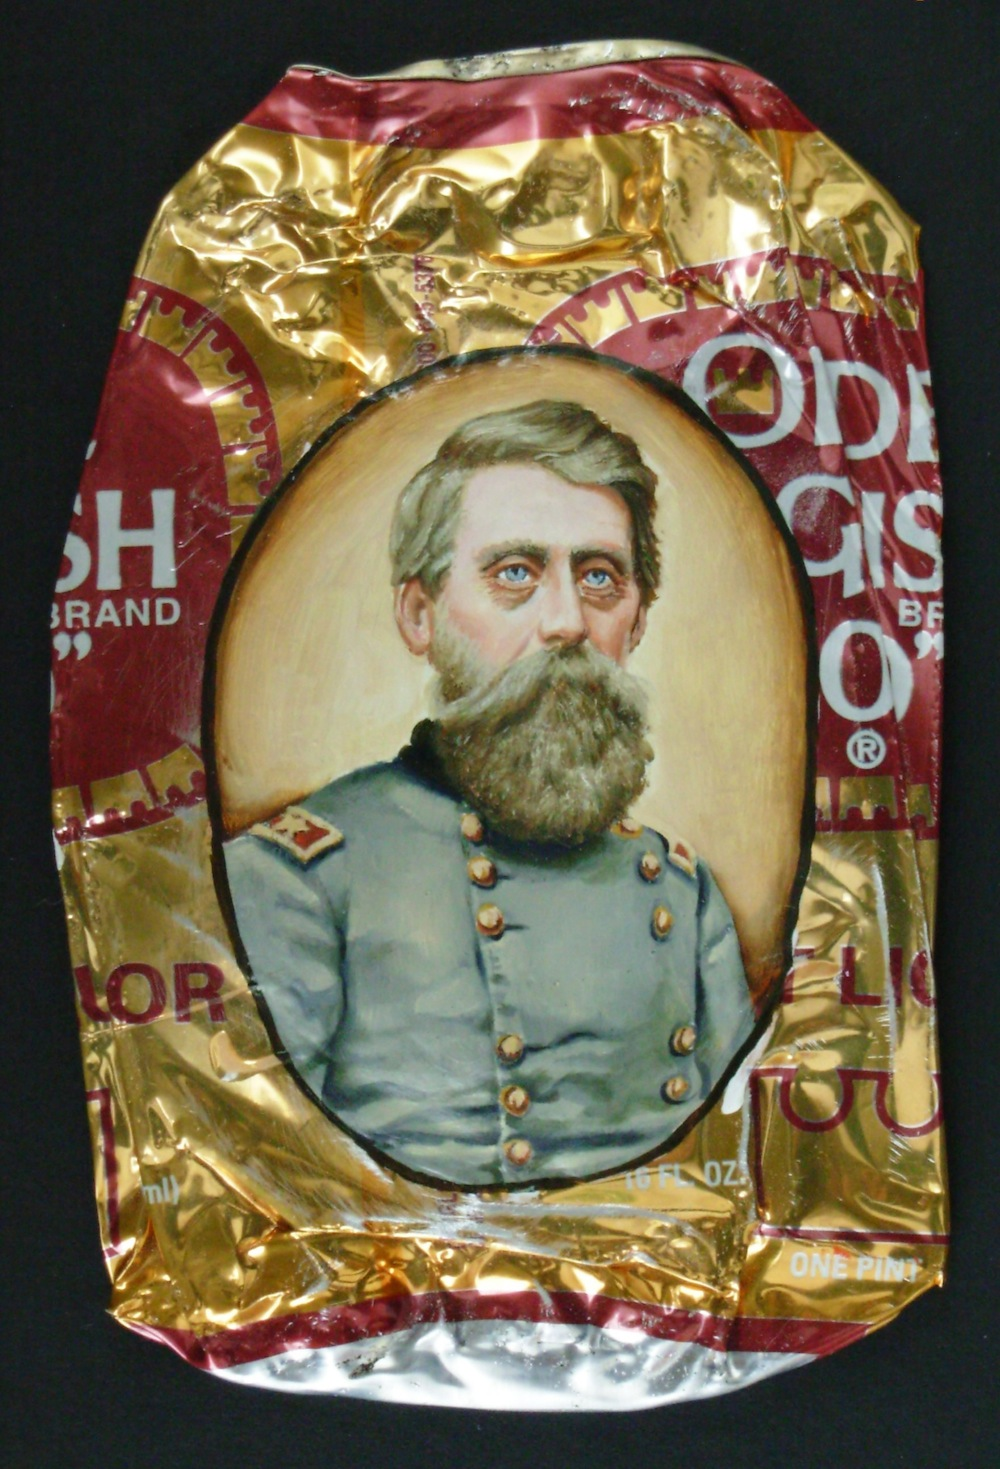
\includegraphics[height=8cm]{graphics/Alsbrooks.jpg}
  \caption{Kim Alsbrooks, Gen. Jefferson Davis, 2015, oil on aluminum can}
  \label{fig:Alsbrooks}
\end{figure}

Not all the time and every artist turn trash into different objects, sometimes they only trash them. Michael Landy's Art Bin is one of them. It is a room size transparent bin placed inside of the art gallery. He invites people to bring their own artworks of failed attempts. Some of the notable contemporary artists such as Damien Hirst, Gillian Wearing, Tracey Emin and Mark Titchner participated in by throwing their sculptures, paintings, and prints into the Art Bin. People publicly toss their work from a high platform, and all of them can be seen outside of the transparent walls. He listens to the story and the failure of the artworks from their creator, and it is not allowed to throw others work. At one side he criticizes the idea of not aware of that artist also have lots of failures. People only can see the final work in the galleries and museums. In this work he break-ups this notion that encouraging the artist reveals their failures to the public. Like his words, it is “a monument to creative failure”. On the other side, there is a provocative approach to the art and art objects by saying that "Nothing is too good for the art bin." There is no limitation of throwing away even if art. 

\begin{figure}[h!]
  \centering
  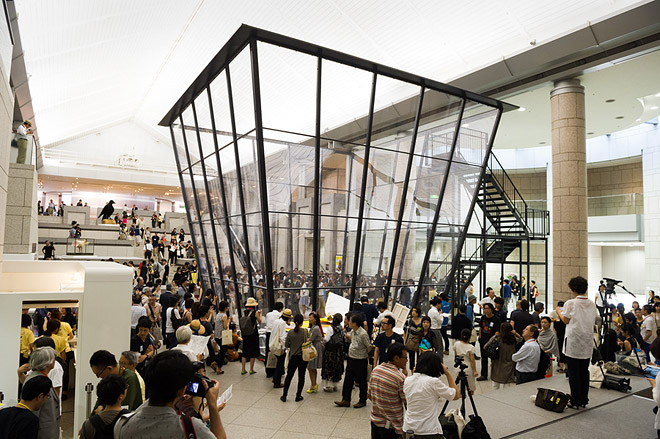
\includegraphics[height=8cm]{graphics/MichaelLandy_ArtBin.jpg}
  \caption{Michael Landy, Art Bin, 2014}
  \label{fig:MichaelLandy_ArtBin}
\end{figure}

% Landy'nin yaptığı bir çok iş aslında çöple ilgili olduğu savunulabilir. Hepsinin anlatmak mümkün olmasada bir diğer için sahip olduğu tüm eşyaları bozmasıyla ilgili. Daha önceden bahsettiğim geri dönüştürme tanımları ile ilgili olarak bu işi downcycling yöntemi arasında görülebilir. 

Not all artist transform trash although some deconstruct them. Michael Landy is one of them. Michael Landy's Break Down Inventory is a two-week show (display) of destruction process of his all possessions on a dissemble line with the help of 10 workers. Firstly they are classified and recorded for three years and the deconstructed in two weeks by separating every element to the smallest part. Reveal all his possessions and deconstruct of them while he is alive. He turns them to rubbish and makes them unusable. Breaking down the all the meaning. Breaking down the connections. It can be an example of a downcycling process. It is preferred to decompose all the complex link and relationships between the objects. They are not just ordinary things they are possessions of the artist. Break Down 2001, in which he systematically destroyed all his personal possessions. His work examines what we value and what we discard, consumerism and waste, and human labor and its worth. It happens in public space. People can see the process. This process lasts two weeks at a place where people buy goods.

\begin{figure}[h!]
  \centering
  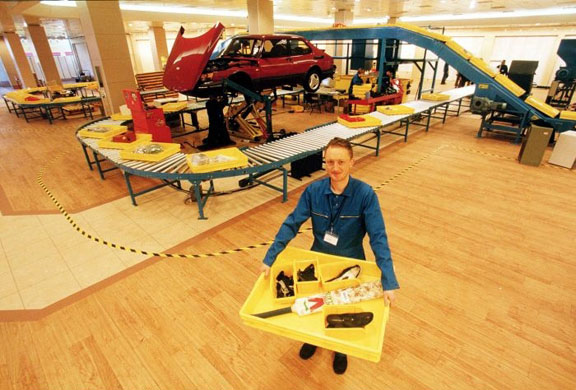
\includegraphics[height=7cm]{graphics/MichaelLandy_BreakDown.jpg}
  \caption{Michael Landy, Break Down, 2001}
  \label{fig:MichaelLandy_BreakDown}
\end{figure}

% http://www.publicbooks.org/interviews/recycling-literary-culture-a-conversation-with-lucia-rosa, http://www.eloisacartonera.com.ar/ENGversion.html
%\textbf{Eloísa Cartonera.} a work cooperative in Buenos Aires, proudly produces handmade books with cardboard covers. \quotes{We purchase [\ldots] cardboard from the urban pickers (cartoneros) who pick it from the streets. Our books are on Latin American literature, the most beautiful we had a chance to read in our lives.} \quotes{Some of them are preserved as art books at university libraries, while others circulate as literary pieces expected to disintegrate in time---something anticipated of the material they are made from.} [from PAOLA IBARRA, ReVista]

%It reminds me that litreary is also a combination of reused thing. Because to create meanings we reuse words and idioms again and again with different combination.

%\begin{figure}[ht]
%  \centering
%  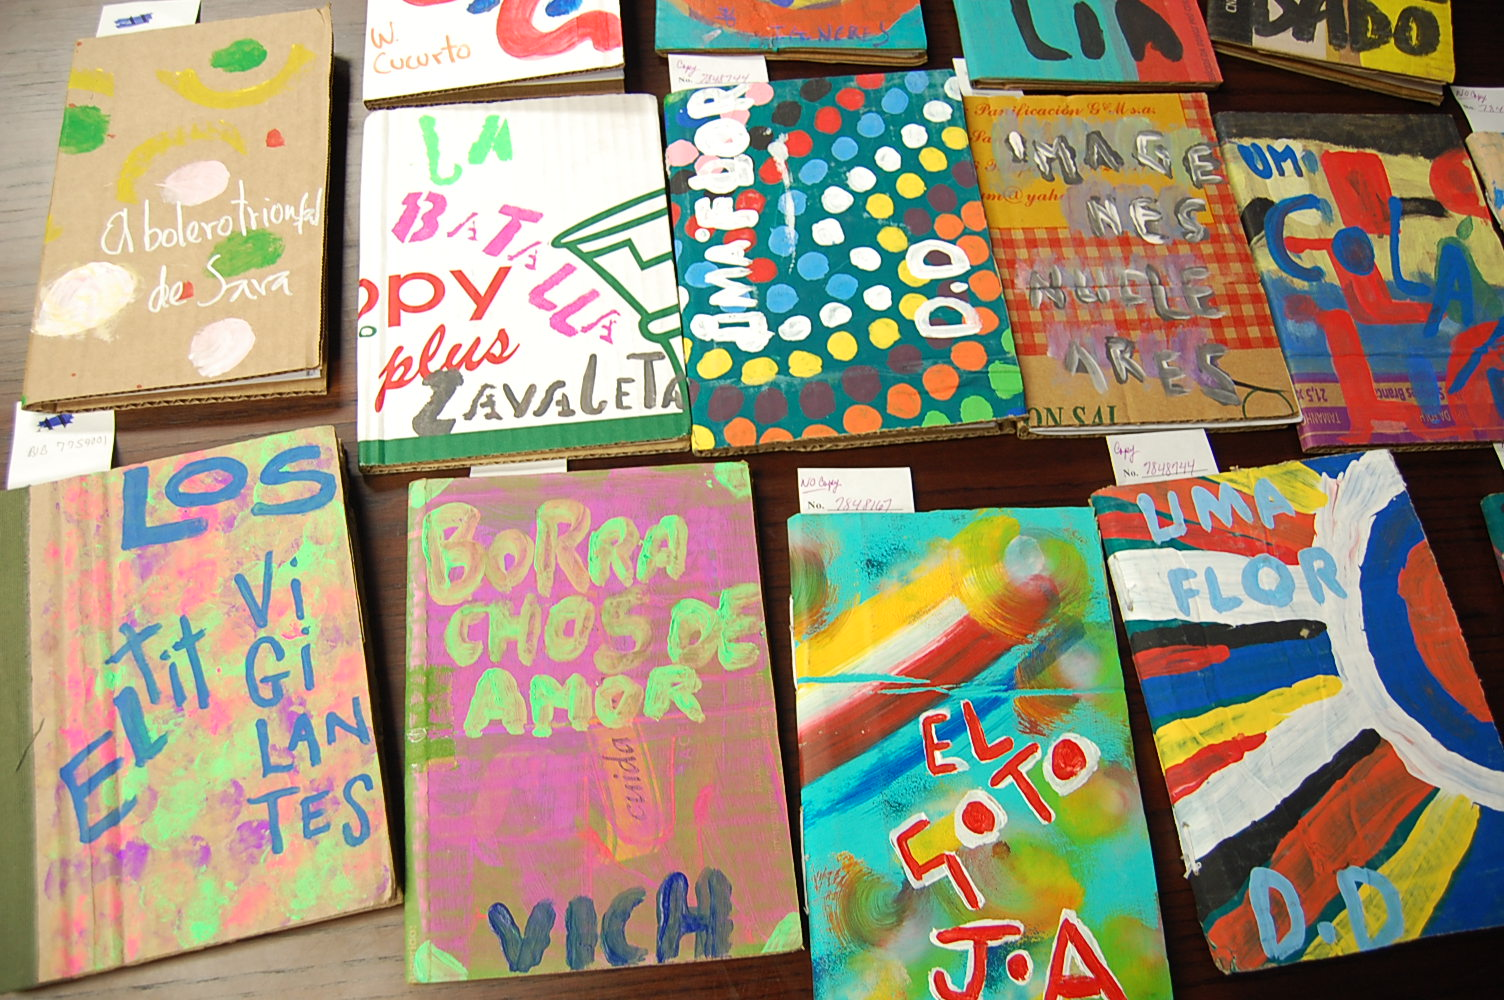
\includegraphics[height=6cm]{graphics/EloisaCartonera_Books2.jpg}
%  \caption{Books covered by Eloisa Cartonera}
%  \label{fig:EloisaCartonera_Books}
%\end{figure}

The film American Beauty, which features a long, poetic clip of a plastic bag swirling on an eddy of air yet people find it hard to think of plastic bags as things of beauty. But as a product -- as something created and then unleashed to become seamlessly integrated into the lives of millions of people around the world -- there is a strange allure to them, just as a pathologist can admire the structure of a particularly virulent and contagious virus.

Examples are not limited with these. Even if \quotes{trash is dirty and smelly trash can provide the raw materials for exquisite art---from sculpture to film and beyond.}



% Örnek sadece bunlarla sınırlı değil, daha bir çoğu sayılabilir, plastik poşetinde şiirselliğin yakalandığı american beauty filmi, kamusal alanı dönüştüren sanatçılar gibi.

%
%
\section{The documentary \quotes{The Gleaners and I} by Agnès Varda}
"The Gleaners and I" is a French documentary film directed by Agnès Varda in 2000. The film features various kinds of gleaning. According to the Merriam-Webster dictionary gleaning refers "to gather grain or other produce left by reapers". Varda searches for the historical and current practices of gleaning in rural and urban areas of France. Historically, gleaning is the act of collecting what is left and not profitable crops after the harvest. By combining different fragments through his film, she shows that the act of gleaning also exists in various forms and styles. In particularly she curiously focuses on the (un)familiar people who glean leftover of society. Moreover, it is a self-reflexive film because the director establishes a relationship with the practice of gleaners and her filmmaking practice. Some people glean crops; the others discarded food, and Varda gleans images.

The film is more than a research and document of the lives of many gleaners. It highlights the degree of global consumerism of the modern world and how technological advancements (or industrial (technical, modern) standards) result in waste. Varda seeks the several stages of potatoes from producers to consumers. As she discovers that supermarkets buy only potatoes that fit in industrial standards of shape and size. So what happens to the others? Varda discovers and shares with us the disturbing fact that they are taken back to the field where they came from, by following with the camera the trucks that unload mountains of potatoes. As Rosello notes that "The ‘good’ potato is not the edible potato but one that will fit into a plastic container to be displayed on the shelf of a supermarket." Varda records few people who glean the rejected potatoes from the field, and also she joins them by collecting heart shaped potatoes that fascinate her. Rosello explains that she is collecting not only refused potatoes but also images that are left behind.

\begin{figure}[h!]
  \centering
  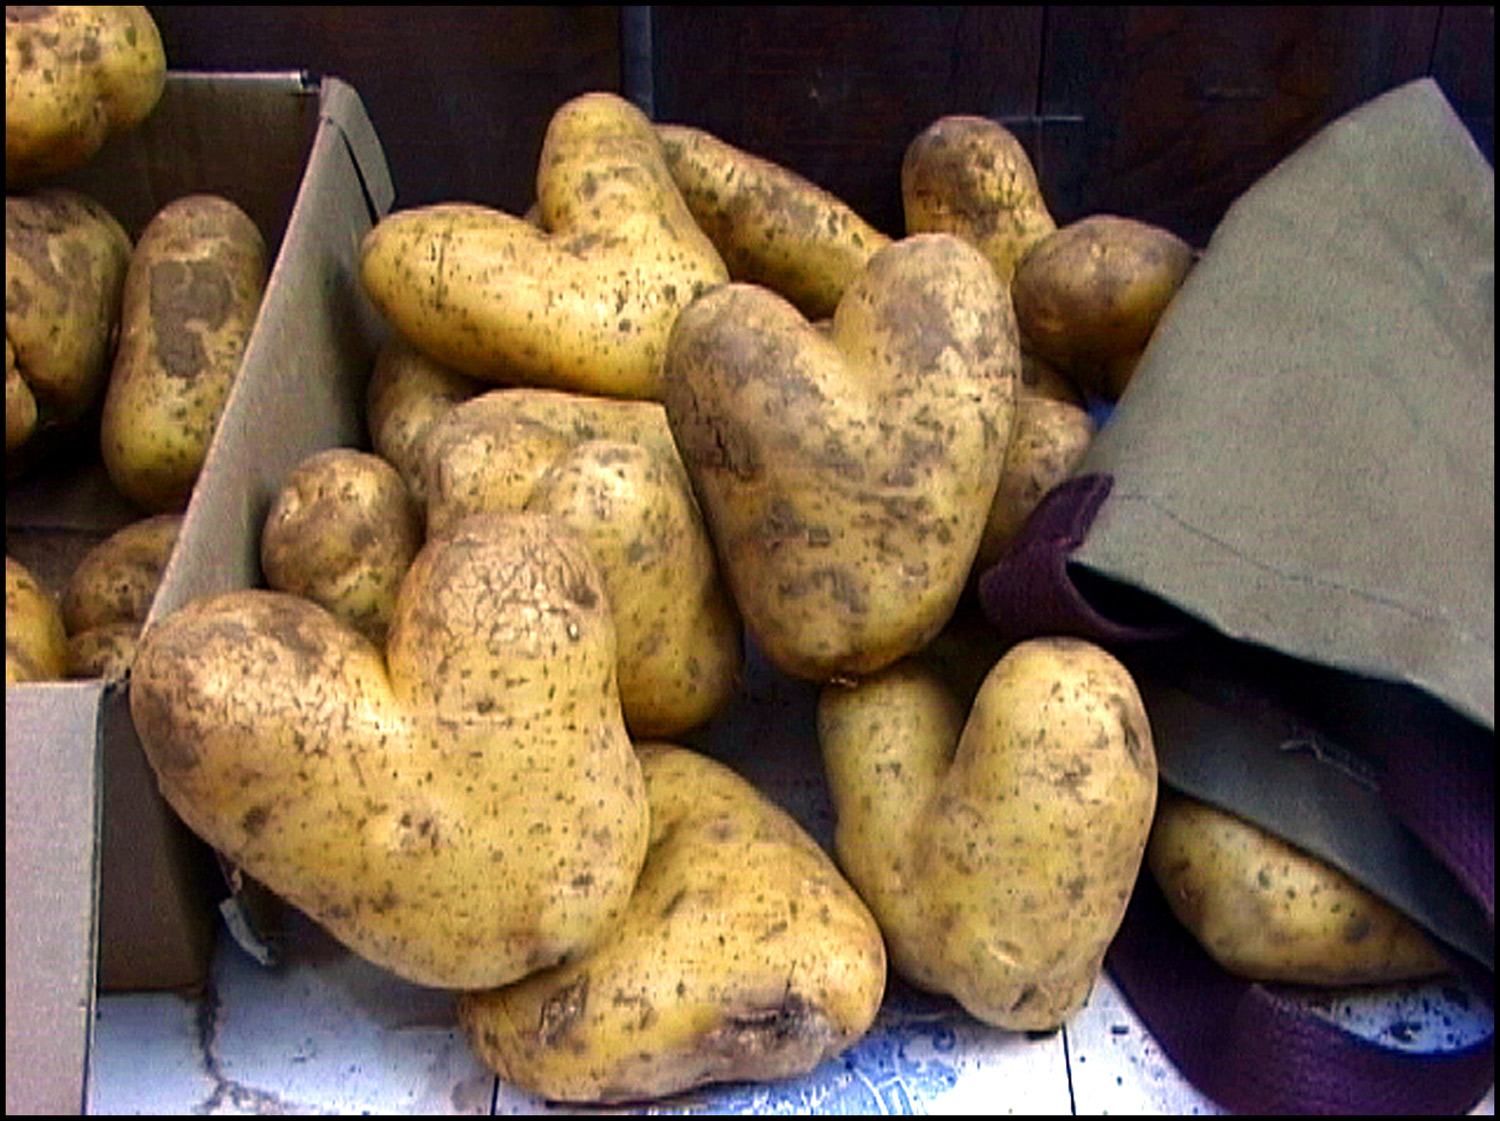
\includegraphics[height=6cm]{graphics/AgnesVarda_Potatoes.jpg}
  \caption{Still image from The Gleaners and I}
  \label{fig:AgnesVarda_Potatoes}
\end{figure}

The industrial processes have some standards and beyond that standards, there is not a place for anything. It clears out (or move away) the rest. It can be viewed as the idealization of goods and products (even people). At this point, it can be referred back to Žižek's claim that people's false consciousness about balanced and idealized notion of nature. It can be understood that this type of clarification of objects may result in this false perception. What Varda's finding is an excellent exemplification of what Žižek wants to point out.

Contrary to the common act of discarding, Varda finds out a creative way to use her unconscious recorded piece that might be deleted by the others. It is the scene where Varda had forgotten to turn her camera off and accidentally films the ground and her lens cap bouncing along as she walks. She uses this scene with a jazz soundtrack at background. Watching this scene is confusing at first hand regarding context. It might be viewed as worthless and recorded by accident. One can ask that why is this placed here, what does this have to do with gleaning? However, Varda forces us to watch it (wants us to pay attention). This scene called "the dance of the lens cap". Ruth Cruickshank in the article, The Work of Art in the Age of Global Consumption: Agnes Varda’s Les Glaneurs et la glaneuse (The Gleaners and I), addressed this scene and clarified the potential deeper meaning behind it. Cruickshank likened the scene to something that is normally thrown away, or in this case edited out of the film, much like the way trash is thrown away or food is left behind after a harvest. \quotes{Where many documentary makers would leave such accidental footage on the cutting room floor, Varda draws attention to how what would habitually be perceived as waste may be viewed as supplement with its own intrinsic value. Rather than literally treating it like dirt, Varda retains and prompts reassessment of that which is normally left out of shot} \cite{cruickshank2007work}. Things that are often forgotten or discarded can easily be revamped to create something useful to someone. The scene was revamped using music, and it became beautiful, much like the gleaners who found fish in the trash cooked it to make it edible, or the artist gleaner who piled discarded baby dolls into totem poles.

%\todo{image}

As Varda demonstrates, people can be discovered throughout the French countryside gleaning everything from potatoes to grapes, apples to oysters, much as they did hundreds of years ago (though no longer in organized groups). Making use out of something that has been left behind and labeled as obsolete is not unique to potatoes. There is so much discarded, yet still-viable food in dumpsters that many people live off it entirely. More figuratively, there are also urban gleaners who salvage scraps from bins, appliances from the side of the road, or vegetables from stalls after the markets have been closed. By showing them she shows that once was a common practice of gleaning throughout the years has evolved, but not disappeared. She keeps light to the modern life gleaners that are not visible every time. One of them is the teacher named Alain, an urban gleaner with a master's degree who teaches French to immigrants. It can seen that from this example, gleaning becomes also a form of resistence to ruling system. a way of refusing to be boxed in by conventional expectations

%\todo{waste and want rules of eating from garbage.}

She shows that the act of gleaning does not bound to the collecting food and survival reasons. Some of them build their own meaning, existence and identity through the collected items. One of the examples that she gaves is that the man who collects baby dolls and use them in the decoration of his home. Every where is filled up with the babydolls even if wall of the garden.

Through the film she experiences the act of gleaning with different people. At one side she gleans potatoes in the field and on the other side follows a man with biycle look for the garbages in front of the homes. By documenting their life in action she also participates their life. But she brings her own perception to them. For example in the case of potato gleaning she collects the heart shaped ones which attract attention of her. Moreover in the case of night searching, she finds a clock without hand. It has fullfiled its function and left away. Most important part of clock is missing therefore it is not functioning. However for her it has a different meaning. Not every time people seek to be aware of time sometimes they want to forget that.

A clock without hands found the garbage pile and taken by Agnès Varda. It does not work properly but it has important meaning for her. The time does not go on and it does not remind her that she is aging. One of the interesting thing is here Agnès Varda feels that as an aging person who will later become a discarded person.

She talks and investigates artists who are using discarded items in the artworks. Which people could not find anything, the artists see countless possibilities. There is always alternative ways to see something different: Giving life or finding life from discarded life. 

Here another point is that Agnes display images of people picking up things from the ground like their ancestors. Everyone somehow collect things in their life but particularlly she selects these people and their images in action. There should be a reason for this! For some individuals, gleaning is not a novelty or a clever way to save money, but a necessity of life. They require it to sustain their life. Combine the elements from different peoples that seems totally unrelated gains powerful theme for the documentary. What gleaning means become more open (or powerful). It draws a picture of body combination of different parts (connected, dependent to the each other). The reason of gleaning varies but the fact that gleaning is continues in different forms.

She discusses the importance found in the meaning and purpose of art forms like this: \quotes{Varda seeks to encourage viewers to consider what potential agency is demonstrated in the artfulness and contingency of gleaning by individuals excluded\ldots from the homogenizing systems of global consumption} \cite{cruickshank2007work}. One can find more treasure in trash than many of New York’s finest galleries and art exhibits; they bring a grassroots feel to what has always been seen as a stuffy and prude aspect of society.

Varda's other subjects include artists who incorporate discarded materials into their work, symbols she discovers during her filming, and the French laws regarding gleaning versus abandoned property. Varda also spends time with Louis Pons, who explains how junk is a "cluster of possibilities." Louis Pons (born 1927) is a French collage artist. He specializes in reliefs and assemblages made entirely from discarded objects and junk. In Agnès Varda's documentary The Gleaners and I, Pons explains his artistic process and understanding of art; what others see as "a cluster of junk," he sees as "a cluster of possibilities;" and that the function of art is to tidy up one's inner and exterior worlds.







%%%
%%%
%%%
%\section{Summary}

% FROM drink UP, author: Werthan, Sarah, artist: Leech, Gwyneth. A Year in Cups. http://gwynethleech.com/
% trash and art collided. Paper and art, actually paper already medium of art, but is there anything different here. Itself is a part of a work, not the drawing, or painting.
% Documenting via a blog or a website. (what type of dimension it brings the work? maybe connect them, leave message.)
% Buying a beverage is a daily event for \ldots
% Creating art in public places can demystify the process for passers by, Leech says, making artistic expression more accessible and part of people’s everyday lives. The reason of website.
% “People see that an artist can make work anywhere, and make creative spaces anywhere,” she asserts. 


% TODO PRAP. from rethink, reimagine, reinvent
%\paraphrase{Recycling art approach to using reclaimed objects in artworks requires rethinking, or examining the affordances of a particular object to explore the possibilities for the object's inclusion in an artwork. Assemblage art involves the creation of new and innovative objects from what were once considered objects of waste; that is. through their use in assemblage pieces, reclaimed objects are endowed with a new. sometimes paradoxical meaning. The transformations of the objects used in assemblage pieces ask viewers to reconsider the notion of "valuable" as they are challenged to look at everyday objects with a new perspective (Taylor, 2006). Viewers confront issues relating to the functionality of objects during modern processes of production, consumption and distribution.}





%"Garbage art (alternatively known as trash art or recycled art) is art created from materials including post-consumer and other waste, collected debris, or objects previously used for other purposes." "Creating art from garbage involves transforming the meaning of objects by placing them in new, aestheticized contexts. This practice is not new; tribal peoples have adapted bits of trash from industrialized societies into their traditional arts since coming into contact with products of the developed world." "Creating art from trash involves “consuming” garbage in the sense that artists appropriate and rearrange the materials in personal ways, transform their meanings, utilize them to their own ends, and represent them in new ways.It involves taking unwanted materials out of their “waste” context and recontextualizing them as “art.”" \cite{tauxe2012encyclopedia}





%
%
%\textbf{What might be the meaning of using trash as a medium in the artworks? Questioning trash as a medium for artist}
%\begin{itemize}
%\item Some works try to raise awareness the problems that are the result of trash. (It treats environment and nature.)
%\item Some of them reflect people's lifestyle especially throw away culture. As a mirror of current lifestyle.
%\item Try to find a new value and meaning from the discarded material that are useless anymore. To explore a new approach, new way. Subvert people's ideas about trash and their attitudes by turning materials to the something meaningful (or valuable). Trash to treasure.
%\item Using discarded item to represent other discarded things by the ruling ideology or approach. For example, trash can be used to represent refugees. The things that we are trying to discard does not mean that they have no value, instead it means that we have no ability to reveal its potential. In other words, refugees have potential but we see them as players that will change our current system. Therefore, it can be said that willing to transform trash to treasure is to require change of current lifestyle. Rejecting discarding something especially thing that you get value from it is a process and spread through to the ones life.
%\item One way is not to produce trash. (Zero trash philosophy.) The other one is to transform trash into something else.
%\item What type of experience is that collecting and working on objects that are generally discarded? Experiencing out of common practice, being open to new explorations.
%\item Instead of a world that produce trash, how could it be a world created from trash?
%\item Combining industrial goods with objects transformed from trash is another way to find a place to trash in the community. It also signifies that trash still has a good quality to used with new materials. Creating composite products from new and reused items. Using the valuable thing with the invaluable thing. It becomes more valuable or less valuable. Depends on the perception.
%\item Aesthetics of trash. Revealing aesthetics value of discarded stuff. (Unique visual value. Trash portraits, sculptures etc.)
%\end{itemize}











% Sanatsal bir eylem olduğuna nasıl varacağım peki? Çünkü topluyorsun, belli bir yaklaşım geliştiriyorsun. Bu eyleme insanları davet ediyorsun. Sanatın eylem olma olayı... Buna burda değinip, kendi işime geçmeliyim.

% TODO From Beautiful Trash Art and Transformation BY PAOLA IBARRA, ReVista
%Recycling has always been a common practice in the arts at least at a non-material level. From creating a world of words in literature, to rhythm and images in poetry, sampling in hip hop music, representation in the visual arts, or editing the illusory continuity of a film, art implies taking disparate elements (ideas, images, references, objects, etc.) and putting them together to form a new whole. Take and put. De-contextualize and re-contextualize. In that sense, art, as a system, is an act of recycling [from PAOLA IBARRA]. 

% TODO new comer
% FROM Book: Recycled, Re-Seen: Folk Art from the Global Scrap Heap
%\summary{Resistance} 
%\comment{Resistance, tactile, agnes varda?} If it is ultimately romantic to speak of these toys (or any other modern-day recyclia) in the language of resistance (by which I mean self-conscious political opposition), I would agree with Marshal Sahlins's assertion that "whether or not it comes to this [resistance], the indigenous mode of response to imperialism is always culturally subversive, insofar as the people must need to interpret the experience and they can do so only according to their own principles of existence. (sahlins 1992, 16)"

% TODO new comer
% FROM Book: Recycled, Re-Seen: Folk Art from the Global Scrap Heap
%\summary{Ironic}
%\comment{IRONIC, maybe added to results of transformation, reusing trashed items in different contexts.} This misuse the detritus of the industrial age has been described by western theorist as ironic. the irony is often embodied visually and conceptually. opposite of natural use, expected perception. for example making something from nothing or turning trash into treasure. By juxtaposing different materials changing context and place. 

% TODO new comer
% FROM Book: Recycled, Re-Seen: Folk Art from the Global Scrap Heap
%\comment{People applies their own perception to interpreted the items.} Human manufactured never envisioned possibilities seen by people. It suggests a self-confididence and intellectual authority that allows local peoples to encompass western goods in their own meanings "in their own scheme of things." 
\chapter{Thesis Project: Notebooks from Trashed Papers}


%****************************************
% Structure of Chapter:
% 
% Artist Statement
% Development of Work
%  Collecting, Transforming, Tests...
%
% Final Work
%  - Notebooks
%  - Website
%  - Exhibition
%........................................


%****************************************
% Relationship between my project and theoretical aspects:
% - First one is actually is to analyze what is trash? Because I am using trash material and what is point of view of scholars to the trash. Realizing the potentials of it. Also the difference comes from the working on virgin object and trash object. Understanding the difference between the bricolouer and engineer. If trash has multiple life than these research will somehow reveal it. It is actually research on trash but what purposes. I guess it is missing? I need to set a purpose for the theory chapter. Or it is a just a background chapter? 
% - Roots in the art history. (Also roots on the social life can be researched?)
% - Inspiration from the other artist and also 
%........................................


%****************************************
% Sample Phrases
% \ldots is the concern of this study which aims to \ldots
% The aim is not to practice Antiquarian Avant-Garde techniques as a puritan form of photography, but rather to envision new means of photography.
% The aim of the thesis paper is to historically, socially and theoretically contextualize a student's work. The written thesis documents and informs the development and resolution of each student's artistic practice during the MFA program.
%........................................


% FROM Wild Art. quote taken from the television series `American Masters', Season 5, Episode 8, John Cage: I have nothing to say and I am saying it (aired on 17 September 1990).
\epigraph{The first question I ask myself when something doesn't seem to be beautiful is why do I think it's not beautiful? And very shortly you discover that there is no reason. If we can conquer that dislike, or begin to like what we did dislike, then the world is more open. That path ---of increasing one's enjoyment of life--- is the path, I think, we all best take: to use art not as self-expression, but as self-alteration; to become more open.}{\hfill---John Cage, \textit{Wild Art}}


In this chapter the artwork(thesis project) will be explained in detail. Final work and it's progress will be explained. Connection will be established with the previous chapters. Stages of work and concerns will be explained. 

% What I have write is here to cover the project can not be sufficient. Because it is not possible to say everything about this project. I wish that this work would allow different interpretation and readings. 


% TODO
% Felix Gonzales Torres'in untitled işi benim yapmaya çalıştığım ile ilgili.


%%%
%%%
%%% 
% TODO
\section{Artist Statement}
(Collect, Save, Transform, Spread.)(Rescue, Revive)

% Closest waste bin is actually my own pocket.

% Converting disposal things to multiple time usage. Realizing the alternative lives of trash beyond their defined one shot life. Giving attention to the things. 

% Eğer bir artistic actten bahsediyorsak sadece bunun ürünle değil, üretimi ve insanların dahil olmasıyla desteklenebilir. Zaten toplama sürecinde bunu insanlarla ilişki kurarak yapıyorum. O insanlarda diğerleriyle konuşarak yapıyorlar.

% At this stage it is claimed that the process of transformation of trash can be treated as artistic act. In the production of notebooks people collected papers from different places and location. During the collection phase they also collect them from other people. In other words there is human communication during this process.

Actually (It is questioned that) working with trash dictates a life practice and, it is a convergence of behavioral patterns (attitudes toward to trash) and art making. The process effects one's life and lifestyle. (But what type of interaction between life and art making process?) (This claim is the main driving force of my artwork which is part of a thesis.) The purpose is not to build a thing that is produced from discarded material to watch it from a distance. The important thing is to interact with it. Because it is already discarded (disgusting, abject, unattractive etc.) and general behavior avoid from it, this work must change it. It must call the viewer to interact with it.

% Ersan hoca uzak seyretmek yerine etkileşime geçilmesini auranın kırılması olarak bakıyor. Performatif olması veya bir act olması zaten bunu kıran bir şey olabilir. Sanatsal eylem, performans kavramlarını araştırmak gerekli. Uzaktan seyredip hayranlık duymak yerine ilişkiye geçilen bir hale getirmek çöpü. Amaç bu aslında. Çöpü tekrar tanımak, onunla barışmak, onunla yaşamak. İşte bu yüzden bir eylem olabilir. Ya da yaşam pratiği. 

% Olay sadece böyle çöpten bir şeyler yapıp insanların seyretmesi değil, mühim olan onunla iletişime, ilişkeye geçmek. Yani zaten uzak durulan bir şey, onlardan bir şey üretildiğinde izleyici gene uzağında duruyorsa ne anlamı kaldı ki? İnsanların bu işin aşamalarının bir parçası olmalılar.

With the help of art (and artistic practices) discarded things can find a place in the society. (By the help of artistic approach things can be gain new values and meaning even if they are discarded and excluded from daily life (or society). The relationship between value creation and artistic practice examined through the artworks that uses trash as medium.)

% Using trash can not only understand in ecological perceptions, it also have powerful political claims. Or it should be examined in deeper levels beyond collage and assemblage, the medium itself has different meanings. 

% SEEING IT AS A RESOURCE.
Junk(or trash) can be seen as a new resource that is fertile to new meanings, creations and aesthetics. Ignored and discarded nature of garbage when rethought becomes fertile resource. Trash as a resource (as an artistic material). (City as a resource. Seeing the discarded items as a resource. Many artist approach to trash as resource. It is a shared approach. Some of them collect city discard, some of them tea cups, tea bags, discarded papers.)

% Çöpü tekrar ele alıp bir şeyler üretmek, onu tekrar yaşamımıza sokmak yeni alternatifler sunacaktır.

Do she/he want to take back (or revisit) the trash once thrown away? People do not want to think of what they throw away. Turning them to a things that worth to look again. How do artists reflect garbage and what are their tactics? What is the thing that add value to trash and what is the role of art in that?

With the help of art discarded things ---in the scope of thesis in particular paper trash--- can be transformed beyond the other industrial (or technological) methods. In other words autistics practices generates applies different methods.


%%%
%%%
%%%
%\section{Inspired Works}
%There are some works that inspire me a lot when developing the work. They are not actually trash related works therefore I put them in different section and here before the details of my work. However the previous chapter has also very inspirational contributions to the my work. They helped the understand the topic and develop an approach to the topic. In this section some projects are mentioned and their methodologies are explained. How are these works effected my work. What is the relationship between them? (Maybe all of them can be explained only the related part of it.)
%SketchBook Project. Inspires me a lot. Lots of works from all over the world. Full of creativity and showcase of richness of people's expressions on the small notebooks. My work can be considered as a sketch book project through trash. Sketches or only creative progress is not the only consideration. You can send your lecture notes. 


%%%
%%%
%%%
\section{Development of Work}
Here stages(progress) of my artwork are listed:

\begin{itemize}
\item \textbf{Memories.} As far as I know I collect things it is hard to say collecting started after an exact event or time but there are several memories that I remember. One of these (First of them) is from my primary school teacher. When I was third class my teacher give us a homework to bring colorful paper to make something(whatever it is I don't remember). The day after we bring some colorful paper but she did not. Instead of this she bring paper cut out from packages that are colorful, shinny and qualify. And I remember clearly that she suggest that same for us. Do not throw out packages, look for the useful parts and keep them to use later. 
\item \textbf{Motivation.} I can not throw them away. When I throw them I became sad for them. I have to find something useful for it. Even if I can not find it, I can pass it to another person who can make use of it for own purposes. We are humans that can produce, transform items. One of most developed species in the earth that produce and use tools. There is a lot of effort to produce thrown away and it seems that all this efforts are wasted. What I mention is not related about ultimate productivity. It is more close to being thoughtful, and taking responsibility of tools, items and objects that we are using. Rather than throwing out, creating a way that all are have chance to live together is much more close to my perception. 
\item \textbf{Collecting.} One of the most found trash in my habitat is paper. I work at METU Technopolis, live at 100. yil which is the nearest settlement to METU and study at Bilkent. People live there commonly use paper and needs paper. Paper is nearly everywhere. Reusing the paper is not limited with recycling of it. There is a another ways of it. When we recycle them actually we again send away them and use it as we all know. (industrial papers and notebooks.) There is no richness here. Same type of paper. Produced after a industrial process. I collected them from my friends (people that have communicate often). Sometimes I collect them from trash bins and roads. 

\comment{COLLECTING TRASH.} One of the most important parts of the using trash in the artwork (or expressing something, or representation) is to collect them. What are the dynamics(considerations) of collecting them? (easily accessible materials or unique items.) Where to store them? Does it mean that live with trash? In other words collecting trash and using them is live with them? (making them part of life.) After the being part of the are they still trash? Can be thought that it is something that affects the lifestyle. (possessions and trash.) Another question is that how differs collecting trash from collecting other things such as objects that have archival value. What is the driving force? You may collect it to prevent object being lost. For archival things what you collect is something that has some sort of social use and meaning which is going to disappear. However, trash is never disappearing, even its amount increasing rapidly. For archival things people have memories with them, but does some applies for the trash? Who wants to keep trash? or who wants to re-see(re-visit) trash again (in a museum for example)?

\todo[inline]{What type of collecting? How differs from the others? ragpickers from benjamin and archades project.}

\todo[inline]{yaptığım işten diğerlerine referans vermek gerekli.}

\item \textbf{Transforming.} I turned them to notebooks. Actually I use it for my self. And while I was using of it I am very proud of it. I am studying nearly more 20 twenty years and I have always need for notebooks and use them. It is some sort of passion for me notebooks. Because I always admire notebook beautifully design or uniquely designed. I collect them whenever I find and most of the time I only save them for later use. 
\end{itemize}

\subsection{Collecting}

[Organazing People] Well I  actually follow very simple methods. I just talk them all. I explain what I did, ask for their help. Everyone actually approached positively and somehow they contributed the project.

\subsubsection{Collected Materials}
There are different papers and objects are used to produce papers
\begin{itemize}
\item Burger King packages, from office at launch time
\item Starbucks packages, from supervisor, office and my friend. Especially my supervisor and friend collect them from their friends and their own uses. They save them for me and later I take them later. 
\item Modshifters papers, that are covered on table and at the end of the day they are cut out and throw away. I go this place many times and every time questioned what they are doing to the papers. One of my visit we stay there at a late time and catch the garson collecting the old papers and prepearing tables to the next customer or day. I ask him to give me and he kindly accepted. From this paper I covered [x] notebooks. All of them contains track of people who sit down there. I do not know them and I am not sure that the paper that they are sit down turned to such a thing. 
\item Varuna Gezgin
\item Graduation banner
\item Tea bags.
\item Banka sıra fişleri.
\item Elginden gelen kağıtlar.
\item Bilent kağıtları?
% It is also realization of materials. Establishing different connection to them. Why is important? Identity construction.
\end{itemize}

\subsection{Experiments}
\todo[inline]{experiments with paper.}

[EXHIBITION] Starting point is to stack the notebooks onto the each other, and there are some ideas like putting them inside a waste bin to re-do the action of throwing away. Again the purpose is to find a way that to shock people, surprise them. After ward somehow they should understand that these notebooks can be taken. \comment{I set up makets and try some installations of it. Take photo it. listed them here.}

\todo{images are here.}

I imagine a exhibition environment and place notebooks \comment{üst üste.} Different placement are tried. All of them are look like sculptural. I have insert no special meaning as sculpture to this object an I also I am afraid that people does not close them to the notebooks and look them away. which I do not want. 

\todo[inline]{bir de aynı zamanda işin süreci, defterlerin yapımları hakkında bilgi vermem gerekli.}

%%
%%
\subsection{Problems}
There are a lot of questions and problems that I have to overcome while development of my work. 

% Yani aslında bir derdim ve yapmak istediğim bir şey var. Ama bunu gerçekleştirmek için yapmam gereken şeyler var. Ve bunların bazılarının nasıl yapılacağı çok belli değil. Ben bunlara bir çözüm buluyorum. Bir yöntem üretiyorum. Bu kısımda aslında bunlardan bahsediyorum.

\begin{itemize}
\item First one is that my art work can be considered as design and has functional purposes. (It is not just a design, it is uses design to reach its goal like many artworks use other disciplines to reach their goals and expression. Purpose is not design and functionality.)
\item Using unused industrial paper. (Mixed trash and virgin material, \textbf{to show that discarded and desired object can live together.})
\item Collecting them with help of people, and asking other people to give the unused papers. (Collected from my close friends, from supervisor, from office where I work, from modshifters and varuna gezgin and from bcc labs(hopefully)?)
\item Giving them to people, but people should take them voluntarily.
\end{itemize}

\subsubsection{Functionality and Art Debate}
From an art historical perspective, you could say that functional art is the inverse of Marcel Duchamp's famous readymades, where he transformed utilitarian objects---a urinal, a bottle rack, etc.---into conceptual artworks by fiat: it became art because he said it was. Duchamp's works kills the functionality. It works beyond the functional perception. Moves the debate to the conceptual frame. However it is not every time case. Today many functional art objects are as avidly acquired by collectors as their fine-art brethren, and are appreciated just as much for their beauty as their use value. Ancient Chinese vases, for example, while still capable of performing their originally intended function (displaying flowers), are prized for their historic and aesthetic value more than anything else. \quotes{In conceptual art,} Sol LeWitt writes, \quotes{the idea or concept is the most important aspect of the work\ldots The idea becomes the machine that makes the art} \cite{lewitt1967paragraphs}. Therefore anything can be turned to art with a good idea. 

\comment{Comparing art to craft is like comparing philosophy to engineering: they're two separate ways of looking at the same thing. To me art is communication of an idea or an emotion, while craft is the physical manipulation of material. An object can easily be both, either, or neither. A sculpture, for example, may communicate, but it was constructed using craft. Likewise a teapot can communicate an idea, but it was crafted. Function is misleading and no distinction. Functional objects can still communicate ideas, so art can be functional. One object could be viewed two ways: if you look at the way it was made and the materials used, you are looking at its craft, if you think about its ideas, you are viewing it as art. An object could have been crafted, but contain no art. Even a painting can be crafted but artless. A ready-made might be art with no craft. I very much like the idea of a spectrum. One last thought: skill doesn't enter into the definition of art, since a piece could succeed as art but be poorly crafted.}

\textbf{Why is it not a design?} Because the considerations and priorities are different? Functionality is not my primary concern. I do not increase the functionality or searching best functionality? (Considerations of design and art can be compared and what are my priorities in this work. I'm not trying to finish the garbage problem. Is it a problem for me? Do I problematize it?) 

\textbf{Why is it art?} Uses artistic methods? Does it represent anything? The idea is transforming things. Anything can be transformed and re-contextualized again. The limitation is our imagination and approach. It has a claim. In can be analyzed and examined in the context of art. It is hard to say that something is art or not. However it can be examined in the context of art. There are artworks reject art galleries. There are artworks also reject commodities. It has purpose that. spread out the idea in different manner. Subverts peoples ideas. 

The work aims to liberate the imagination and change the way people see the trash.

%%
%%
\subsection{Paper}
"Paper is an indispensable product throughout the world. Its primary use is as a medium for writing, essential for bureaucracy, education, communications, information storage, and in the spread of information. In addition, it is used for the packaging for transport and convenience of a wide range of items from food to industrial equipment. Paper also has specific technological uses, such as for filters and in art, home furnishings, and architecture, and it has a range of uses for hygiene purposes. Paper in several forms is consumed on a daily basis by each person in the Western world." \cite{trafford2012paper}

\comment{My experience here: For example when i collect the papers under the dishes or food packages, people often thinks that it is disgusting and call them as dirty. But it is very strange that the fat on the paper is previously what they are eat.}

Paper is both biodegradable and a renewable resource, which means in consumption and waste terms, its environmental impact is relatively small compared to the many more-toxic and bulky waste products that are found in everyday garbage. However, the chemicals, water, and electricity used in its manufacture are considerable---and these are nonrenewable resources---and certain types of chemicals used in paper production are toxic. In addition, if waste paper is sent to a landfill, it releases carbon dioxide emissions. Further, forest resources are not always as renewable as one may like to think. These environmental impacts can be greatly reduced by recycling (paper being one of the most easily and cheaply recyclable products in everyday use) and by conscientious consumption practices.

Paper made exclusively from wood is called virgin paper, while paper produced out of used paper that is re-pulped is called recycled paper. Recycling paper can greatly diminish demand for virgin fiber from wood. However, there will always be a demand for virgin paper because, although paper is thought of as a renewable resource, it cannot be recycled indefinitely. It can only be recycled four to six times, as the fibers get shorter and weaker each time. In addition, some virgin pulp must be introduced into the process each time to maintain the strength and quality of the fiber, so no matter how much is recycled, paper will always need some virgin fiber.

% History of Paper
The word paper comes from papyrus, the plant that was first used for making a medium for writing in ancient Egypt.

% Production of Paper
All types and qualities of paper share the same basic method of manufacture, including newspaper paper, print paper, and carton used for boxes.

% Uses of Paper
Paper has become the most ubiquitous product in the age of information. Such products often complete their journey from shop floor to garbage in a single day; for example, newspapers, print paper, packaging, lavatory paper, tea bags, transport tickets, price tags, shopping bags, flyers, leaflets, wrapping paper, napkins, and tissues. 

%%
%%
\subsection{Why (package) paper?}
Easy to collect. Easy to find. Thrown out even if it is good quality. Packaging materials are very widespread. Appropriate for painting and writing. Has a very short life time. Disposable, there are a lot of package outside. No need to carry it. Every place gives you package paper. 

%%
%%
\subsection{Why covering notebooks and books?}
They are all package paper, already used as carry things and this work it has used again for the same purpose (but in different connection, this time trash is bound to the notebook). Trash is used to cover the papers. Cover is the most visible part of the notebook and book. Therefore trash becomes most visible part of the produced item. What is the function of cover? It gives ideas about what is inside, distinguishes from other things, protect it.

%%
%%
\subsection{Why giving away?}
Aim is to spread the idea by making something useful from trash. Increase diversity, activate (or encourage) people to embrace the trash.

%%
%%
\subsection{Why in the public space?}
To reach more audience. Actually the audience is out of the art galleries. They are walking in the streets. Putting them to next to people is much more effective. It is not visible and nearly it is hided from society. It is dirty. Removed from the society. There is a effort to hide them away. However in this project it is again showed to the society. Because it is revisited and reclaimed. 


%%
%%
\subsection{Artistic tactics}
Here I followed some tactics to realize my purposes. I called them artistic tactics. Easy to carry while traveling. Small notebooks. Placing them to their routes. 

\subsection{How I reached to notebook?}
Actually I have been collecting same materials that are used in my project before the thesis work. In my mind there is always belief that I can I find something useful for them. (In that time my main evaluation was to create useful object for my need.) Later it turned to an artwork. Before the thesis I also produce the notebooks for myself. However what is changed in thesis. First my approach to the trash is a little bit deeper. What is added to the notebooks. I started to use also used papers. for the cover of the notebook, I use more different materials. more close to collage. production method changed. and I started to collect different things, from different places. My realization increased. I organized my close friends and others to collect or save their trash for me. I discovered some points. their differences. 

% What I tried during this progress: Wrap out the trees, because I think that most of the materials that I collected are package papers. Well I somehow package the trees again. not to carry them but to raise awareness. Yani benim amacımı en iyi anlatacak olan şey nedir? Aslında ben burada defterden gidip bunu anlamlandırmaya çalıştım. Dolayısıyla deneyerek deftere nasıl ulaştım da ziyade defterden başlayıp nasıl tekrar defterde karar kıldığımı anlatan bir hikaye olabilir? Yani bu çok da şart olmayabilir bir diğer yandan da? Developlement of work? Nasıldı nereye geldi? How my project evolved? And this also explains how it is relates with the research. Because the reasearch is shaped the project also. Which part of the project shaped by the project? Not thinking in the ecological perspective. Raised questions also mature the project? For example zizek suggest that to find spirutuality and aesthetics to the trash, and for me? 

\textbf{Why notebook?} Because I already do it. So What I didn't change it. It is the best one or no to change it. I love idea of carrying notebook with near of you. I have also save my notebooks. I don't throw away them. A notebook is actually is a work of you. It carries your signature. It is one of best gift to give someone. Because it is a combination of your work and the other peoples works. It is co-authored work. Actually there is also a part of people who throw away this peace. Actually the best part of it the transformation is not finishes after my creation of notebook. It continues with the usage of it. How it turned to is not actually uncertain. Therefore it is very appropriate of my idea that transforming trash is increases the diversity.

\textbf{What is different from industrial notebooks?} Handmade, from trash. an alternative to other versions. every one have different stories, they are different in visuals (but the others are also different.) What makes them different is not clear actually. Does it have to be different? Yes. The production method is different. You pay no money. There is different with gift notebooks from companies. This notebooks call to you change the destiny of trash together. 

\subsection{What do I think about trash?}
I need to clarify my approach to the trash, wasting and discarding. First point is that I am very uncomfortable to the action of discarding thing. I always think that by discarding this think I am missing something rather than getting rid of something. Sometimes because of the significant amount of residue from consumption from daily activities I became overwhelmed and to move on I need to leave behind them and move on. However almost it is never ending loop. (I believe that sometimes we need to break the loops to realize different meanings. To think outside the box, we need to behave outside of common habits. As I mentioned the discarding things are some of the loops that we are rare to behave like other way.) \textbf{What am I discarding?} To get rid of my load and move on. But for what? and also ought to be like that? (throw away them to same bin. (Some of people do not care too much bin and throw them whenever it is possible.)) Even if I discard some stuff I think that I am ignoring its potential and losing it. At that times I become very sad and feel very comfortable. I must have find to another place for it more suitable than a waste bin. At least I can give them someone else who can use it for own purposes. Do I really luxury of discard?

Significance of thinking outside the box (about actually trash) is actually breaking the loops. You have to look at differently from your common perception. \textbf{Break the rules, break the loops.}

\textbf{Making exploration.} One of the encouraging factor is to work on trash is to find (or explore) something different from someone else's discard. Because it is discarded and undiscovered. Wait us to be discarded. and possible (as picasso mentioned) discovered again and again. 

\section{Parts of project (or final work)}
The project introduced in this thesis have different parts. Each of them are connected to have relation with and support the other. Different parts also enable us that different level of integration to the project. 

\subsection{Notebooks}
Mixing materials is main method in the production process. I combine different papers and packages. I try to generate every possible combination. For some of them I establish the connection but for the others the connection is not obvious but it is not obligatory. Because trash is state where you can find meaning through the trash or material later. 

All package papers are cleaned up. Because it is important that it needs to be safe to use. With mix of water and little bleach they are swabbed. 

\subsubsection{Name of notebooks}
  \begin{figure}[ht]
      \centering
      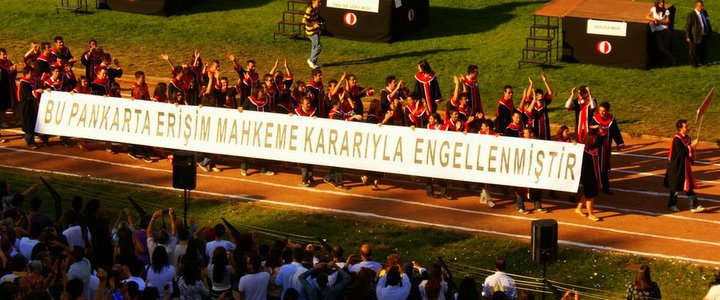
\includegraphics[width=0.8\textwidth]{project_graphics/banner1.jpg}
      \caption{Banner}
      \label{fig:Banner_1}
  \end{figure}
\begin{itemize}
\item \textbf{Puzzle.} Because it is cut out from very big and long banner (which is carried at graduation ceremony at METU, 2011). Every piece was a part of bigger banner. At that time there are serious debates about freedom on the internet. Most of the website are banned from the decision to the courts and they were not accessible. (Access to this banner is blocked by a court decision.) In Middle East Technical University there is a tradition that in graduation ceremony people walk through in the stadium and greet to the tribunes. With this event they carry some banners to express their feelings and criticize some realities in the country. This one of them. It is carried by students (new grads of Computer Engineering) The slogan decided by among the students and before the ceremony I printed out the slogan to carried out as many people as it can and easy to readable from the people who seat at the tribunes. After the ceremony I could not throw away this banner. I do not know what to do it, it is very big actually to store but I could not. I think that I will figure out later. Maybe I can use it as a draft paper. But is it worth to cut out this all long banner etc. Also to strengthen the banner and to prevent to tear while carried by the many people we are tape it from its boundaries. In other words some of the areas can not appropriate for writing. When I decided to this topic I remembered to this banner. It is stands in a corner in a dusty way. Now it is time use it. It waited very log time and it is time to revive again. Currently In turkey the problem of banning web-sites continues. Event it can said that people do not surprises when a website is blocked by the courts. It can be turn be a paper that people can freely express their ideas and feeling onto the it. Cut out them to the smaller pieces and make them as notebooks. They are part of puzzle. for the smaller parts what is written on them can not easily understandable. To realize what is the message is you have to bring together all of them again. But It is not possible, therefore website is a very good solution for them. All pages have unique patterns. Remaining parts of letter and tape. It provides unique layout for writing and I strongly think that all the notebooks after used have strong visual impact. 
\item \textbf{12:00 pm.} Burger King pockets from office where I work. Because it is launch time. It is collected at the same time.
\item \textbf{08:00 am.} Breakfast time. I think that these packages are used at the morning, very the beginning of the day.
\item \textbf{Friday Night.} (Maybe there can be another option related with traveling, or union). These notebook's pages are collected from restaurant "Varuna Gezgin". We go there to meet some friends after long time. One of them is coming from Australia, the other one is coming from Norway. they are my friends from the university. We united again at varuna gezgin. The place also interesting story. It is a place of travelers. It supports them. and the decoration of that place contains a lot of items collected from different sides of the world. The concept of the place and our meeting perfectly matched. I'm collecting the paper that are under the plates. When we are leaving this place, I ask the guy at the desk, I am making small notebooks and is it possible to exhibit there. I said that is it possible to give them to people. Firstly he asked me that selling them but I said no they are free and part of my thesis project. and later he offered me there are a lot of unused papers. I can give you. they are not used and waiting to be recycling. I took some of the papers, and that papers are part the sheets of these papers. 
% Name of the paper can be related with this place and related with the meaning. 
% Again I need some memory from here. 
% They are all my memories actually and I also turn my memories something different. Changing and constructing memories. And also others' memories... These project also contains others memories.

% Ersan hoca's packages. Elgins' papers etc. I do not know actually their stories. Maybe I can dream up stories for them. Creating histories from some of the trashes. They do not have proper memory with me, but I tried to construct memories, (fake memories can be said that.)

% Refer to 9 canlı. Never dies, revives again and again. Because trash moves in the community, even if thrown away can be find another use.

\end{itemize}

\subsection{Exhibition spaces}
Especially it is the most hard topic in the development of the thesis. To find a place for the notebooks is great issue for me? 

\begin{itemize}
\item Library. The reason why select library is there are small papers to write down the location of books. Libraries are places that things are reused. Books are used by many people. It is place of sharing culture. Books are shared by all the other peoples. 
\todo[inline]{problematic because of resusing. actually is sharing.}
Bilkent, METU, Milli Kütüphane. Buraya nasıl gidilecek. Ama öncelik zaten bilkent kütüphanesinde. ODTÜ sonra geliyor. 
\item Torun. as an alternative place?
\end{itemize}

\subsection{Website}
As I think that finding a place the discarded items is one of the main purposes of this project. As it finds a place peoples life again, it also finds another place in the digital space. ()

Mainly websites displays the story(History) of notebooks. Also it is a place to track the journey the notebooks. As I claimed that it is not a finished work. It does not completed transformation. It always continues. Therefore a website that anyone can reach share their progress via website. Anyone can later discover how they turned to new things etc. 

Collect peoples comment with this notebooks. As I leave notebooks different places I do not have connection with people who take them. This website also will help to collect/share peoples ideas about the notebooks.

It will contains a section for how notebooks are produced and the story behind it. The purpose is to record the creative process and share with the others. Revealing the process is significant to demystifiying the truth about the project. It makes it more clear that the object used here is actually transformed from something else. 

\textbf{Why website?} Maybe you can think that there are different methods to accomplish recording and sharing the process. In a gallery on a single table or a room it can be succeed. However it like the idea that website can evolve by time as this work evolve in time. I think it matches perfectly. This is not a finished work, it continues and so the website also. 

% Meaning of stories behind the process
There are different stories behind the objects. I try to record their stories (by photography and taking notes) but some of them were not possible. However I still use them in the work because even if I missed their story, with their materiality reveals their history. It still has a history but needs to rewritten. Maybe forgetting all the history maybe creates different notebook.

It is also co-authored work. Because many people helped me to collect the papers and also many people leave their trail to the paper and also they bring meaning to the them. After production of papers I also want them to continue as co-authored process. In other words many people will be part of this project. As people see different things on objects and bring them to me. the variety of things is increased in time. Because people sad me that \quotes{I thought that you can use it. Do you collect also these?}. After that time I want to continue as so. 

% I add the screenshoots of website. Also the development of it. Sketches of website. Navigation of it. User interaction. Use cases and actions. Functionalities.

% Documenting the progress. 

% It was not only that such characteristic was clearly suited for the exploration of human spaces such as home, but it was also that I am comfortably and confidently fluent in practicing photography

% Counter Argument:
% People may think and raise the question that none of notebooks is actually my work they belongs to others, others(Starbucks, Burger King) designed it and I am stealing their work. Here there are available different answers to the question. Firstly they are different once they are designed. Turned to different thing. I suggest that them to consider in different context like Duchamp. 

% I resurrect things that have been killed off... My work is all about the potential of materials — even when it looks like they've lost all possibilities. (Cornelia Parker) https://en.wikipedia.org/wiki/Cornelia_Parker

% These all memories and collected materials related with the my history. So why is it important for the other people. What can they found my memories. This is not theirs. How other people connect to the topic. They important for me but also I need to find something important for the other people. For example modshifter and varuna gezgin is one of them. This not only my experience. Some kind of shared memories and histories. What will find people in these notebooks.


%****************************************
% EXHIBITION
% Where people access them? How to design the experience here. The relationship with the location? 
% Pizza box, with l shape box. I need to find a place to put them. 
%
%........................................


%****************************************
%% Move to the other sections:
%
% Mandy Barker is an international award winning photographer whose work involving marine plastic debris has received global recognition. The motivation for her work is to raise awareness about plastic pollution in the world's oceans whilst highlighting the harmful affect on marine life and ultimately ourselves.
%........................................


%****************************************
% TODO Find a solution for this problem:
% Bu işin olması için ben insanlardan bir şeyler yapmalarını istiyorum. Yani aslında kendimde yapabilirim ama neden insanları da dahil ediyorum? Buradaki en önemli amaç değiştirmek dönüştürmek, sadece çöpü dönüştürmek yetmez, insanların fikirlerini de deönüştürmek gerekmek. ve bu bir süreç işi (şart mı tek bir yöntem bu mu?) İnsanlar nasıl değişir diye sormak gerekir o zaman. İnsanların değiştiğini dönüştüğünü gerçekten nasıl ölçeceğim ki? 

% important question: herkes neye ihtiyacı var ise onu toplar. ben neden niçin topluyorum. toplama sebepleri. dönüştürme sebepleri. neden sadece toplamakla yetinmiyorum. yani toplamak ile ayrıldığı noktalar nelerdir. Ben bir mana mı arıyorum? Yoksa kaybetmekten mi korkuyorum? Yeni kompozisyonlar oluşturmak istiyorum. Farklı karşımlar elde etmek istiyorum. Bir tür şaşırtmak durumu... Beklenmeyeni yapmak... En olmadık malzeme çöple çalışmak bu yüzden önemli benim için. 

%
% PROBLEM:
% In theoratical part I am focusing on actually the trash. But should I focus on paper trash? Is there any difference? Ya da ben oradaki bir farklılıktan besleniyor muyum? It is not totally paper, actually they are package. Examples can be given related with package material. It has a very short life. Not short actually. 

% How to establish the relationship between the collaboration and the trash? transforming them with the help of people. However, main discussion is not about collaboration. Here collaboration is a method to reach the aim of the project. In other words it is a methodology. There are different methodologies applied by artist to transform them. My methodology is to collaborate with the other people. My aim is to transform trash with people. Also make them to engage with trash. Trash is only one of the things discarded by the society. What is the importance of co-authored work?
%........................................


%****************************************
% Explain your project that I am like and child: 
% Collecting things means actually searching things. I'm searching for materials and also 
% What is the main focus in my work? Participation? Transformation? Composite of them? Trash? What else? 
%........................................


\chapter{Conclusion}





%
%
\begin{singlespace}
\epigraph{If I seem to be over-interested in junk, it is because I am, and I have a lot of it, too --- half a garage full of bits and broken pieces. I use these things for repairing other things\ldots But it can be seen that I do have a genuine and almost miserly interest in worthless objects. My excuse is that in this era of planned obsolescence, when a thing breaks I can usually find something in my collection to repair it --- a toilet, or a motor, or a lawn mower. But I guess the truth is that I simply like junk.}{\hfill---John Steinbeck, \textit{Travels with Charley, 1962}}
\end{singlespace}




Trash is everywhere. Part of our activities. Rubbish as an object state is not static. Its value, usage may vary according to the people. Artistic intentions are aimed to transform the material. Whatever the reason that people are discarding things there must be other type of action that can be able to reverse it. Aimed to create new possibilities from trash.





%
%
Through this thesis many artworks are analyzed. They have differences in terms of purpose and approached to the trash. Some of them only valued from its plastics effects (physical properties). Some of them turned to the performance. 

Their methodologies are different. Their works can be viewed in various dimensions. Their works are also show that the great diversity and the potential usages of trash. 
There are different motivations. 

Reconsidered the notion of trash through the examining the phenonemnons of current age disposable items and ecological concerns. 

There are lots of points to approach to the trash. This shows that our richness of this topic. 











%
%
\textbf{Evolution, Critics} During the process I have also generated lots of trashed papers. Cutting and pasting things also leave unused items. I do not know what to do with them. It is hard to use all of them. Saved for later use. On the other hand being aware of this trasnformation act is very tiny part of the big picture. I can say that my trash is reduced but is it same for the other people. Hard to collect all of them. 

There is also discard is being generated during the production process of papers. How to use them? Need to find a way because varda uses her discarded item inside of the film. Always(or in every proceses) new discard items are generated.






%
%
\textbf{Future Works.} Web site will expand in time. New notebooks from different papers (in terms of location, meaning, usage purpose)

Within the scope of thesis only words that are English is examined but in different languages and cultures there might be different naming for various stages of object and trash. Analysis of them may be subject of another thesis.



% TODO conclusion?
% \comment{ANALOGY Between landfill and graveyards. WHOSE TRASH?} \quotes{There’s a relationship between graveyards and landfills, one that makes us uncomfortable, Zubiaurre explained. \quotes{What is happening to trash is what is going to happen to us. We’re all going to end up in a dump, and we’re going to decompose. That’s the ultimate destiny of humankind, and we don’t want to face that.}

% Buradaki en önemli amaç değiştirmek dönüştürmek, sadece çöpü dönüştürmek yetmez, insanların fikirlerini de dönüştürmek gerekli ve bu bir süreç işi.

\chapter{Uncategorized}

%****************************************
% EPIGRAPH:
% How to cite epigraph http://blog.apastyle.org/apastyle/2013/10/how-to-format-an-epigraph.html

% FROM http://stanforddailyarchive.com/cgi-bin/stanford?a=d&d=stanford19920130-01.2.5&e=-------en-20--1--txt-txIN-------#
% The thing to do is to find some way --- and it can be done, I think, through art --- to enjoy life in its vast multiplicity. --- John Cage

% FROM Wild Art
% Bu epigraphta aslında şöyle bir sıkıntı var, bir şeyin miktarı artınca daha fazla insanın onun üzerinde düşeceğini varsaymak biraz sıkıntı olabilir.
% We are going to make a lot more junk, and there is going to be a lot more junk art. I think people are going to have a lot to say about it, and more people need to think about it. --- Jeremy Mayer, quote taken from American Craft Magazine, December/January 2011.

%%%
%%%
%%%
\section{In Theory}

%%
%%
\subsection{What is trash?}
In this thesis work to understand the different aspects of trash is a key element. Because as scholars agreed on (ref required.) it is part of our life and daily practice and it is very common concepts from developed western societies to rural areas, from disaster areas to \ldots(something beautiful here). Sometimes it is accepted as a problem that is need to carefully and seriously manged. On the other hand it is accepted as a source of diversity. (To establish a solid understanding for trash, it is important to see its dilemmas (it is really a dilemma?)). Therefore we should ask these questions: What is trash? How does it became trash? Is it a end product or a source material? How much is it valuable? How much is it dangerous?

%%
%%
\subsection{Trash is everywhere and, produced every time}
Modern (developed) societies are continuously generating trash and, pile them on landfills. It's a common object category that all people share its possession. During daily activities trash is generated and people get rid of them by throwing away. (Various objects become trash after their primary functions daily. Who defined the primary function? Primary function is the only function. People cares the package of the objects that they buy. They buy the coffee not the cup of it. After coffee finished the life of cup also finishes. There is a lifetime defined (or forecast) by the producer of objects. However it is not bound to the producer, also consumer play an important role. There are different choices. Throw it away. Keep it. Give it. Mostly wining choice is throwing away and by the result of it mountains of garbage are increasing.) The vast amount of industrial discarded items spread through the landfills to oceans. They are the result of highly complex industrial production methods. They are not easily disposable items. They live in the nature thousands of years. Most of them packages that are used to carry or protect other materials. After real material used these packages became valueless (or useless). (types of trash can be mentioned here, but currently in the artwork I'm using paper packages, therefore, it is more important.) How manage the all this increasing trash that damaging nature?  This is the common approach to trash and the main problem. (actually the sustainability problem.) It is not the only problem, It can be thought that it is a losing the ability to transform new things, alternative behaviors etc. (Instead of creating new opportunities or alternatives, it is a consuming all them and producing huge pile of trash.) (reference Zizek idealization of nature, to love nature is to love trash. Live with trash. Do not see it as trash actually. Then the question is how to love trash? how to live with trash? can living with our trash enrich (our perceptions, abilities)? how not to see them as trash and useless? Can it be possible with art?)

% TODO PRAP. REF.
Waste pickers are an important part of the story in Latin America, as more is being thrown away than ever. The World Bank estimates that the amount of solid waste generated in cities is growing faster than the rate of urbanization. The higher the income level and the rate of urbanization, the greater the amount of solid waste produced. OECD countries produce almost half of the world’s waste. Africa and South Asia produce the least waste. High-income countries have the highest collection rates and are most likely to dispose of waste to landfills or incinerators. Low-income countries have the lowest collection rates and are most likely to dispose of their waste in open dumps. However, low-income countries also have the largest numbers of informal waste pickers who collect, sort, and reclaim recyclables---thus reducing costs to the city and to the environment. (FROM Trash as Treasure, BY WILLIAM L. FASH AND E. WYLLYS ANDREWS)

% TODO PRAP. REF.
Literature is recycled material, a pretext for making more art. I learned this distillation of lots of literary criticism in workshops with children. I also learned that creative and critical thinking are practically the same faculty, since both take a distance from found material and turn it into stuff for interpretation. For a teacher of literature over a long lifetime, these are embarrassingly basic lessons to be learning so late, but I report them here for anyone who wants to save time and stress. (FROM Recycle the Classics, BY DORIS SOMMER)

% From Beautiful Trash Art and Transformation BY PAOLA IBARRA ReVista
% TODO PRAP. REF.
We relate to garbage daily. We use it, produce it and dispose of it. Endlessly. The most obsessive of us get rid of it as fast as we can. The hoarder likes to salvage a few things for later use---the plastic and glass containers, the cardboard boxes. We know that capitalism’s escalating cycles of production, consumption and obsolescence keep worsening an already problematic relationship between humankind, waste and nature (not to mention social and economic relations). Despite a relatively increased awareness about consumption and its consequences, the pace at which we also acquire and dispose of material objects is exploding. Particularly in the connection between garbage and the arts, I am interested in two questions. First, the issue of recycling as a general practice in the arts; and secondly, in the whole issue of representation---that is, representation of waste as subject, and representation (of waste or others subjects) through waste as material. (BY PAOLA IBARRA)

%%
%%
\subsection{Cycle of trash}
Trash moves, objects moves from place to place. From homes to garbage trucks. From streets to land fills. From garbage baskets to sculptures. [REF. MIT Garbage project] Lots of different people touches to trash. With the trash what moves?

% Like a summary sentence
Here the important thing is moving nature of trash. Objects moves and gains different meanings through this movement. Sometimes it becomes artwork, sometimes it becomes archaeological part, waits in the dump-site or wait to be recycle. It also signifies that it is relative and result of a classification issue. All of them are creates a harmony. supports each other with different words and conceptualization. 

% <From "Trash Moves On Landfills, Urban Litter and Art" by Maite Zubiaurre
Below part Explains journey of trash, its different steps. Object moves and also trash also moves. How is it life of trash? This part explains life of trash. How does it intersect with other people in which places? This part also can be understand by pointing out different part of it with detailed explanation. For example an artist collect from trash from streets and the other one goes to the (For example Vik Muniz) landfill. In other words there are different places to touch on trash. Every place generates different story? Or to understand it more deeply it covers different part of it. Or provides ideas about it. Lots of people touches it from philosophers to artist. Also in the later parts it draws attention to them. [PRAP, REF Maite Zubiaurre]

Trash moves, all the time. It becomes a steadily growing heap of clutter behind closed walls, accumulates and festers under tight lids, travels from a small trash can in the kitchen to a large one on the curbside, joins other people’s rubbish when the garbage truck arrives, drives to the transfer station, where it circles around on conveyer belts, bids farewell to recyclable or composable goods, is loaded (if declared useless: the ultimate trash) into yet another garbage truck, or barge, or even train, until it arrives at its final destination: a sanitary landfill. Even in the landfill, it does not remain still. Monster "waste handling dozers" move rubbish around, compact it and press it against the soil. More importantly, they incessantly “sculpt” refuse with their huge shovels and caterpillar wheels, making sure the garbage mound does not tip over to create a fetid avalanche. When night falls, and the trash load of the day finally disappears under a thick layer of mud, detritus still moves: once underground, it settles differently, and decomposes at a different speed, thus continuously altering landfill topography: where there was an even plateau, now there is an abruptly descending slope, and a valley; and where there was a perfectly smooth road, now there are deep crevices in the pavement. This is how trash moves. But\ldots who moves on trash? In the United States, it is mostly big-wheeled machines, an industrious army of giant yellow insects busying themselves on a heap of rubbish. In Latin America, it is mostly people. People who hand-pick garbage, who build their shacks on densely compacted trash layers, and who, day in and day out, eagerly throw themselves into the boisterous cascades of fresh debris falling from garbage trucks. In many of the garbage dumps around the world, scavenging becomes a steady job. \quotes{Garbage properly \quotes{stored} and put away brings peace of mind, as do corpses boxed and buried, or criminals confined to a cell.} And
thanks to Art: for Art shows how trash--even the one that stops moving, and particularly the one that lies squished, squashed, and weathered, almost fossilized, on the ground---has the potential to move: to move us, that is. (through the works of Filomena Cruz's photographic series “Road Kill”) [PRAP, REF Maite Zubiaurre]
% >

%%
%%
\subsection{Perspectives related with trash from different disciplines}
This is very important because the problem of trash is being tried to be handled by different disciplines. In other words there different approaches to the trash. Different problems, different solutions. Which perspective that I have. In what ways my project differs from them. The purpose is to participate people in this work, by collecting them etc. And also offer to transform it. Rescue it and than later transform it. In short, the difference between the other disciplines must be clear. 
\begin{itemize}
\item Ecological perspective: Trash causes ecological problems and it treats the balance of nature. Animals do not aware of plastics materials and they unconsciously eat them.
\item Management of it (handled by the municipals generally).
\item Technological perspectives. (seeing trash as a design problem. developed technologies and societies generates lots of trash, so this situation cause to inquiry that are they really developed? development in what sense?)
\end{itemize}

% Sample sentence:
% Such a conceptualization of waste as “the degree zero of value” has been contested for some time in different disciplines, ranging from economics to environmental studies, but most particularly by those studying consumerism or material culture

\quotes{We live in a badly engineered world, because the vast amounts of waste (both material and energetic) are needless; and that waste could be virtually eliminated through better design} \cite{mcdonough2010cradle}. In other word the problem is our technology which is not perfect. (and I'm not sure that at some point that technology will reach to the perfection or not.)

\quotes{As I prepared this issue of ReVista, some have asked me if Bogotá’s garbage crisis inspired the theme. Yes and no.  After Christmas, I traveled with a group of friends to the Chocó, an isolated and impoverished region on Colombia’s Pacific Coast. Christmas decorations abounded, and I noticed they were almost all crafted from used tin cans, old newspapers, discarded textiles and found wood objects. No one called it recycling. Trash was to be used and used again.}\cite{} Already a group of people live with their trash, what is problematic is here global ruling consumerist is not live with their trash. They can not handle their trash. There is no place for trash in their life.

\quotes{There’s a relationship between graveyards and landfills, one that makes us uncomfortable, Zubiaurre explained. \quotes{What is happening to trash is what is going to happen to us. We’re all going to end up in a dump, and we’re going to decompose. That’s the ultimate destiny of humankind, and we don’t want to face that.} Trash is also regarded differently, depending on where you live. Last year, an undergrad in Zubiaurre’s honors collegium seminar went to a poor neighborhood and scavenged through people’s trash; no one cared, Zubiaurre said. But when the same student went to Beverly Hills to go through trash, the police were nearly called. \quotes{Who decides what is public and what is private? How come trash becomes highly private in a rich neighborhood, but truly disposable in a poor neighborhood?} Zubiaurre said.} \cite{zubiaurre2015trash}

%%
%%
\subsection{How does it become trash?}
Here the purpose is to understand the dynamics that turn objects to trash. By understanding them is provide a roadmap (or ideas) how to turn trash to something valuable? (The purpose of this thesis is to find (or explore) a way(methodology, approach) to add value to object using artistic methods? Therefore first question is why they are less-valued, and ignored. How to make them valuable? How to make them part of our life again?)

%%
%%
\subsection{Types and Comparison of trashes}
The complexity of produced trashes of societies is increasing. For example developed countries that have nuclear plant generates radioactive wastes which highly hazardous for the environment is never exist previous societies. Think batteries and so on. Every society generates different types of wastes. Differs from country to country, society to society, ages to ages.

It can be thought that when the complexity of trashed increased required effort to repair, reuse and recycle is also increase. Therefore for the ones that have no complex tools it is becoming harder to reuse objects. In other words objects become more complex their re-usage becomes less likely. 

Different production process generates different types of trash. According to production process, decomposition process\ldots

The approach to the different type of trash will be different. In other word if trash is a result of classification of objects, it can be easily extracted that there is classification inside of it. There are some trashes that are more close to the people. More easy to convert them. more easy to regain to the society.  

%%
%%
\subsection{What is wrong with trash?}
Relationship between entropy (second law of thermodynamics) and waste. Resources of nature turns to waste that it can revert it. Creating that are reversible again is problematic through the nature of sustainability. What is produced after it is consumed become worthless. 

From my point of view and approach in this thesis, trash is only one of the thing that is being discarded by humans and communities. There are lots of things that are being excluded such as homosexuals, trans, disabled peoples etc. Even if they are excluded, there is also life for them. 

% TODO Reference
John Scanlan's book, On Garbage shows how western progress always has cleared away and discarded what went before; not only material waste but also knowledge. He believes that by examining our garbage we can gain useful insight into the condition of contemporary life.

%%
%%
\subsection{Collecting trash}
One of the most important parts of the using trash in the artwork (or expressing something, or representation) is to collect them. What are the dynamics(considerations) of collecting them? (easily accessible materials or unique items.) Where to store them? Does it mean that live with trash? In other words collecting trash and using them is live with them? (making them part of life.) After the being part of the are they still trash? Can be thought that it is something that affects the lifestyle. (possessions and trash.) Another question is that how differs collecting trash from collecting other things such as objects that have archival value. What is the driving force? You may collect it to prevent object being lost. For archival things what you collect is something that has some sort of social use and meaning which is going to disappear. However, trash is never disappearing, even its amount increasing rapidly. For archival things people have memories with them, but does some applies for the trash? Who wants to keep trash? or who wants to re-see(re-visit) trash again (in a museum for example)?

[TODO: ragpickers from benjamin and archades project.]


%%%
%%%
%%%
\subsection{Literature review, discussions, ideas\ldots}
Trash art is not collage (assemblage or found object) or fragments. it is more than that. The carried messages through the medium have different meaning. It has relationship with activism, craftivism. It refuses consumption based life cycle. It suggests a life practice.

"Every day, we put unwanted material in toilets and garbage bins, regularly flushing it away or taking it out in bags to be transported far away from our homes by others. The names we give this material---waste, garbage, refuse, trash, rubbish--- have pejorative definitions. Worthless. Rejected and useless matter of any kind. Unimportant." "Our trash is a testament; what we throw away says much about our values, our habits, and our lives." "While dictionary definitions of garbage describe it as “filth” and “worthless,” scholars are careful to note that perceptions of waste and the value of material are neither static nor universally shared." "\ldots the question of who owns these discards is not trivial." "The absence of a waste stream aroused suspicion, just as the presence of particular items tell us about the habits of the consumers who generate a waste stream. Our trash is part of us, whether or not we choose to acknowledge it." \cite{zimring2012encyclopedia}



%%
%%
\subsection{Culture, Values, and Garbage}
"The Trash Talk project emphasizes the complex, yet overlooked, relationships that garbage and people share. In terms of their relationship to garbage, all people interact with it on two levels. One is a material connection, indicative of the physical and sensory contacts that people have with garbage. In some households, this connection begins with an individual removing an item from packaging, disposing of that item in the kitchen receptacle, placing that item and others into a larger bin, taking that bin to the curbside, and then the material connection ends. Others, including workers in sanitation plants and recycling centers, then continue a material connection with the garbage, but the material connection of the consumer and the garbage ends with the bin on the curbside. The second connection that people maintain with garbage is an ideational one. Unlike the material one, which is manifested in things that can be touched, moved, and sensed, the ideational connection operates on the level of cognition. The differentiation of an item of value from an item of trash, for example, has nothing to do with the material principles of the object. Instead, humans determine whether the object is of value or whether it is considered trash. The decision of whether an individual decides to dispose of a broken radio or to consider it an heirloom to be kept is highly subjective and rooted in the value systems of a culture." "After the item is eaten, the individual has to decide what to do with the remainder, such as the leftover package. The package might be reused, re-purposed, or recycled but, most likely, will be disposed of in the trash." \cite{lukas2012culture}

%%
%%
\subsection{Garbage in Modern Thought}
"Philosophers and intellectuals have expressed the need to focus on the centrality of garbage, but for everyday individuals, the understanding of garbage is often as something “out of sight, out of mind.”" "Modern humans, as part of their penchant for consumption and unsustainable living, often think very little about the waste that they produce." "Like many aspects of capitalist living, the person throwing away a piece of trash does not connect the various levels of production, consumption, and post-consumption involved in the trash. It becomes a secondary matter---an afterthought." "Martin O’Brien, among many thinkers, argues that the understanding of garbage should be a central concept, especially since garbage typically correlates with social change, social roles, and institutions. Thus, beyond the level of individuals and their relationship to garbage, there is an interest in understanding the central role that garbage plays in all of society’s roles, institutions, and forms of change." "Garbage is excess--- it is a part of society that society no longer desires." \cite{lukas2012garbage}

%
\subsubsection{Categorization and Value}
"Garbage is categorization, according to Susan Strasser." "In recycling programs and in places of refuse disposal, items of trash are categorized depending on their potential value, possible environmental harm, or time of decay. Consumers have become accustomed to the categories that are often applied to garbage. Many cities require people to dispose of their garbage in an orderly fashion---perhaps separating wet household waste from dry---and recycling programs ask individuals to divide their recyclable items into sets (such as plastic, glass, aluminum, and paper) and smaller subsets (such as PET or 01, PE-HD or 02, and PVC or 03). Garbage is an illustration of how humans use mental categories to order the material world." \cite{lukas2012garbage}

"According to John Scanlon, garbage is indicative of a separation of the world---the desirable from the unwanted. Michael Thompson uses the riddle of the rich and poor person’s approach to snot (one keeps his in a handkerchief, the other disposes of it with a tissue) to underscore the curious ways in which garbage is connected to the issue of value. While garbage is universal---all societies, extinct and extant, have produced or produce garbage--- the conditions under which garbage is understood are culturally determined. Many non-Western societies attach a much greater value to items after they are discarded. In the United States and many other nations, garbage often results not because something no longer has utilitarian value but because the item in question is defined as something of no value. Thus, garbage is not only an objective condition of material culture, but also a subjective one of mentalist culture. People define what is trash and what is valuable." \cite{lukas2012garbage}

%
\subsubsection{Semiotic Context}
"In popular writing (such as novels), in television, films, music, and other forms of mass expression, the term trash is used to signify work that is of especially low value." \cite{lukas2012garbage}

%%
%%
\subsection{Garbology}
Garbology is a study of waste as a social science.

"Weberman infamously used techniques of what he deemed garbology to uncover what he saw as the essential nature of people. He once said, perhaps indirectly referencing Jean Brillat-Savarin’s quote about food, “You are what you throw away.”" \cite{lukas2012garbage}

"The field of garbology involves the study of refuse and waste. It enables researchers to document information on the nature and changing patterns of modern refuse, hence assisting in the study of contemporary human society or culture. According to the Oxford English Dictionary, the term was first used by waste collectors in the 1960s. A. J. Weberman popularized the term in describing his study of Bob Dylan’s garbage in 1970. It was pioneered as an academic discipline by William Rathje at the University of Arizona in 1973."

In his book “Garbology: Our Dirty Love Affair With Trash”, the Pulitzer prize-winning author Edward Humes notes that other wealthy countries with high living standards have rejected the disposable products that make up much of America's rubbish.

% Rubbish: The Archeology of Garbage, p.24
As noted, the Garbage Project has now been sorting and evaluating garbage, with scientific rigor, for two decades. THe Project has proved durable because its findings have supplied a fresh perspective on what we know---and what we think we know---about certain aspects of our life. (example of Medical researches)

%%
%%
\subsection{Trash as History/Memory}
% TODO From encylopedia
\cite{bullock2012trash}

%%
%%
\subsection{Trash Aesthetics}
%Walter Benjamin's trash aesthetics and Adornos reflection. 
\quotes{Benjamin’s approach to history is through \singlequotes{trash}---through the spent and discarded materials that crowd the everyday}  \cite{highmore2002thrashaesthetics}. Benjamin’s importance as a theorist of the everyday is most evident in his attention to the everyday experiences of modernity. In the face of the endless proliferation of trash, Benjamin potentially suggests a \singlequotes{trash aesthetics} that could be used radically and critically to attend to the everyday. The method might be thought of in terms of \singlequotes{recycling} --- an ecology of everyday experience.


%**************************************
% HERE Same sample phrases are listed you can use them:

% The work that follows is divided into three sections

% The artist thinks, acts, performs music, and writes outside the framework that society has created.

% this thesis takes a rather different approach to the resonant possibilities of discarded things. It looks to philosophical ideas and our entangled experiences of things, time and stories, which need to be traversed in order for a discarded object to be called ‘waste’.

% I also want to suggest a different way of considering trash. Maybe art maybe suggest an alternative way of seeing.

% I’d like to criticise a set of concepts or ways of thinking about discarded things that to me just don’t seem quite adequate.

% In an effort to expand art activism's capacity to create real social change, this article will (1) examine the theoretical framework behind art activism and art's efficacy in accessing emotional pathways; (2) explicate ways to strategically approach art activism through the use of specific case studies; and (3) explain one practical form of art activism-theater-based conflict resolution-that is transforming the ways communities are addressing social injustice.

% This thesis is written as a study of the socio-economic change that is currently happening in Serbia, but it’s a study that critically engages with everyday materials that provide the basis for change, rather than the economic development philosophies that are practiced through policy. 

%*******************************************************************
% FROM The Ruin and the Ruined in the Work of Kurt Schwitters.
% The German avant-garde was working from ruins literally and metaphorically, and trash was both practically and freely available; to use it was an action that took the ruins of our society, its discarded, to question how meaning is constructed.
% Marx wrote that it was not the materiality of the object but the social relations that create value, the use of urban detritus in particular, the squalid results of mass-produced human relations, infuses the materiality of Schwitters’ work with an anthropological quality

\subsection{Discussions}
Objects moves around and their values change constantly. (The idea that objects lead social lives was elaborated and discussed in detail in Arjun Appadurai (ed.). The Social Life of Things: Commodities in Cultural Perspective)

Igor Kopytoff, a professor of anthropology, introduced the notion of commoditization “as a process of becoming rather than as an all-or-none state of being.” As such, Kopytoff wrote, the biography of an object was considerably similar to that of a person: occupying different positions, leading diverse careers in the course of different periods between a beginning and an end, being defined by different regimes of value that are both economically and culturally inscribed. (Igor Kopytoff, “The Cultural Biography of Things: Commoditization as Process)

% FROM Trashion: The Return of the Disposed by Bahar Emgin
In light of this argument, one could claim that the end of the life of an object corresponds to the moment in which it is disposed of. This disposal might take place in different forms and for different reasons; however, in the most literal and common sense, the life of an object ends in a trashcan in the form of waste. In this moment, the object is left valueless in all the possible meanings of the term value: It can no more serve a function, it can on no account be exchanged for anything else, and it can by no means engage in the processes of signification to connote and endow its user with specific social values.

Referring to the work of Susan Strasser, Hawkins argues that disposal was central to the logic of mass production and hence should not be assessed as only particular to consumerism in the twentieth century: “Mass production of objects and their consumption depends on widespread acceptance of, even pleasure in, exchangeability; replacing the old, the broken, the out of fashion with the new. The capacity for serial replacement is also the capacity to throw away without concern.”

% Prap. same source...
% On the contrary, with respect to the issue of disposability, waste was handled merely “as a technical problem, something to be administered by the most efficient and rational technologies of removal.” 9 Only through the rise of environmental movements in the 1960s did the disposal of waste come to be loaded with negative meanings and iewed through a moral framework. The enormous quantities of waste accumulating in urban centers, Hawkins writes in “Plastic Bags,” were not only taken as a threat to the environment, but also as a sign of an individualistic, insensitive, and hedonistic consumer society. 10 Waste now became evil. If the environment is to be saved from our destructive power, then waste should be “managed,” Hawkins asserts. 11 Consequently, recycling gained its contemporary prominence “as virtue-added disposal\ldots disposal in which the self is morally purified, disposal as an act of redemption.” 12 Disposal in the form of recycling is now a moralistic attitude through which we pay the debt we owe to the world. Upcycling... On the other side of the coin is the business stemming from these practices; recyclers not only ease their conscience through recycling; they also make a profit. Recycling, as “the huge tertiary sector devoted to getting rid of things, is central to the maintenance of capitalism; it doesn’t just allow economies to function by removing excess and waste—it is an economy, realizing commercial value in what’s discarded,” Hawkins and Muecke write in Culture and Waste. 16 In the same manner, upcycling has already been turned into a business: Certain designers labeled eco-friendly are earning money through upcycling, competitions are organized around trashion, numerous websites are devoted to promoting and selling upcycled objects, and online and print resources explain how to upcycle at home. In short, there is a whole sector of upcycling now.

% Design, as a conduit of disposal, reintroduces rubbish as objects of distinction, invaluable and potentially priceless. People are often eager to see objects that were once considered useless and tasteless when they have been invigorated with new life.

% There is commodity aspect of it and also the process of accommodation. In this process design plays a significant role. Trash is waiting to be discovered. At the same time forgotten styles are also used in works. Therefore actually trash and forgotten styles can be considered in the same status.

% This can be sample thesis statement sentence:
% This article is about those objects that are recreated from trash through the process of upcycling. Upcycling is a term used by architect and designer William McDonaugh and chemist Michael Braungart and refers to “the process of converting an industrial nutrient (material) into something of similar or greater value, in its second life.” 4 I argue that design, in this instance, acts as a tool of transformation and reintroduces into certain orders what was once deemed waste. This theory counters the argument that an object is dead once it is disposed of.

% From The Ruin and the Ruined in the Work of Kurt Schwitters by Gemma Carroll
% Karl Marx had already written that economic value does not inhere in the materiality of the object but emerges from the social relations and organisation of labour which produces it, and that the separation between consumer market and the sphere of culture had become indiscernible.

% Schwitters is able to use the ruined, the waste products, as an anthropological exploration of society from both its unpleasant outcomes and its decay. \ldots trash was both practically and freely available; to use it was an action that took the ruins of our society, its discarded, to question how meaning is constructed. As he wrote: ‘It grows more or less according to the principle of a metropolis.’ 13 The Merzbau was itself a city; and just as Marx wrote that it was not the materiality of the object but the social relations that create value, the use of urban detritus in particular, the squalid results of mass-produced human relations, infuses the materiality of Schwitters’ work with an anthropological quality. Material has transformed into information, and ‘how’ has surpassed ‘what’ we see. The grottos in the Merzbau that still reveal this detritus most clearly could not be re-created in Bissegger’s reconstruction because, arguably, they are an exploration of absence, an exploration of ruin. As Schwitters wrote: ‘One can even shout out through refuse.’ 14 His words still echo.

% FROM Waste by William Viney
Douglas argues that our classification of dirt lies not with what objects are but where those objects are. (Think that the transformation process. Previous argument support that the transformation of trash is possible by changing the place of them. In other words removing them from landfill and waste bins to the book selves accomplish to transform trash.) ‘Dirt’, writes Douglas, ‘is the by-product of a systematic ordering and classification of matter, in so far as ordering involves rejecting inappropriate elements’. For Douglas dirt is a spatial problem, a question of not what stuff is but where it is. (from William Viney)

% “Dirt”, writes Douglas, “is the by-product of a systematic ordering and classification of matter, in so far as ordering involves rejecting inappropriate elements.” Dirt is only dirty in certain places, when it is out of its correct position. Just as faeces, for example, is considered dirty when it is in our kitchens but not when it is in our bodies, so it is that our classification of waste depends on the location of objects. 

%%% My experience here: For example when i collect the papers under the dishes or food packages, people often thinks that it is disgusting and call them as dirty. But it is very strange that the fat on the paper is previously what they are eat. 

% objects we call ‘waste’ have peculiar powers to make that temporality an explicit part of what they are and how we judge them.

% Here susan strasser ile douglasın fikirlerinde bir ortak nokta görülebilmekte. Özellikle trashın relative olması ve bu işin aslında bir ordering and classification olduğu konusunda. Remember the example given: shoes  on the dinner table. 

% King Lear, feeling of waste

% waste is “matter is out place”, a definition first given by Lord Palmerston in the mid-nineteenth century and incubated by the British anthropologist Mary Douglas, in her book Purity and Danger.

% I prefer to use the word waste to describe the things that have, for whatever reason, been leftover from use or for which use has been precluded.

% https://narratingwaste.wordpress.com/tag/king-lear/
% Not all waste is dirty, it not always dangerous, contagious or abject. \ldots waste might be quite useful in making time and in keeping time.

% Binding things together and separating things from each other. 

% Cornelia Parker's work, narrate an absent event of waste
% There is also strong relationship with the collecting discarded stuff and archeologies of waste.  
%%% Reference
% we live in a throwaway society (Barr, 2004; Cooper, 2003, 2005; Cooper and Mayers, 2000; Strasser, 1999, cf. O’Brien, 1999; Hawkins and Muecke, 2003); 
% In the two previous sections we have demonstrated the paucity of the thesis of the throwaway society. In this thesis the undeniable matter of waste, itself pressing, urgent and excessive, is used to infer the presence of a society defined by its generation; a society ceaselessly discarding and abandoning its surplus as excess, as part of an endless desire for the new. Morally corrupt and unequivocally environmentally damaging, the rhetoric of the throwaway society classifies discarding as intrinsically bad and commands us to assume control of our wasting, suggesting the adoption of heightened regulatory practices around disposal as the means to ensure that we clean-up our act. The thesis, however, lacks depth and provenance. It is, actually, glib. Indeed, to infer the presence of a throwaway society from contemporary levels of waste generation is problematic for at least four reasons.

%%%
%%%
%%%
\section{In Art}


%%
%% TODO sample statements here.
\subsection{Artist statements}
\begin{itemize}
\item I am an artist living in New York City, and my experience of daily life here is both the catalyst for and the subject of my art. Working from the local, the personal and the ordinary - the paper take-out coffee cup in the palm of my hand, the view from my studio window in the Garment District, friends and their children, the community garden around the corner from my apartment in Hell's Kitchen - my drawings, paintings and installations are about what happens when the familiar suddenly undergoes a perspective shift and is revealed in all its wonder and infinite possibility. With this shift, mundane things become extraordinary, as nodes of rapidly expanding sets of connections, relationships and new artworks. 

My approach to art-making is both observational and process-oriented. A fascination with cultural, physical and temporal change combined with the possibility of infinite variation unify projects as diverse as drawing and painting on my used coffee cups each day, repeatedly recording the view from my studio in paint and photography over the course of six years, depicting in two and three dimensions the incursion of human activity on the fractal meanders of salt marshes along the New Jersey coast, and painting portraits of alternative families in my New York City neighborhood. (from http://gwynethleech.com/)
\end{itemize}


%%
%% ACTIVISM as a methodology 
%% TODO reading...
\subsection{Art and activism}
Using trash in the art has some critical messages to societies and authorities. Especially in the trash case there is a activist(political) act. 

%*************************************
% Phrases...
% What specific social issues are you trying to address through Labyrinth?
% In view of the diversity of online crowdsourced art projects, as illustrated by the examples cited so far, it is useful to map out this artistic trend by developing a comprehensive and multidimensional typology of online crowdsourced art. Table 1 organizes this classification according to a set of multiple criteria. (But this one can be used at introduction, but it is too long to fit on introduction. Maybe select works by giving prominence to some of the features. So the approach to the trash is going to be introduced and also it is reveals the what i am doing in this context.) (A Typology of Online Crowdsourced Art. Diye bir örnek var aslında benzer bir şekilde bu trash içinde yapılabilir.) 
\subsection{Crowdsourcing, Participation}
% TODO needs reference, FROM Crowdsourced Art and Collective Creativity
In the words of Jeff Howe (2006b), the Wired columnist who coined this term in June 2006, \quotes{crowdsourcing represents the act of a company or institution taking a function once performed by employees and outsourcing it to an undefined (and generally large) network of people in the form of an open call}. The vital elements that qualify an outreach strategy as crowdsourcing are, according to Howe, the use of the open call format and the reliance on a large network of potential workers. Although in some cases there is a material reward for the best contributions, the existence of financial incentives is not a required feature in crowdsourcing. Because of the diversity of its applications, crowdsourcing continues to be a disputed term in both the scholarly literature and the popular press; Howe’s original definition is, in this sense, a helpful delineation of its practical sphere.

The value of crowdsourcing lies in the collective intelligence of the contributors. Pierre Levy (1997) describes this concept as “a form of universally distributed intelligence, constantly enhanced, coordinated in real time, and resulting in the effective mobilization of skills” (p. 13). The question of collective intelligence—and its potential efficiency in various practical settings—has received much attention in both academia and journalism. Researchers studying team performance generally agree that, under the right circumstances and with appropriate motivation, large groups of people can work together and harness their collective intelligence to achieve efficient results (Benkler, 2006; Rheingold, 2002; Surowiecki, 2004). Nevertheless, artistic creativity is different from innovation and intelligence, and it requires a unique set of skills and sensibilities as well as a particular type of cultural capital; if we admit that crowds can have collective intelligence, do they also have collective creativity in an artistic sense?

All these pages are rescued and with their [hi]story they are separated from unused new produced blank sheets and notebooks. They are not bought, not gift. They are found. They are accepted. One of the most creative medium is paper and pencil. Chance given to the people through this work.

However, in view of its reliance on the artistic contribution of a large pool of usually anonymous participants, this type of art raises important questions about notions of collective creativity, authorship, collaboration, and the shifting structure of artistic production in the new digital environment. It is well studied area. Pick a method here. Transforming trash with collaboration.

As curator Andrea Grover notes, “having the audience become co-creators is not a new impulse”; the Internet simply offered a new platform to accomplish this goal (Strickland, 2011, para. 5).

Here this question can be raised about why this type collaboration. Another option can be working together with people on a table. Creating things at that time and transforming the objects here. Possibly the connection to the people will more realistic and intense. However same things can be succeed on the internet at some level. 

While crowdsourced art challenges the traditional role of the artist, it simultaneously redefines the conventional function of the public, turning them from passive receivers into engaged producers. (This totally a new area to discuss, I'm going to summarize and introduce concepts and debates. How are they support my work and how they are give way to me?)

% This article therefore aims to fill these critical gaps by analyzing the practice of online crowdsourced art within a framework of collective creativity and participation theories. Principally, my interest is in answering two key questions. What is crowdsourced art and how can it be classified? And how does the structure of the artwork determine the degree or significance of participation?

% why collaboration, is it really a collaboration?

% TODO 
% Umberto Eco's Open Work

% Not all artist transform trash although some deconstruct them. Michael Landy is one of them. 
% Michael Landy's Break Down Inventory is a two week show / display of destruction process of his all possessions on a dissemble line with the help of 10 workers. Firstly they are classified and recorded for three years and the deconstructed in two weeks by separating every element to the smallest part. Reveal all his possessions. and loosing them while you are alive. Turning them to rubbish making them unusable. breaking down the all the meaning. breaking down the connections. 
% Michael Landy's Art Bin uses a art gallery to create his dust bin. Describing the work, simply called Art Bin, as 'about failure', Landy is inviting members of the public to bring their own artistic failures along to the gallery from 29 January, where their worthlessness will be assessed. Damien Hirst, Gillian Wearing, Tracey Emin and Mark Titchner have already contributed, offering sculptures, paintings and prints. "There's no hierarchy once they are in the bin" All of them are accepted as same. Ultimate equality. Tosing them to the dust bin makes them rubbish even if they are combined from failed attempts. Nothing's too good for the art bin. Everything can fit into the art bin. Michael Landy transforms the SLG into Art Bin, a container for the disposal of works of art. As people discard their art works the enormous 600m³ bin becomes, in Michael Landy’s words, “a monument to creative failure”. It is a very big glass bin and isolates people. There is a provocative approach to the art and art objects by saying that "Nothing's too good for the art bin". There is no limitation of throwing away even if art. 

% In this thesis project case the issue is not the language of art and its methods.



\bibliographystyle{apacite}
\bibliography{literature}
\begin{appendices}
\appendix
\chapter{Glossary}

%From http://dictionary.reference.com/, http://www.etymonline.com/
\textbf{Waste.}
\begin{itemize}
\item v. to consume, spend, or employ uselessly or without adequate return; use to no avail or profit; squander:to waste money; to waste words.
\item v. to fail or neglect to use: to waste an opportunity.
\item n. An unusable or unwanted substance or material, such as a waste product. See also hazardous waste, landfill. 
\item Waste comes from the Latin vastus, meaning empty, desolate, desert, or wilderness, and it’s interesting how the Romans called desert any wilderness that wasn’t settled, including forests.  German has retained the original meaning in wüste (desert). Vastus, which also gave us vast, vain, and devastate, came to mean a waste of money and ultimately garbage.  It is tempting to see a relation with the word west – the ancients didn’t like the west, where the sun “dies”, and associated the west side with death (the Egyptian tombs and pyramids are always on the west bank of the Nile, for instance)\cite{paul2013garbage}.
\item Antonyms: save
\end{itemize}

\textbf{Trash.}
\begin{itemize}
\item n. anything worthless, useless, or discarded; rubbish.
\item n. foolish or pointless ideas, talk, or writing; nonsense.
\item n. literary or artistic material of poor or inferior quality. a literary or artistic production of poor quality.
\item Garbage collector.
\end{itemize}

\textbf{Garbage.}
\begin{itemize}
\item n. discarded animal and vegetable matter, as from a kitchen; refuse.
\item n. any matter that is no longer wanted or needed; trash.
\item Synonyms: litter, refuse, junk, rubbish.
\item Origin. early 15c., "giblets of a fowl, waste parts of an animal," later confused with garble in its sense of "siftings, refuse." Perhaps some senses derive from Old French garbe "a bundle of sheaves, entrails," from Proto-Germanic *garba- (cf. Dutch garf, German garbe "sheaf"), from PIE *ghrebh- "a handful, a grasp." Sense of "refuse, filth" is first attested 1580s; used figuratively for "worthless stuff" from 1590s. (Garbage is giblets, refuse of a fowl, waste parts of an animal (head, feet, etc.) used for human food. In modern American usage, garbage is generally restricted to mean kitchen and vegetable wastes.)
\end{itemize}

\textbf{Rubbish.}
\begin{itemize}
\item n. worthless, unwanted material that is rejected or thrown out; debris; litter; trash.
\item n. nonsense, as in writing or art.
\end{itemize}

\textbf{Junk.}
\begin{itemize}
\item n. any old or discarded material, as metal, paper, or rags.
\item n. anything that is regarded as worthless, meaningless, or contemptible; trash.
\item v. to cast aside as junk; discard as no longer of use; scrap.
\item adj. cheap, worthless, unwanted, or trashy.
\end{itemize}

\textbf{Refuse.}
\begin{itemize}
\item n. something that is discarded as worthless or useless; rubbish; trash; garbage.
\item Antonyms: accept, welcome.
\end{itemize}

\end{appendices}

\end{document}